\documentclass[corpo=12pt,numerazioneromana,table]{toptesi}

% INCLUSIONE PACCHETTI
\usepackage[classica]{topfront}
\usepackage[utf8]{inputenc}
\usepackage[italian]{babel}
\usepackage[T1]{fontenc}
\usepackage{blindtext}
\usepackage{graphicx,wrapfig}
\usepackage{setspace}
\usepackage{booktabs}
\usepackage{lmodern}
\usepackage{floatrow}
\usepackage{varioref}
\usepackage{url}
\usepackage{array}
\usepackage{paralist}
\usepackage{verbatim}
\usepackage{subfig}
\usepackage{tabularx}
\usepackage{amsmath}
\usepackage{amsfonts}
\usepackage{float}
\usepackage{pgfplots}
\usepackage{amssymb}
\usepackage{multicol}
\usepackage{multirow}
\usepackage{colortbl}
\usepackage{hhline}
\usepackage{listings}
\usepackage[pass]{geometry}
\usepackage[figuresright]{rotating}
\usepackage{hyperref}
\usepackage{csquotes}
\usepackage[backend=biber,bibencoding=ascii]{biblatex}

%%%%%%%%%%%%%%%%%%%%%%%%%%%%%%%%%%%%%%%%%%%%%%%%%%%%%%%%%%%%%%%

% CONFIGURAZIONE LINK E RIFERIMENTI
\hypersetup{%
    pdfpagemode={UseOutlines},
    bookmarksopen,
    pdfstartview={FitH},
    colorlinks,
    linkcolor={black},  %COLORE DEI RIFERIMENTI AL TESTO
    citecolor={blue},   %COLORE DEI RIFERIMENTI ALLE CITAZIONI
    urlcolor={blue}     %COLORI DEGLI URL
}

% INFORMAZIONI PDF
\hypersetup{%
    pdfauthor={},
    pdfsubject={},
    pdftitle={},
    pdfkeywords={}
}

%%%%%%%%%%%%%%%%%%%%%%%%%%%%%%%%%%%%%%%%%%%%%%%%%%%%%%%%%%%%%%%

%\captionsetup[algorithm]{font=footnotesize}

\frenchspacing
\linespread{1.25}
\pgfplotsset{compat=1.9}

%%%%%%%%%%%%%%%%%%%%%%%%%%%%%%%%%%%%%%%%%%%%%%%%%%%%%%%%%%%%%%%

%DEFINIZIONE SEZIONI IN NUMERAZIONE ROMANA
%ELENCO DEI LISTATI/CODICI
\makeatletter
\newcommand\listofcodes{%
    \iffrontmatter\else\frontmattertrue\fi
    \if@openright\cleardoublepage\else\clearpage\fi
    % change the meaning of \chapter in a group
    \begingroup\def\chapter##1{\@schapter}
    \phantomsection % for the hyperlink
    \addcontentsline{toc}{chapter}{Elenco dei listati}
    \lstlistoflistings
    \endgroup
}
\makeatother

\addto\captionsitalian{%
    \renewcommand{\lstlistlistingname}{Elenco dei listati}%
    \renewcommand{\lstlistingname}{Listato}%
}

%%%%%%%%%%%%%%%%%%%%%%%%%%%%%%%%%%%%%%%%%%%%%%%%%%%%%%%%%%%%%%%

% LISTA DEI CAPITOLI DA INCLUDERE
\includeonly{
    chapters/introduzione,
    chapters/assunzioni,
    chapters/analisi,
    chapters/preprocessing,
    chapters/modelli,
    chapters/esperimenti,
    chapters/conclusioni,
    %chapters/app_a
    frontespizio
}

% FILE DI BIBLIOGRAFIA
\addbibresource{bibliography.bib}

\begin{document}

% FRONTESPIZIO
\begin{titlepage}

\begingroup
\noindent
\begin{minipage}[t]{0.18\textwidth}
  \vspace{-5mm}{
    
\includegraphics[scale=0.45]{images/logo_unimib.png}
  }
\end{minipage}%
\hfill
\begin{minipage}[t]{0.82\textwidth}\raggedright
  \setstretch{1.50}
  Università degli Studi di Milano Bicocca \\
  \small\textbf{Scuola di Scienze} \\
  \small\textbf{Dipartimento di Informatica, Sistemistica e Comunicazione}\\
  \small\textbf{Corso di laurea in Informatica} \\
\end{minipage}%
\par\endgroup

\vspace{35mm}

\begin{center}
  {\huge{\textbf{Progetto Machine Learning}}}

  \vspace{8mm}

  {\Huge{\textbf{White Wine Quality}}}
\end{center}

\vspace{25mm}

\begin{center}
  \large{Magazzù Giuseppe} \\ \large{829612}

  \vspace{4mm}
  \large{Magazzù Gaetano} \\ \large{829685}

  \vspace{4mm}
  \large{Malanchini Mirco} \\ \large{829889}
\end{center}

\vspace{30mm}
\begin{center}
  {\large{\bf Anno Accademico 2020-2021}}
\end{center}

\restoregeometry

\end{titlepage}


\frontmatter

% INDICE GENERALE
\tableofcontents

% INDICE DELLE FIGURE
%\listoffigures

% INDICE DELLE TABELLE
%\listoftables

% INDICE DEI CODICI
%\listofcodes

\mainmatter

% INCLUSIONE CAPITOLI
\chapter{Introduzione}
\label{ch:introduzione}

\chapter{Assunzioni e Ipotesi}
\label{ch:assunzioni}
Dalle prime analisi effettuate sul dataset si sono riscontrati alcuni problemi rispetto alla gestione delle classi di qualità.

\noindent
Come già descritto in precedenza, sono presenti ben 10 differenti classi di qualità tra vini rossi e vini bianchi e questo porta a dover gestire un problema di classificazione a 10 classi.

\noindent
Dopo aver osservato tramite l'analisi del dataset le varie distribuzioni dei dati si è scelto di raggruppare le classi di qualità riconducendosi a un problema di classificazione binaria.

\noindent
In questo capitolo vengono mostrati i grafici e spiegate le motivazioni che hanno portato questa scelta.

\begin{itemize}
    \item \textbf{Classificazione a 10 classi}: ovvero quella originale rappresentata nel dataset.
    \item \textbf{Classificazione a 2 classi}: raggruppando le classi originali in modo tale che i vini di qualità inferiore alla qualità originale 6 compresa sono vini di bassa qualità mentre i restanti fanno parte dei vini di alta qualità.
\end{itemize}

\noindent
Le due tipologie sono state confrontate per poter scegliere quale risultasse la migliore. In primo luogo sono state osservate le distribuzioni rispetto al numero di istanze [\ref{fig:quality_different_class}].

\newpage

\begin{figure}[H]
    \centering
    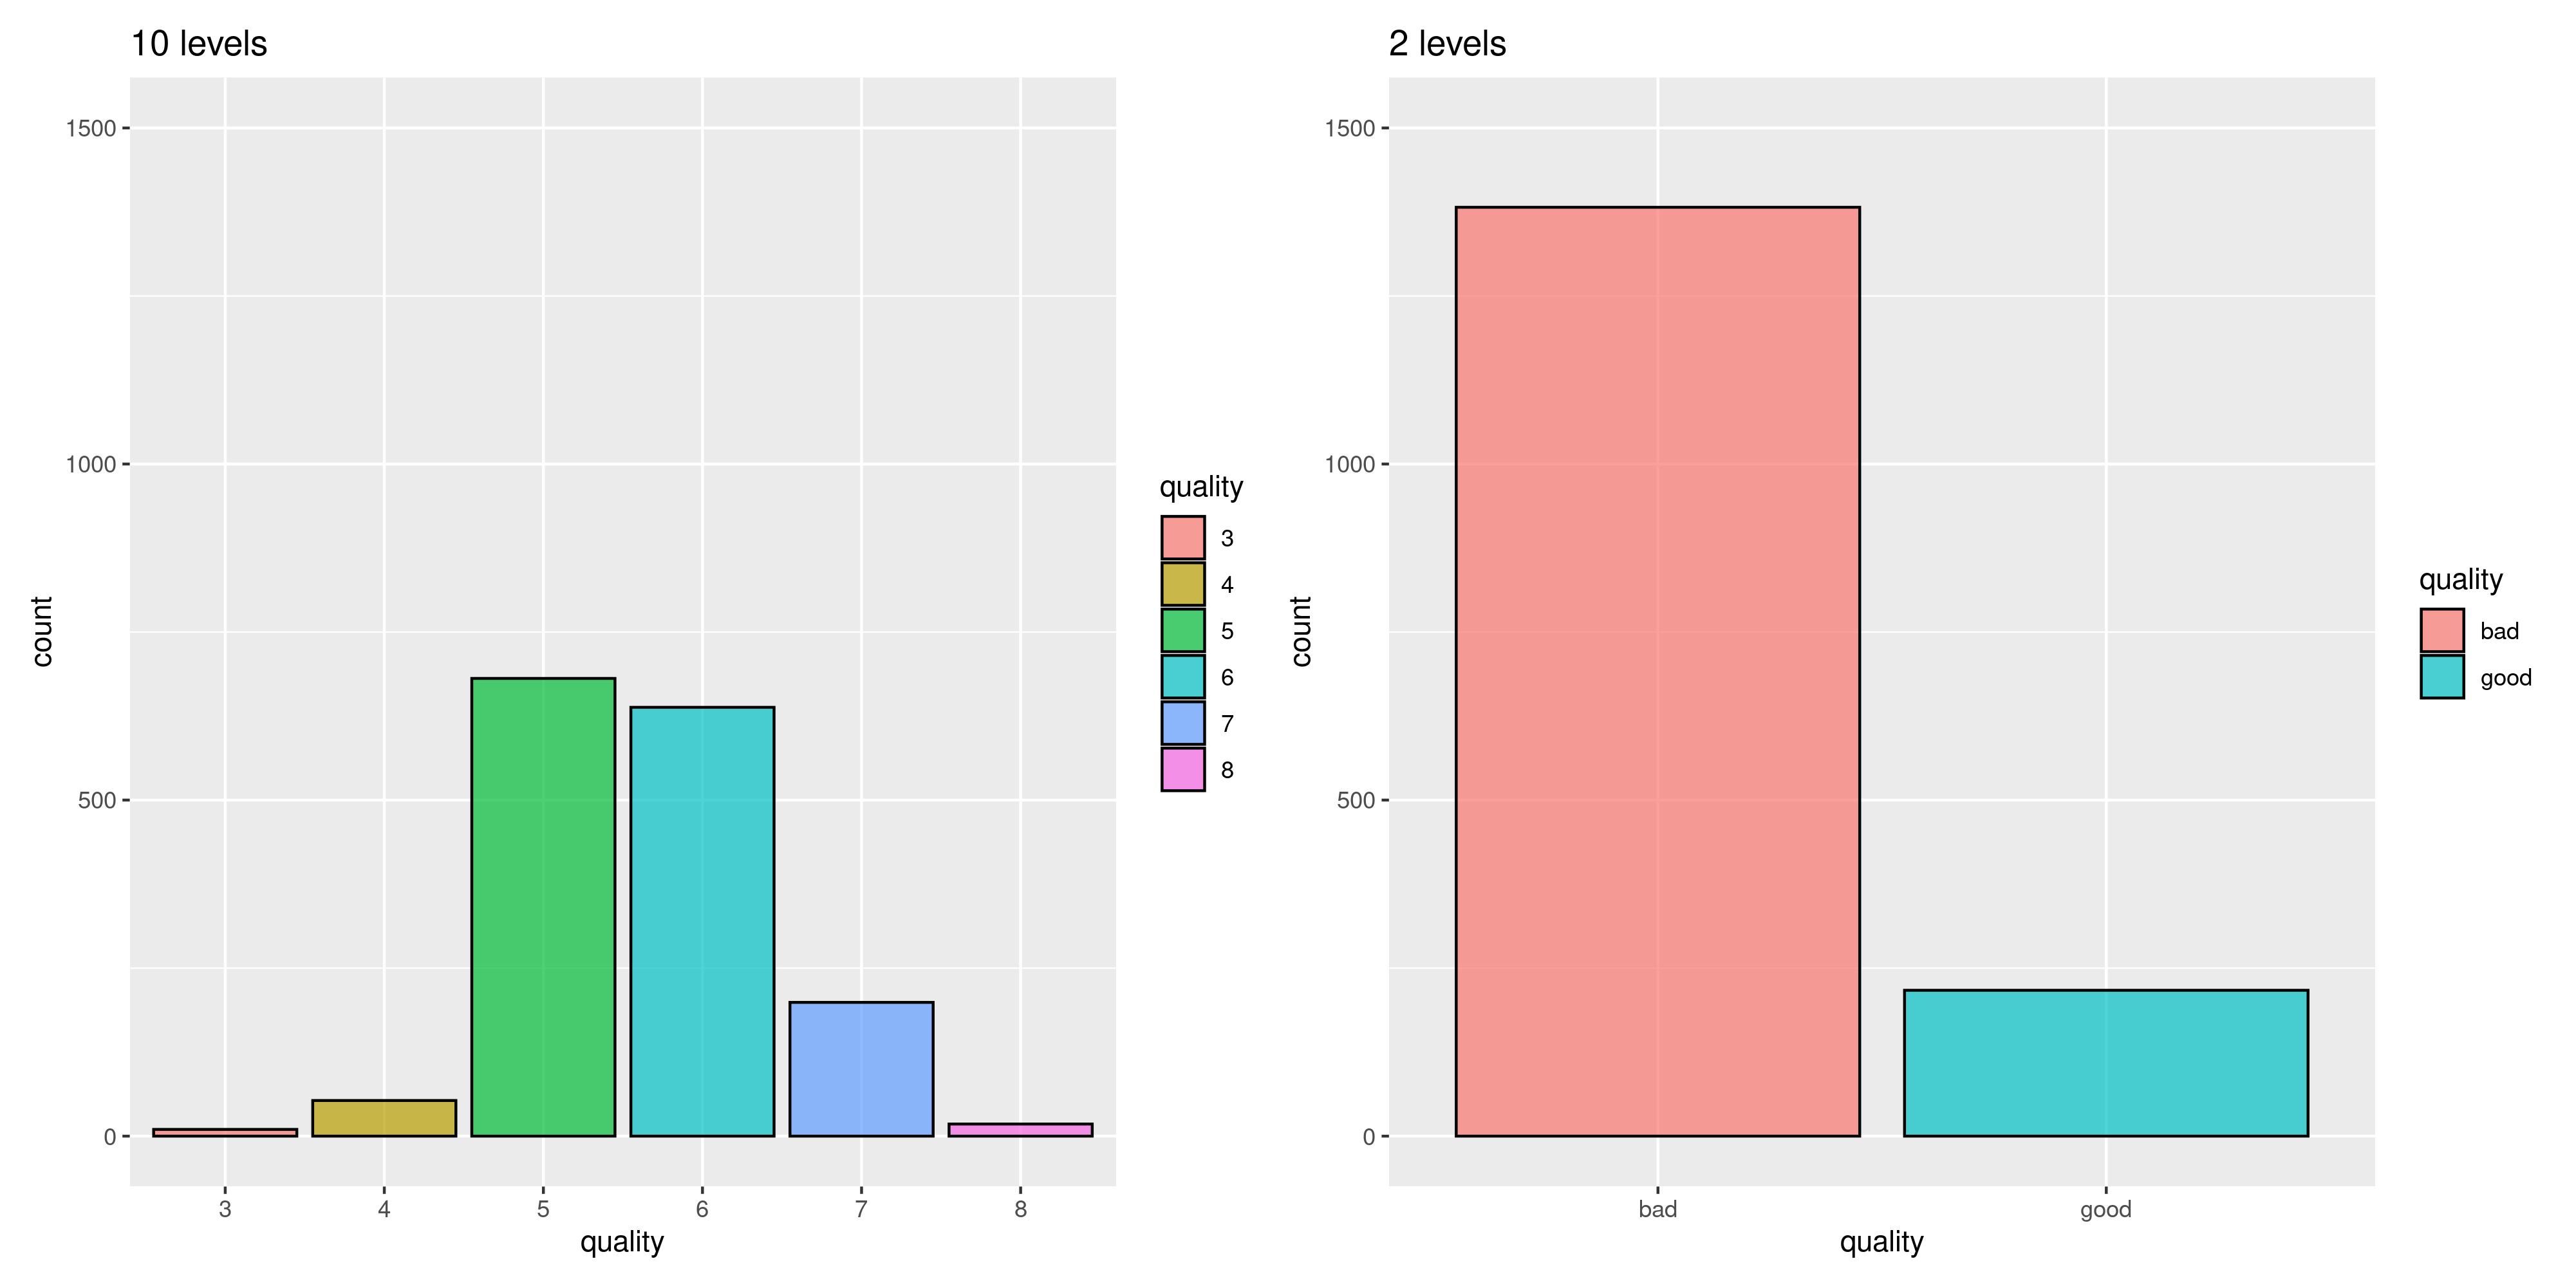
\includegraphics[width=\textwidth]{images/analisi/class_hist_binary.png}
    \caption{grafico che rappresenta la distribuzione dei dati rispetto alle due tipologie di classificazione prese in considerazione}
    \label{fig:quality_different_class}
\end{figure}

\noindent
Da questa analisi si è notato come le istanze non siano distribuite in modo uniforme, anzi si ha una prevalenza di dati rispetto alle qualità centrali e una scarsa rappresentazione delle qualità più basse e più alte, per questo motivo si è scartata l'ipotesi di poter sfruttare una classificazione a 10 classi, perché non in grado di rappresentare in modo appropriato le 10 classi.

\noindent
Osservando il grafico [\ref{fig:quality_different_class}] si può notare come per alcune classi di qualità non siano presenti istanze che li rappresentino.

\noindent
La classificazione a due classi è stata scelta perché anche se sbilanciata ha un buon numero di istanze che rappresentano sia la qualità bassa sia la qualità alta.

\noindent
Inoltre si è scelto di operare solamente usando una tipologia di vino perché operare considerando contemporaneamente vini bianchi e vini rossi rende più complessa la distinzione tra vini di bassa e alta qualità, questo per via delle loro diverse caratteristiche fisico-chimiche che li contraddistinguono.

\noindent
Quindi è stata considerata solamente la porzione di dataset relativa ai vini rossi, analogamente lo stesso procedimento può essere implementato per i vini bianchi. 
\chapter{Analisi Esplorativa}
\label{ch:analisi}

\chapter{Pre Processing}
\label{ch:preprocessing}
Il pre processing dei dati è una fase importate che consiste nel manipolare i dati attraverso varie trasformazioni e scelte.
Questa fase include la rimozione dei valori mancanti, un'eventuale scelta delle istanze da usare (campionamento, rimozione degli outliers), rimozione della ridondanza, trasformazioni sui dati come ad esempio normalizzazione, standardizzazione, \textit{feature extraction} e \textit{feature selection}.
Queste operazioni permettono di avere un input che passato ai modelli produce  risultati migliori.

\vspace{4mm}
\noindent
Il dataset originale è stato diviso in due sottoinsiemi, tenendo in ognuno di questi la stessa percentuale di istanze per classe (bad, good). Il training set contiene l'80\% del dataset, mentre il test set contiene il restante 20\%.

\vspace{4mm}
\noindent
Sul training set sono state applicate le seguenti strategie di pre processing:

\begin{itemize}
    \item Standardizzazione
    \item Standardizzazione + PCA
    \item Standardizzazione e rimozione outliers
    \item Standardizzazione + PCA e rimozione outliers
\end{itemize}

\newpage

\noindent
Per la standardizzazione vengono calcolate media $\mu$ e deviazione standard $\sigma$ per ogni variabile del training set, mentre per la PCA viene calcolata la matrice di rotazione $\text{W}$.
Queste misure vengono usate per effettuare il pre processing su entrambi i dataset $\text{X}$ (training e test).
La rimozione degli outliers viene effettuata attraverso il metodo scelto (IQR), prima di applicare le varie trasformazioni sui dati.

\vspace{4mm}
\begin{align*}
    \text{Z} &= \frac{\text{X} - \mu}{\sigma} \quad \text{(Standardizzazione)}
    \\\\
    \text{Z} &= \text{X} \text{W} \quad \text{(Trasformazione PCA)}
\end{align*}

\chapter{Modelli}
\label{ch:modelli}
In questo breve capitolo, oltre a presentare i modelli usati: CART e SVM, con le loro caratteristiche principali, verranno inoltre mostrati i rispettivi parametri di tuning scelti tramite grid search per i diversi tipi di pre processing sul dataset.

\section{CART (Classification And Regression Tree)}
CART è un algoritmo di classificazione supervisionato che costruisce un albero iterativamente. Ad ogni passo viene scelto l'attributo migliore secondo un criterio prestabilito e viene associato a un nodo.
L'arco verso un nodo figlio rappresenta un possibile valore per quell'attributo, mentre i nodi foglia rappresentano il valore predetto per il target.
E' stato scelto come criterio \textit{gini index}.

\begin{itemize}
    \item Sono poco soggetti agli outliers e ai valori mancanti
    \item Permettono di trovare una funzione non lineare 
    \item E' un algoritmo non parametrico, quindi non richiede assunzioni, tecniche di regolarizzazione apparte
    \item Molto soggetto a problematiche di overfitting se l'albero è profondo
    \item Sono poco costosi computazionalmente rispetto a SVM e Reti Neurali
    \item Non è necessario nessun pre processing al contrario delle SVM e delle Reti Neurali
\end{itemize}

\newpage

\subsection*{Tuning}Per CART la grid search prevede come un unico parametro ovvero la profondità massima dell'albero. Tramite la scelta di questo parametro è possibile ottenere un albero meno profondo e ridurre il rischio di overfitting.

\begin{itemize}
    \item \textbf{CART}: \textbf{max depth}: da 2 a 30
\end{itemize}

\begin{table}[H]
\centering
\begin{tabular}{|l|c|c|}
\hline
\textbf{pre processing} & \textbf{max depth} \\ \hline
Standardizzazione & 14 \\ \hline
Standardizzazione + PCA & 13 \\ \hline
Standardizzazione senza outliers & 9 \\ \hline
Standardizzazione + PCA senza outliers & 9 \\ \hline
\end{tabular}
\caption{Parametri migliori per CART per ogni pre processing}
\label{tab:my-table}
\end{table}

\section{SVM (Support Vector Machine)}
L'SVM è un algoritmo di classificazione supervisionato che ha come scopo trovare il miglior iperpiano che separa due classi, massimizzando il margine tra esse.

\begin{itemize}
    \item Nella versione soft margin permette una certa tolleranza agli outliers
    \item L'utilizzo dei metodi kernel consente di gestire la non linearità dei dati
    \item Richiede un pre processing dei dati al contrario di CART e Naive Bayes
    \item Al contrario di altri modelli come Naive Bayes e CART ha un grosso costo computazionale
    \item Rispetto alle Reti Neurali richiede meno dati per essere trainato
\end{itemize}

\newpage

\subsection*{Tuning}
Per l'SVM sono stati usati diversi kernel: lineare, polinomiale e radiale. Per ognuno di essi vengono riportati i parametri su i quali viene effettuata la grid search.

\begin{table}[H]
\centering
\resizebox{\textwidth}{!}{%
\begin{tabular}{|c|c|c|c|c|}
\hline
\textbf{models} & \textbf{C} & \textbf{sigma} & \textbf{degree} & \textbf{scale} \\ \hline
lineare & range & \textbackslash{} & \textbackslash{} & \textbackslash{} \\ \hline
polinomiale & range & \textbackslash{} & 2,3,4,5,6 & 1/numero di features \\ \hline
radiale & range & range & \textbackslash{} & \textbackslash{} \\ \hline
\end{tabular}%
}
\caption{Parametri utilizzati per la grid search per i vari metodi kernel, range = (0.01, da 0.1 a 1.5 con passo 0.1, 2, 5, 10)}
\label{tab:my-table}
\end{table}

\begin{table}[H]
\centering
\begin{tabular}{|l|c|c|}
\hline
\textbf{pre processing} & \textbf{C} \\ \hline
Standardizzazione & 1.1 \\ \hline
Standardizzazione + PCA & 0.4 \\ \hline
Standardizzazione senza outliers & 1 \\ \hline
Standardizzazione + PCA senza outliers & 1.2 \\ \hline
\end{tabular}
\caption{Parametri migliori per la SVM con kernel lineare per ogni pre processing}
\label{tab:my-table}
\end{table}

\begin{table}[H]
\centering
\begin{tabular}{|l|c|c|c|}
\hline
\textbf{pre processing} & \textbf{C} & \textbf{sigma} \\ \hline
Standardizzazione & 0.01 & 2 \\ \hline
Standardizzazione + PCA & 0.01 & 2 \\ \hline
Standardizzazione senza outliers & 2 & 1.4 \\ \hline
Standardizzazione + PCA senza outliers & 0.4 & 1.4 \\ \hline
\end{tabular}
\caption{Parametri migliori per la SVM con kernel radiale per ogni pre processing}
\label{tab:my-table}
\end{table}

\begin{table}[H]
\centering
\begin{tabular}{|l|c|c|c|c|}
\hline
\textbf{pre processing} & \textbf{C} & \textbf{scale} & \textbf{degree}\\ \hline
Standardizzazione & 0.4 & 0.09090 & 2 \\ \hline
Standardizzazione + PCA & 0.01 & 0.11111 & 2 \\ \hline
Standardizzazione senza outliers & 0.01 & 0.09090 & 2 \\ \hline
Standardizzazione + PCA senza outliers & 0.1 & 0.11111 & 2 \\ \hline
\end{tabular}
\caption{Parametri migliori per la SVM con kernel polinomiale per ogni pre processing}
\label{tab:my-table}
\end{table}

\chapter{Esperimenti}
In questo capitolo vengono mostrati i vari esperimenti fatti in base al pre processing utilizzato. 
I vari modelli vengono addestrati utilizzando una k-fold cross validation.
La cross validation necessità di essere eseguita in modo appropriato poiché il dataset in esame è sbilanciato.
Vista la numerosità della classe minoritaria si è fissato k=5 rispetto al solito valore di k=10 in modo da avere dei sottoinsiemi significativi.
Inoltre la cross validation viene effettuata in modo stratificato, così da avere in ogni fold in proporzione lo stesso numero di istanze positive e negative, poiché altrimenti potrebbe accadere che un fold abbia pochi elementi della classe minoritaria.
La cross validation viene effettuata 5 volte e alla fine viene scelto il modello che massimizza l'AUC (Area Under The Curve) della PRC (Precision Recall Curve). Questa metrica è comunemente utilizzata in caso di dati sbilanciati, l'accuracy in questi casi potrebbe portare a risultati errati, poiché si concentra prevalentemente sulla classe maggioritaria.
I vari esperimenti verranno mostrati di seguito nel seguente ordine, prima verranno confrontate i vari metodi kernel per l'SVM, dopodiché l'SVM migliore verrà confrontata con CART, infine, dopo aver scelto il pre processing migliore, verranno confrontati i due modelli migliori.

\newpage

\section{Confronto tra i kernel per SVM}
I seguenti istogrammi comparano le performance ottenute tramite i diversi kernel utilizzati per i diversi tipi di pre processing utilizzati.
Le metriche adottate sono Accuracy, AUC PRC, F1, Precision, Recall.
Da essi è possibile notare come con il kernel radiale si assumono valori più alti del kernel polinomiale in presenza di outliers.
Rimuovendo gli outliers invece, il kernel polinomiale supera il kernel radiale in F1 e Recall. 
Dai risultati dell'SVM lineare si può pensare che i dati non siano linearmente separabili.

\begin{figure}[H]
    \centering

    \subfloat[Standardizzazione]{%
        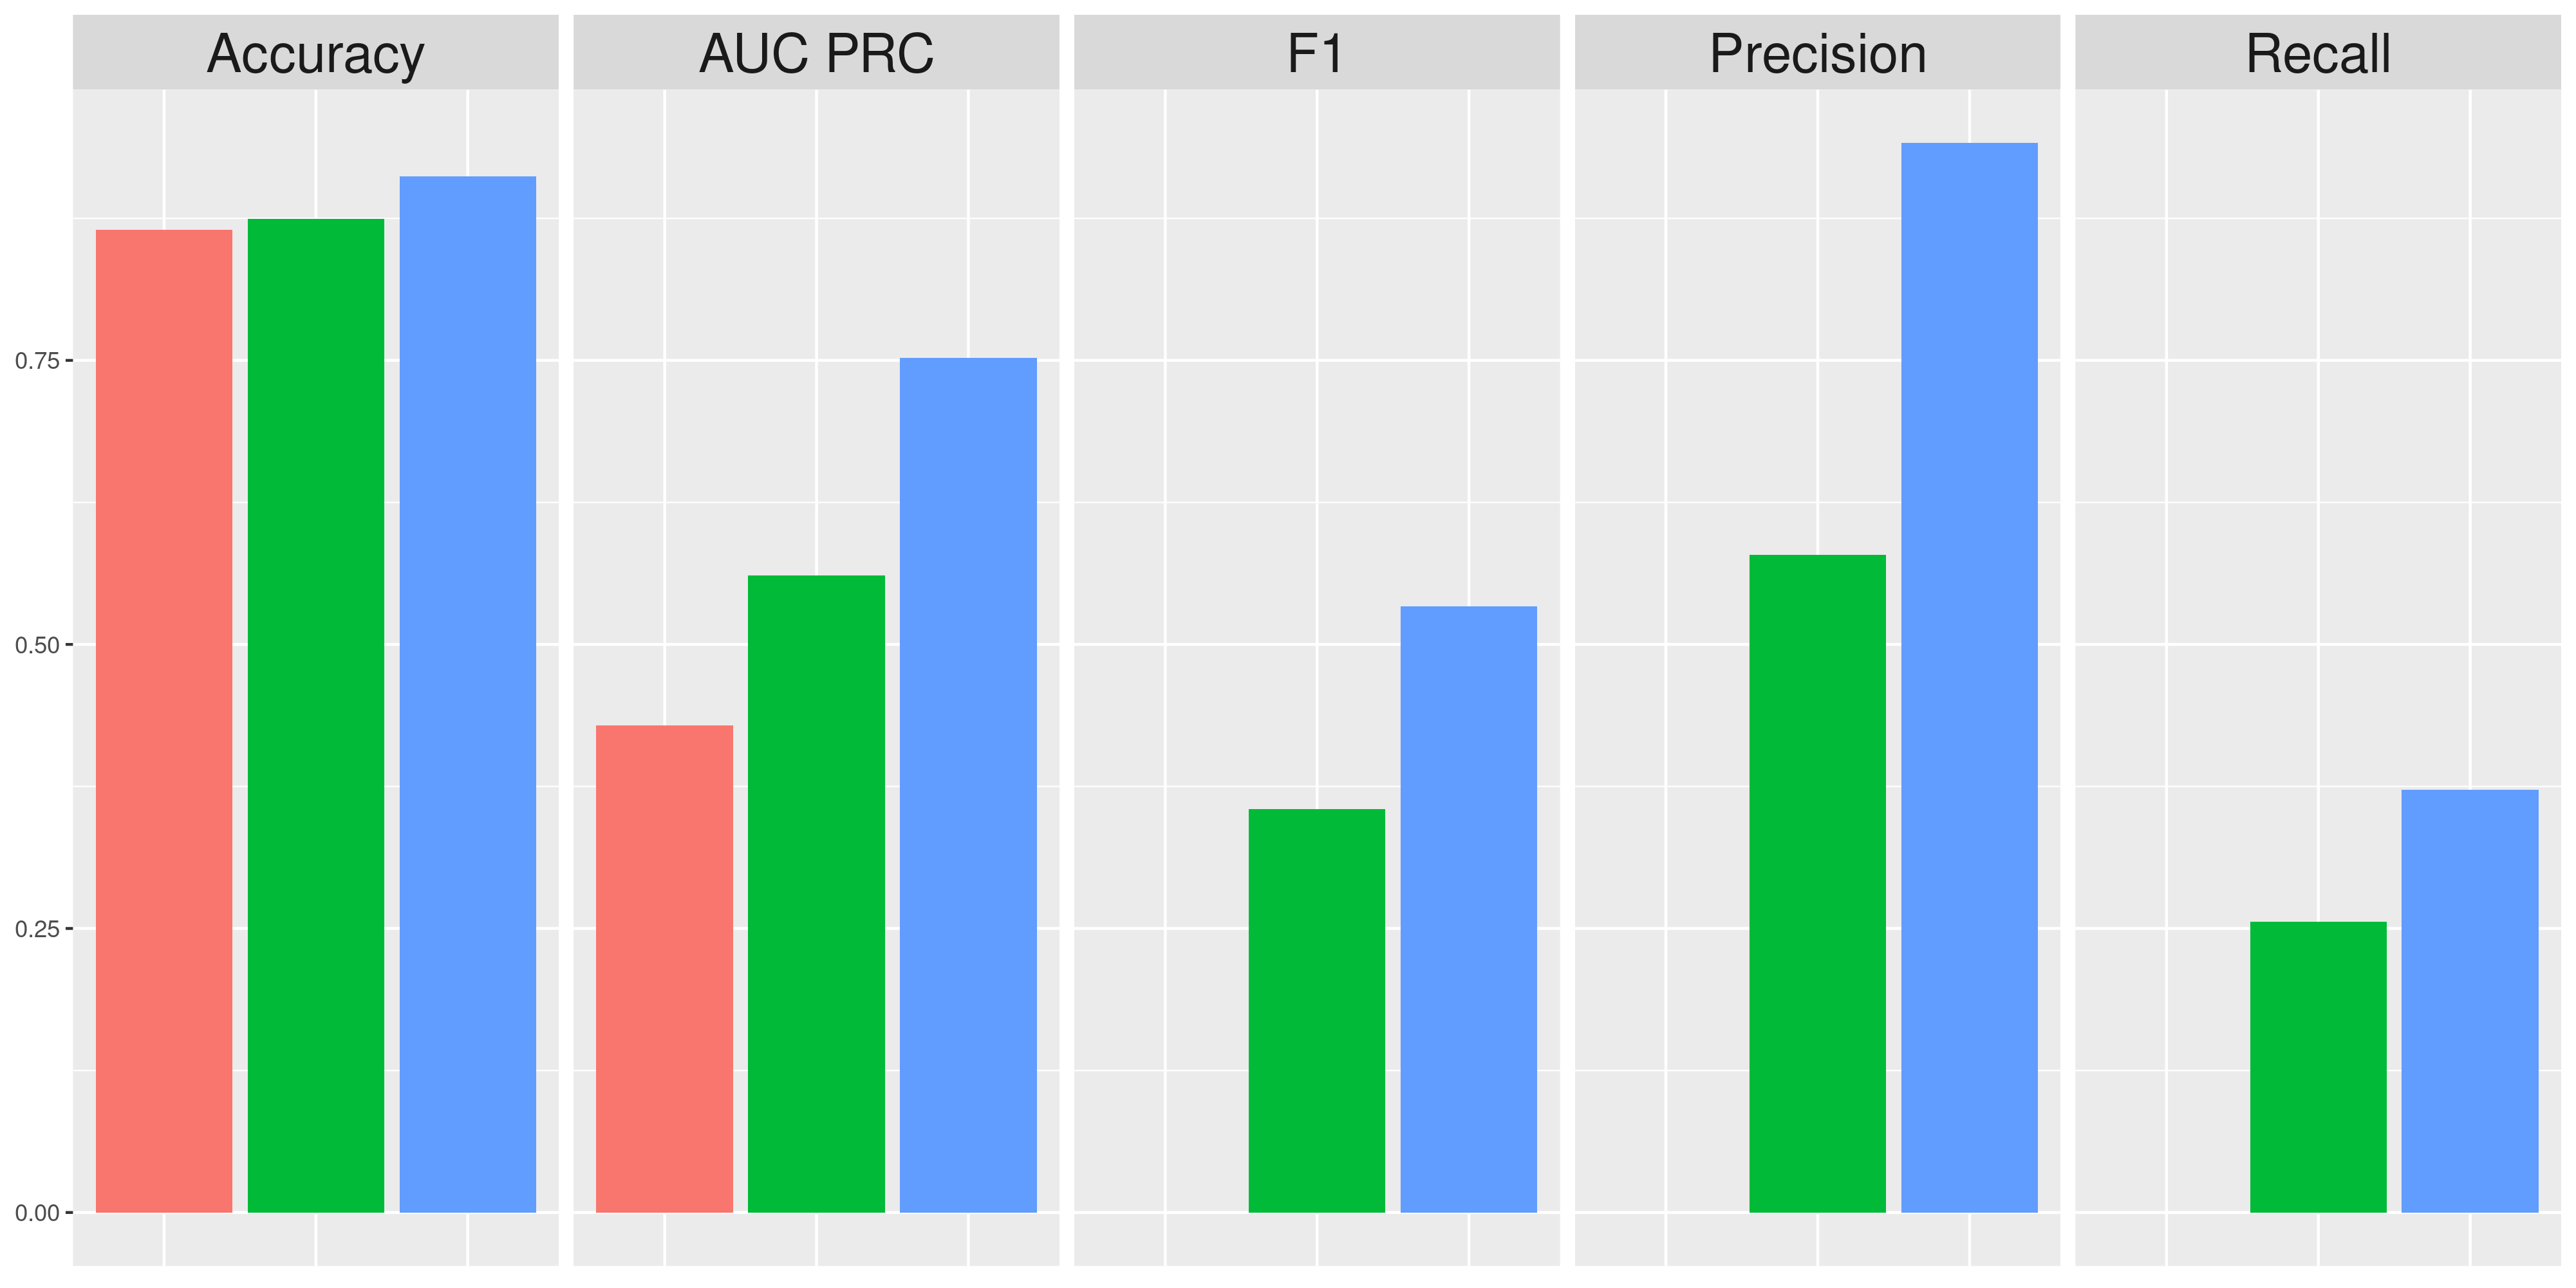
\includegraphics[width=12cm, height=8cm, keepaspectratio]{images/comparison/outliers/kernel/z-score_measures.png}
    }
    \quad
    \subfloat[Standardizzazione + PCA]{%
        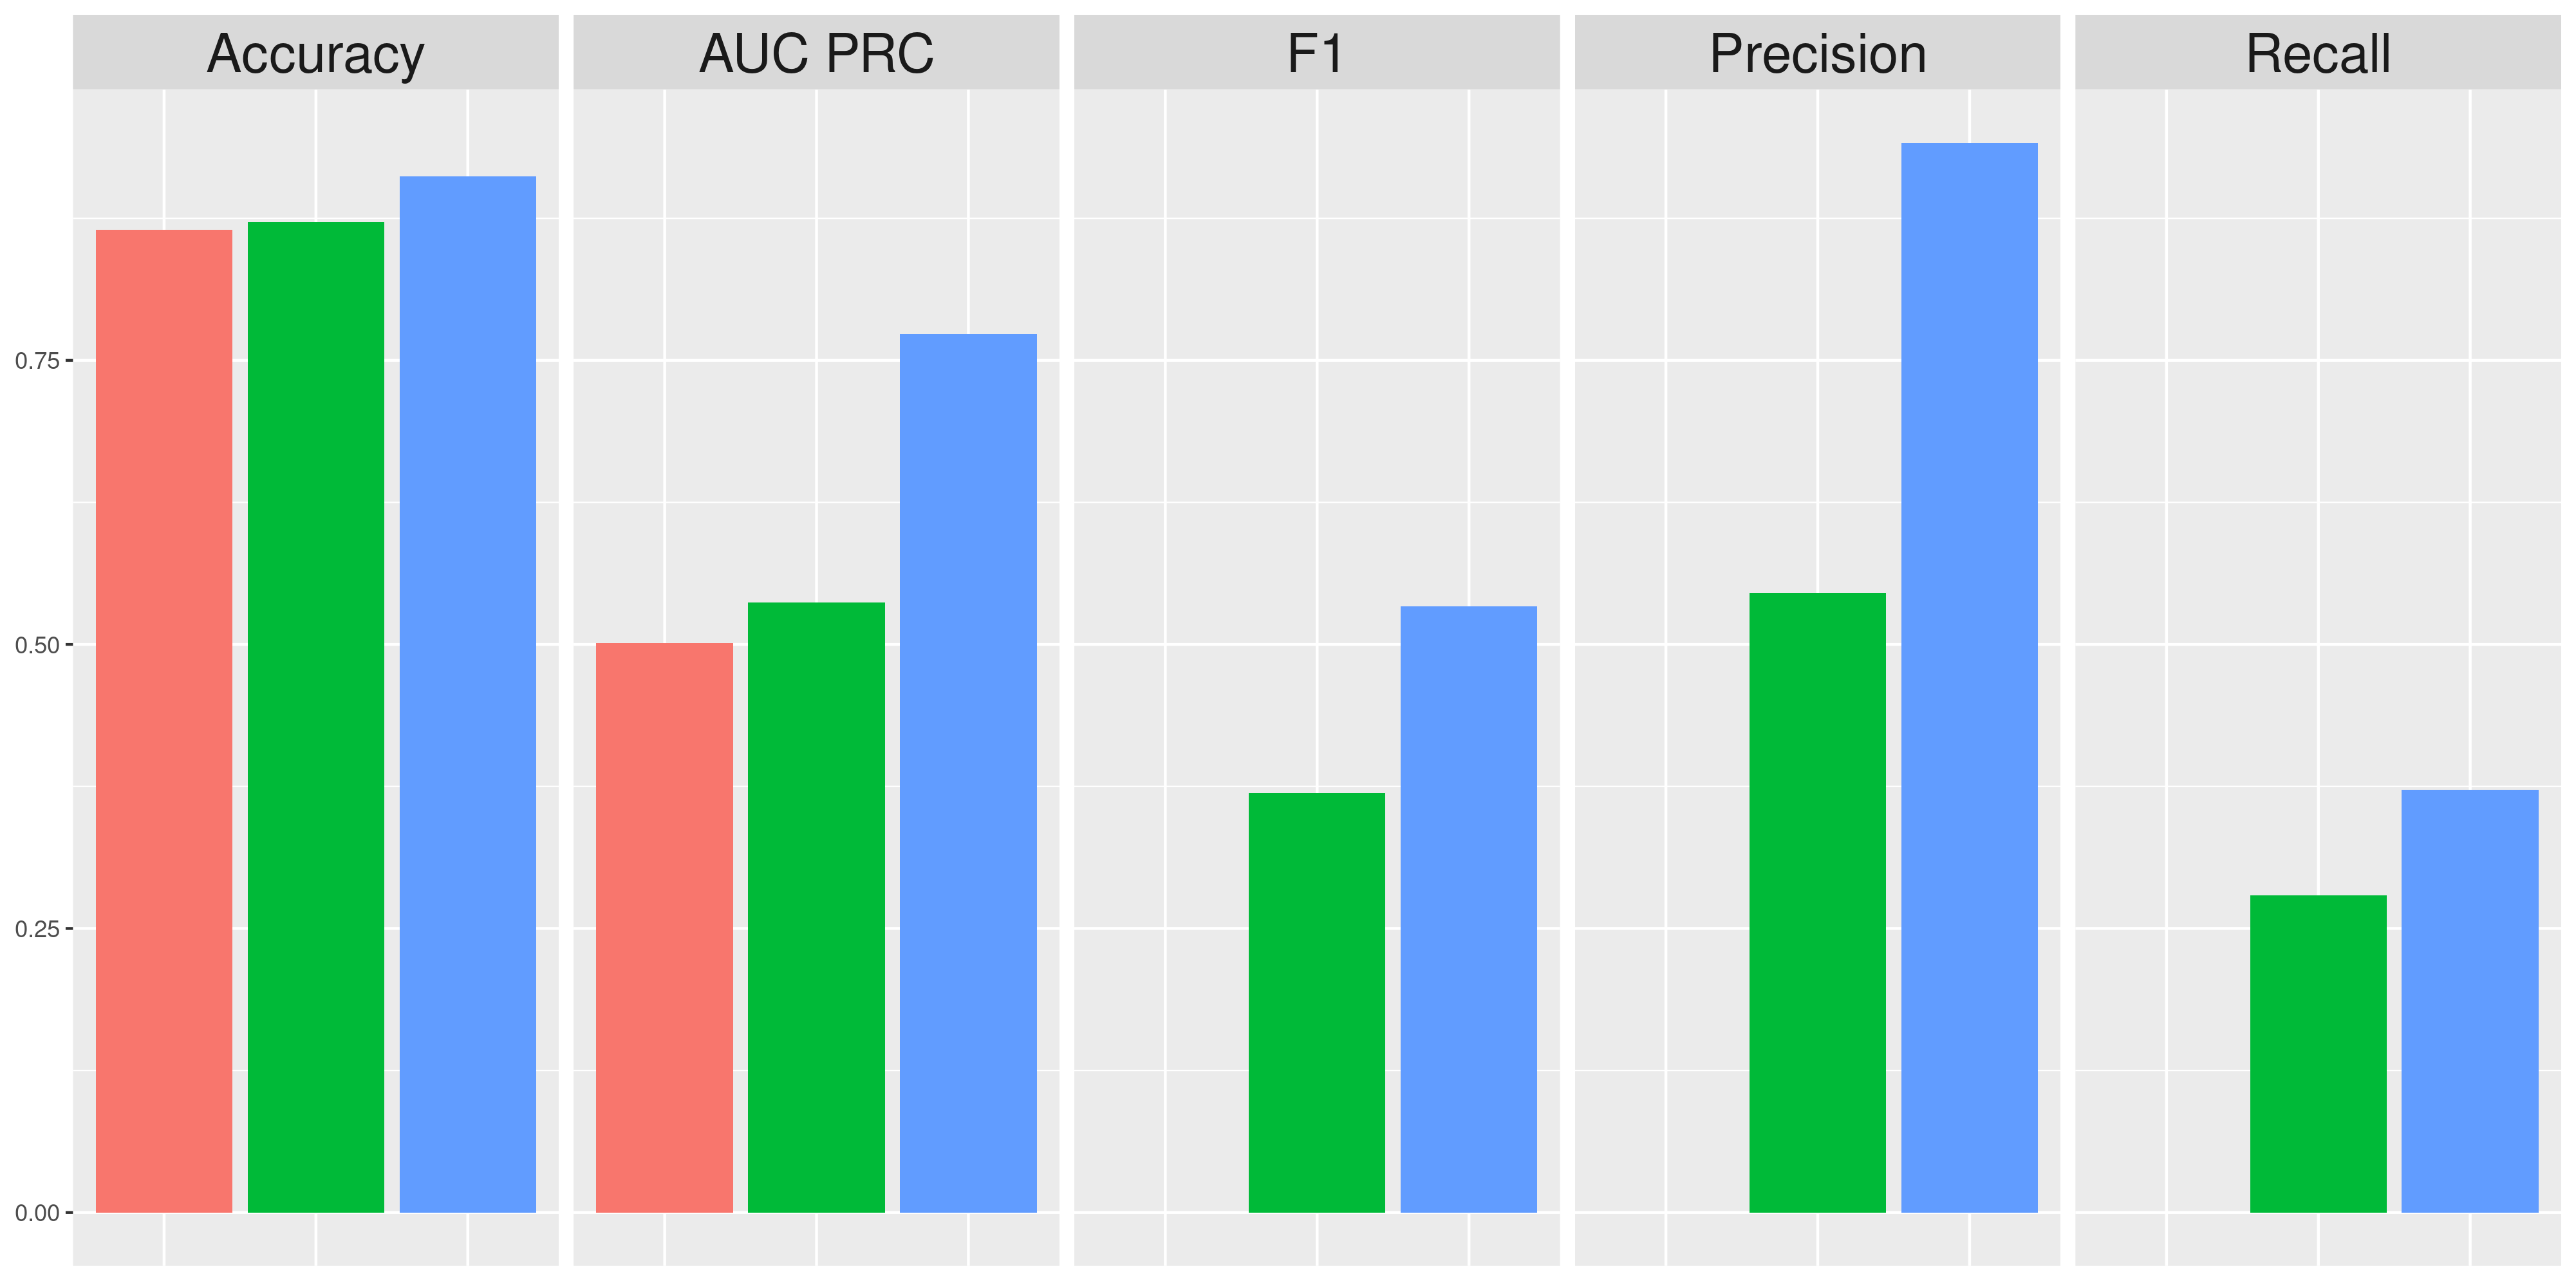
\includegraphics[width=12cm, height=8cm, keepaspectratio]{images/comparison/outliers/kernel/pca_measures.png}
    }

    \label{fig:measures_svm_outliers}
    \caption{Risultati della SVM con i diversi kernel (lineare: rosso, polinomiale: verde, radiale: blu) sul testset con outliers}
\end{figure}

\begin{figure}[H]
    \centering

    \subfloat[Standardizzazione]{%
        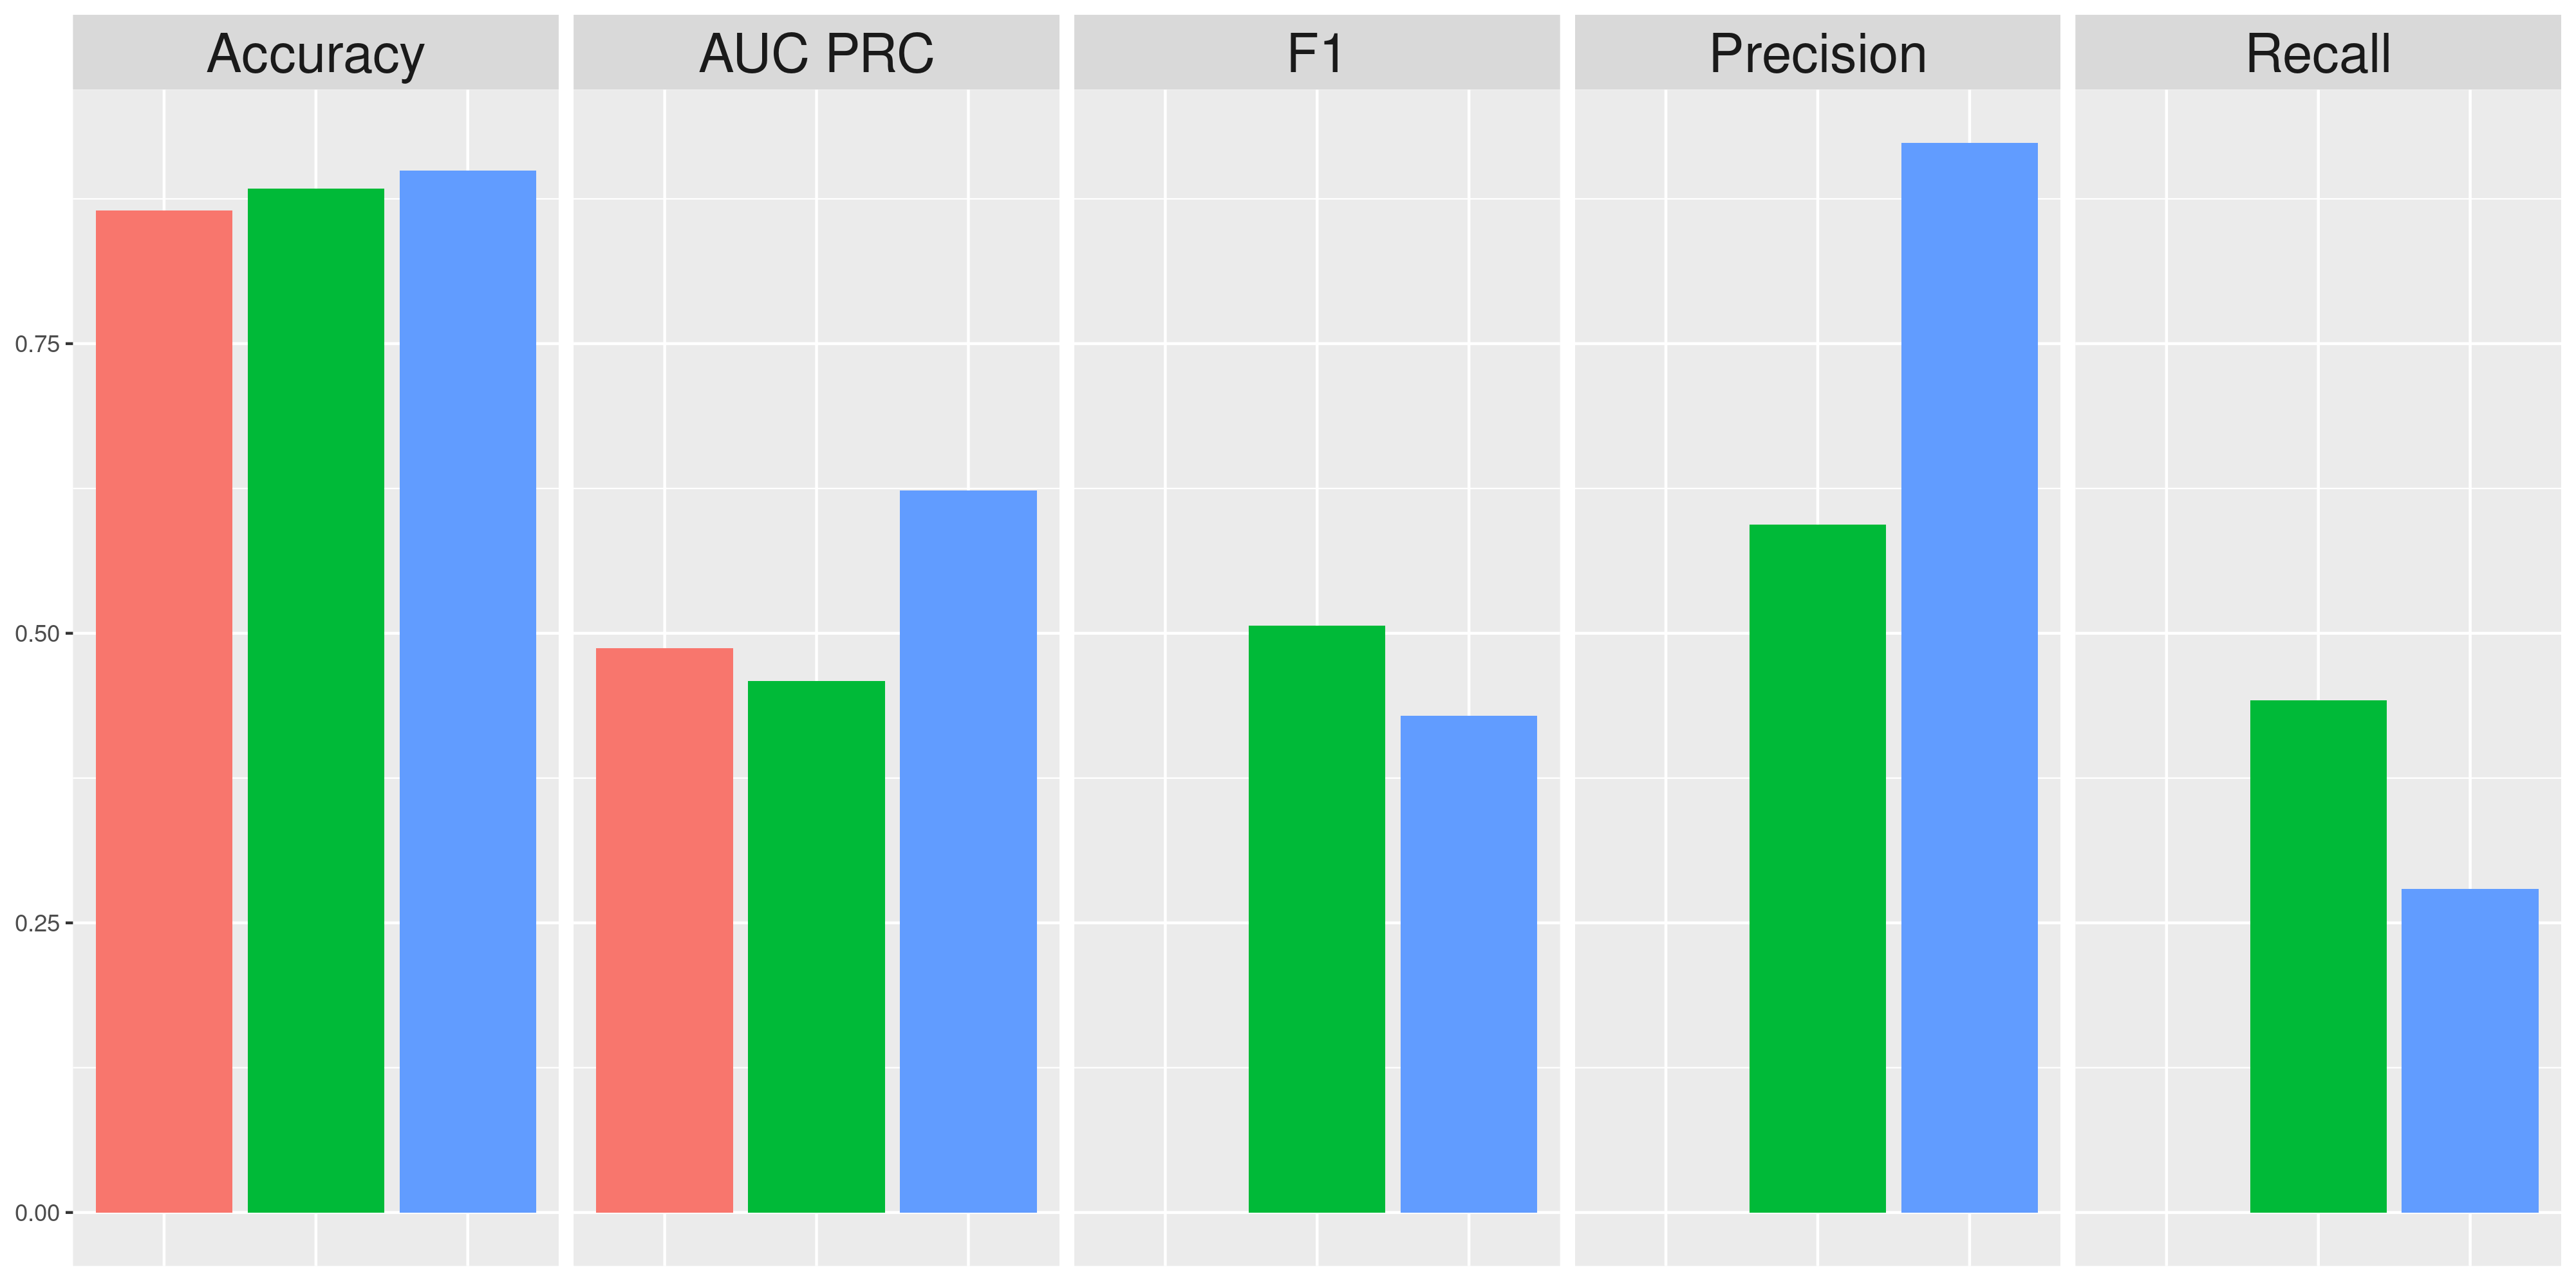
\includegraphics[width=12cm, height=8cm, keepaspectratio]{images/comparison/no-outliers/kernel/z-score_measures.png}
    }
    \quad
    \subfloat[Standardizzazione + PCA]{%
        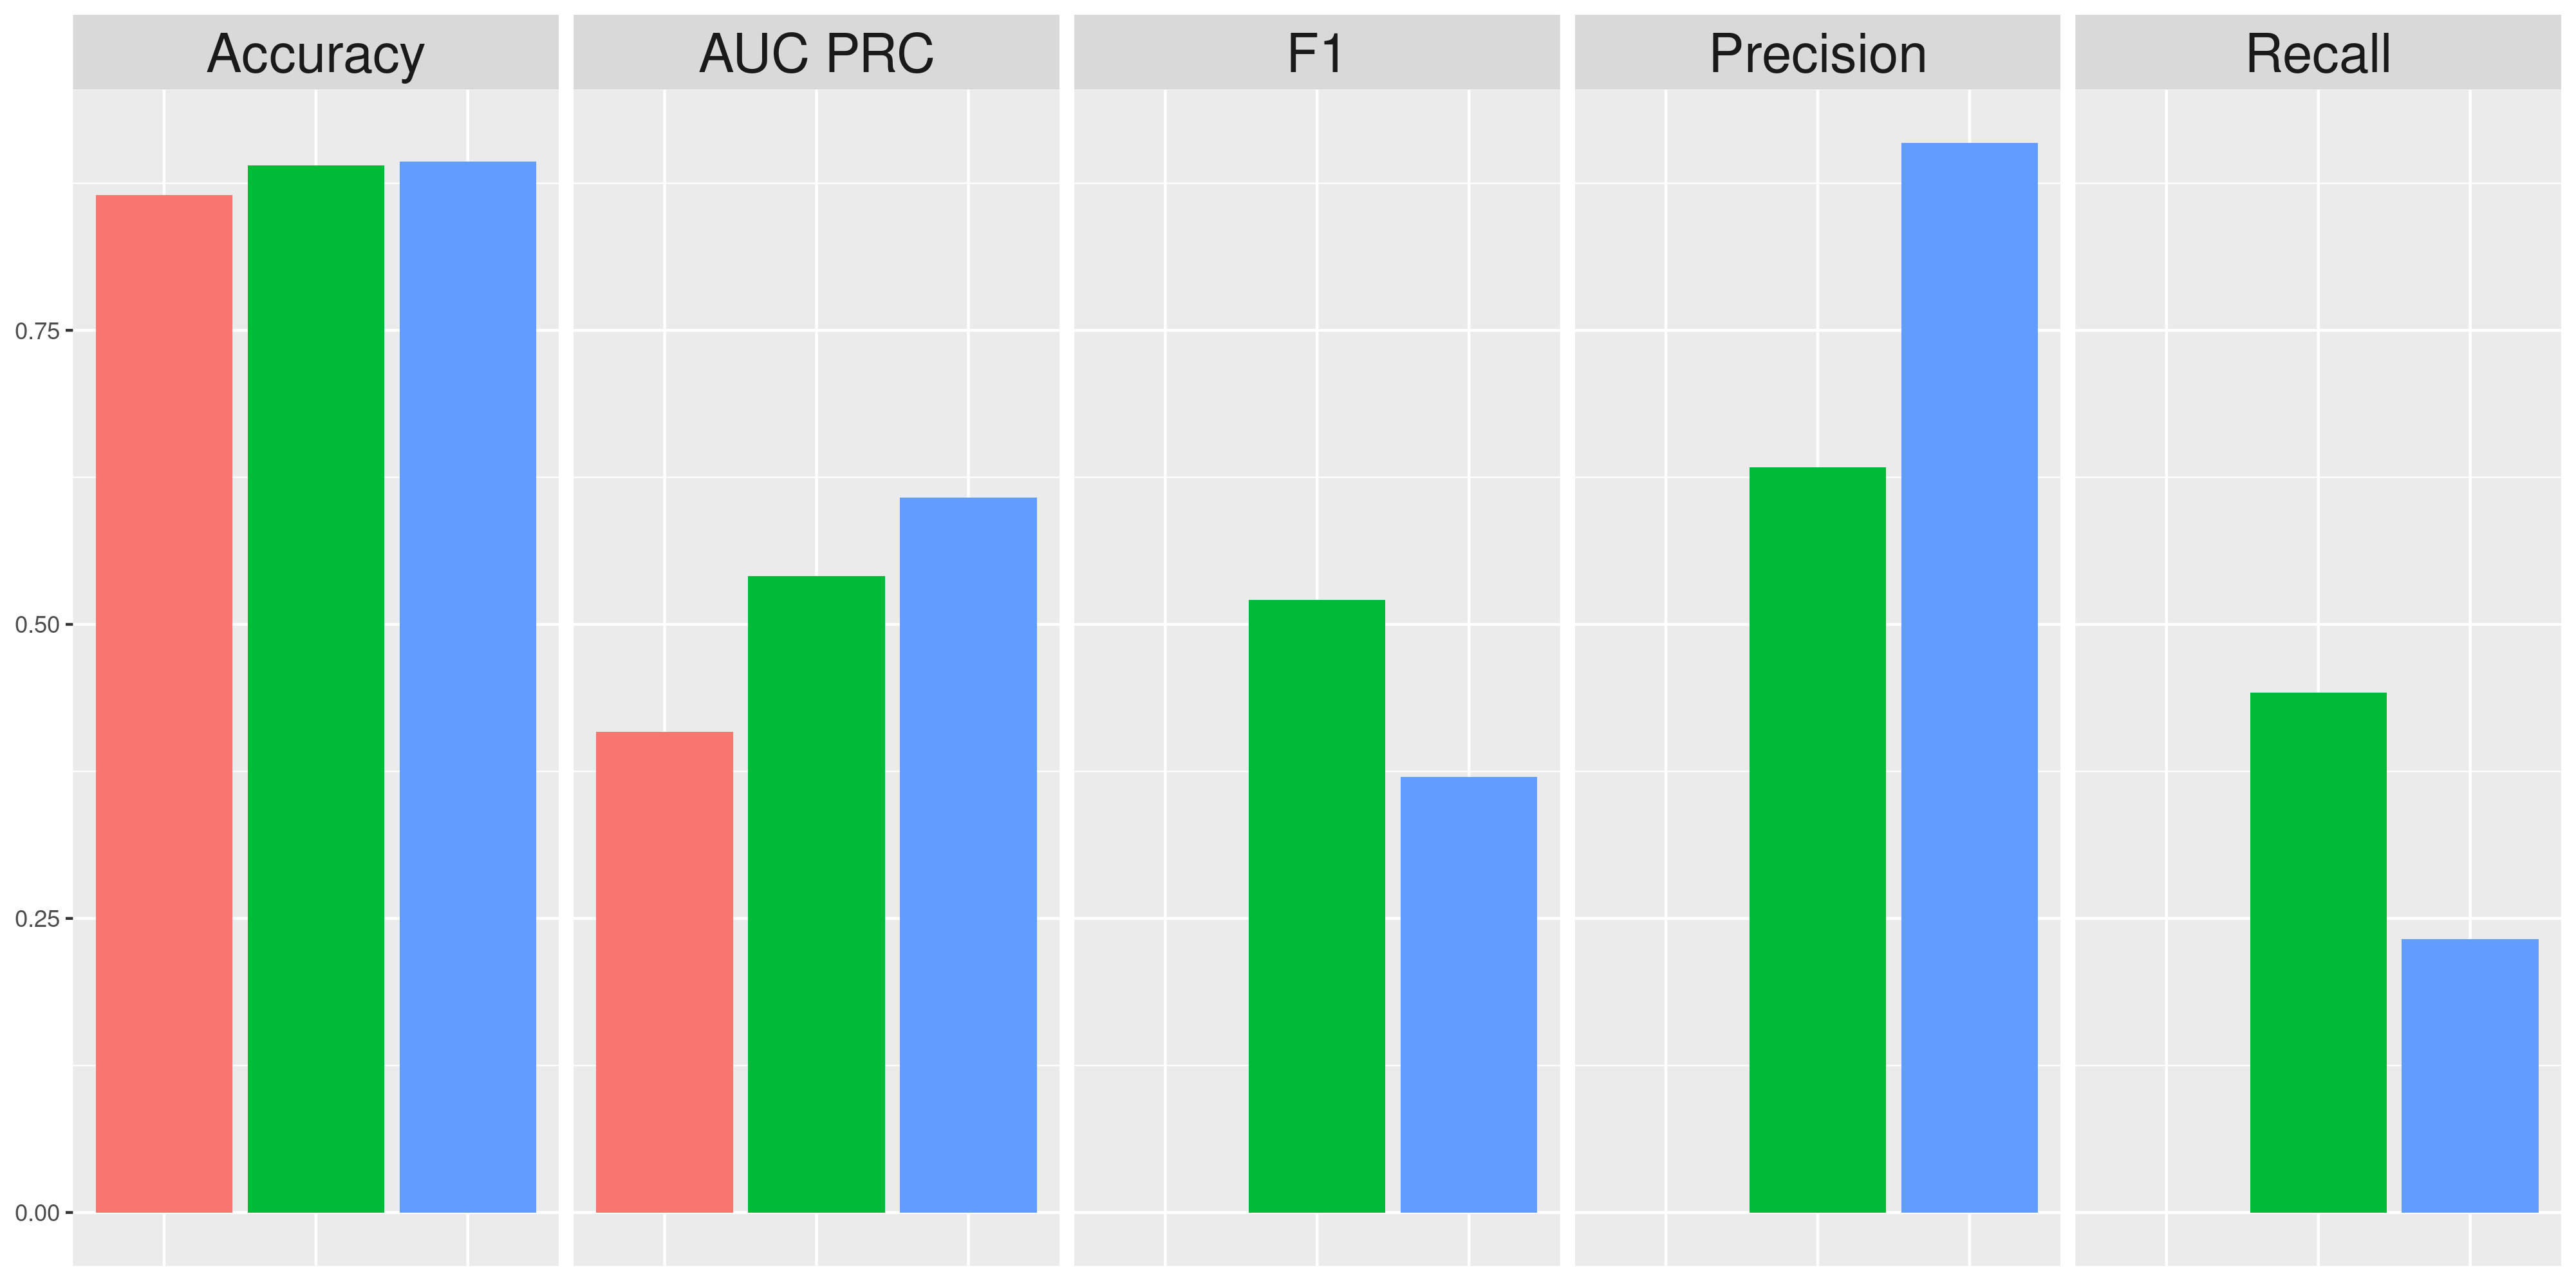
\includegraphics[width=12cm, height=8cm, keepaspectratio]{images/comparison/no-outliers/kernel/pca_measures.png}
    }

    \label{fig:measures_svm}
    \caption{Risultati della SVM con i diversi kernel (lineare: rosso, polinomiale: verde, radiale: blu) sul testset senza outliers}
\end{figure}

\noindent
Mostriamo ora graficamente la curva ROC (Receiver Operating Characteristic) e la PRC (Precision Recall Curve) che è più sensibile a situazioni con dati sbilanciati.
Infatti si può notare come le differenze tra i vari modelli siano molto grandi rispetto alla PRC, invece rispetto alla ROC tutti i modelli sono molto simili.
Inoltre la rimozione degli outliers comporta una perdita drastica nelle performance dei modelli.

\newpage

\begin{figure}[H]
    \centering

    \subfloat[Standardizzazione]{%
        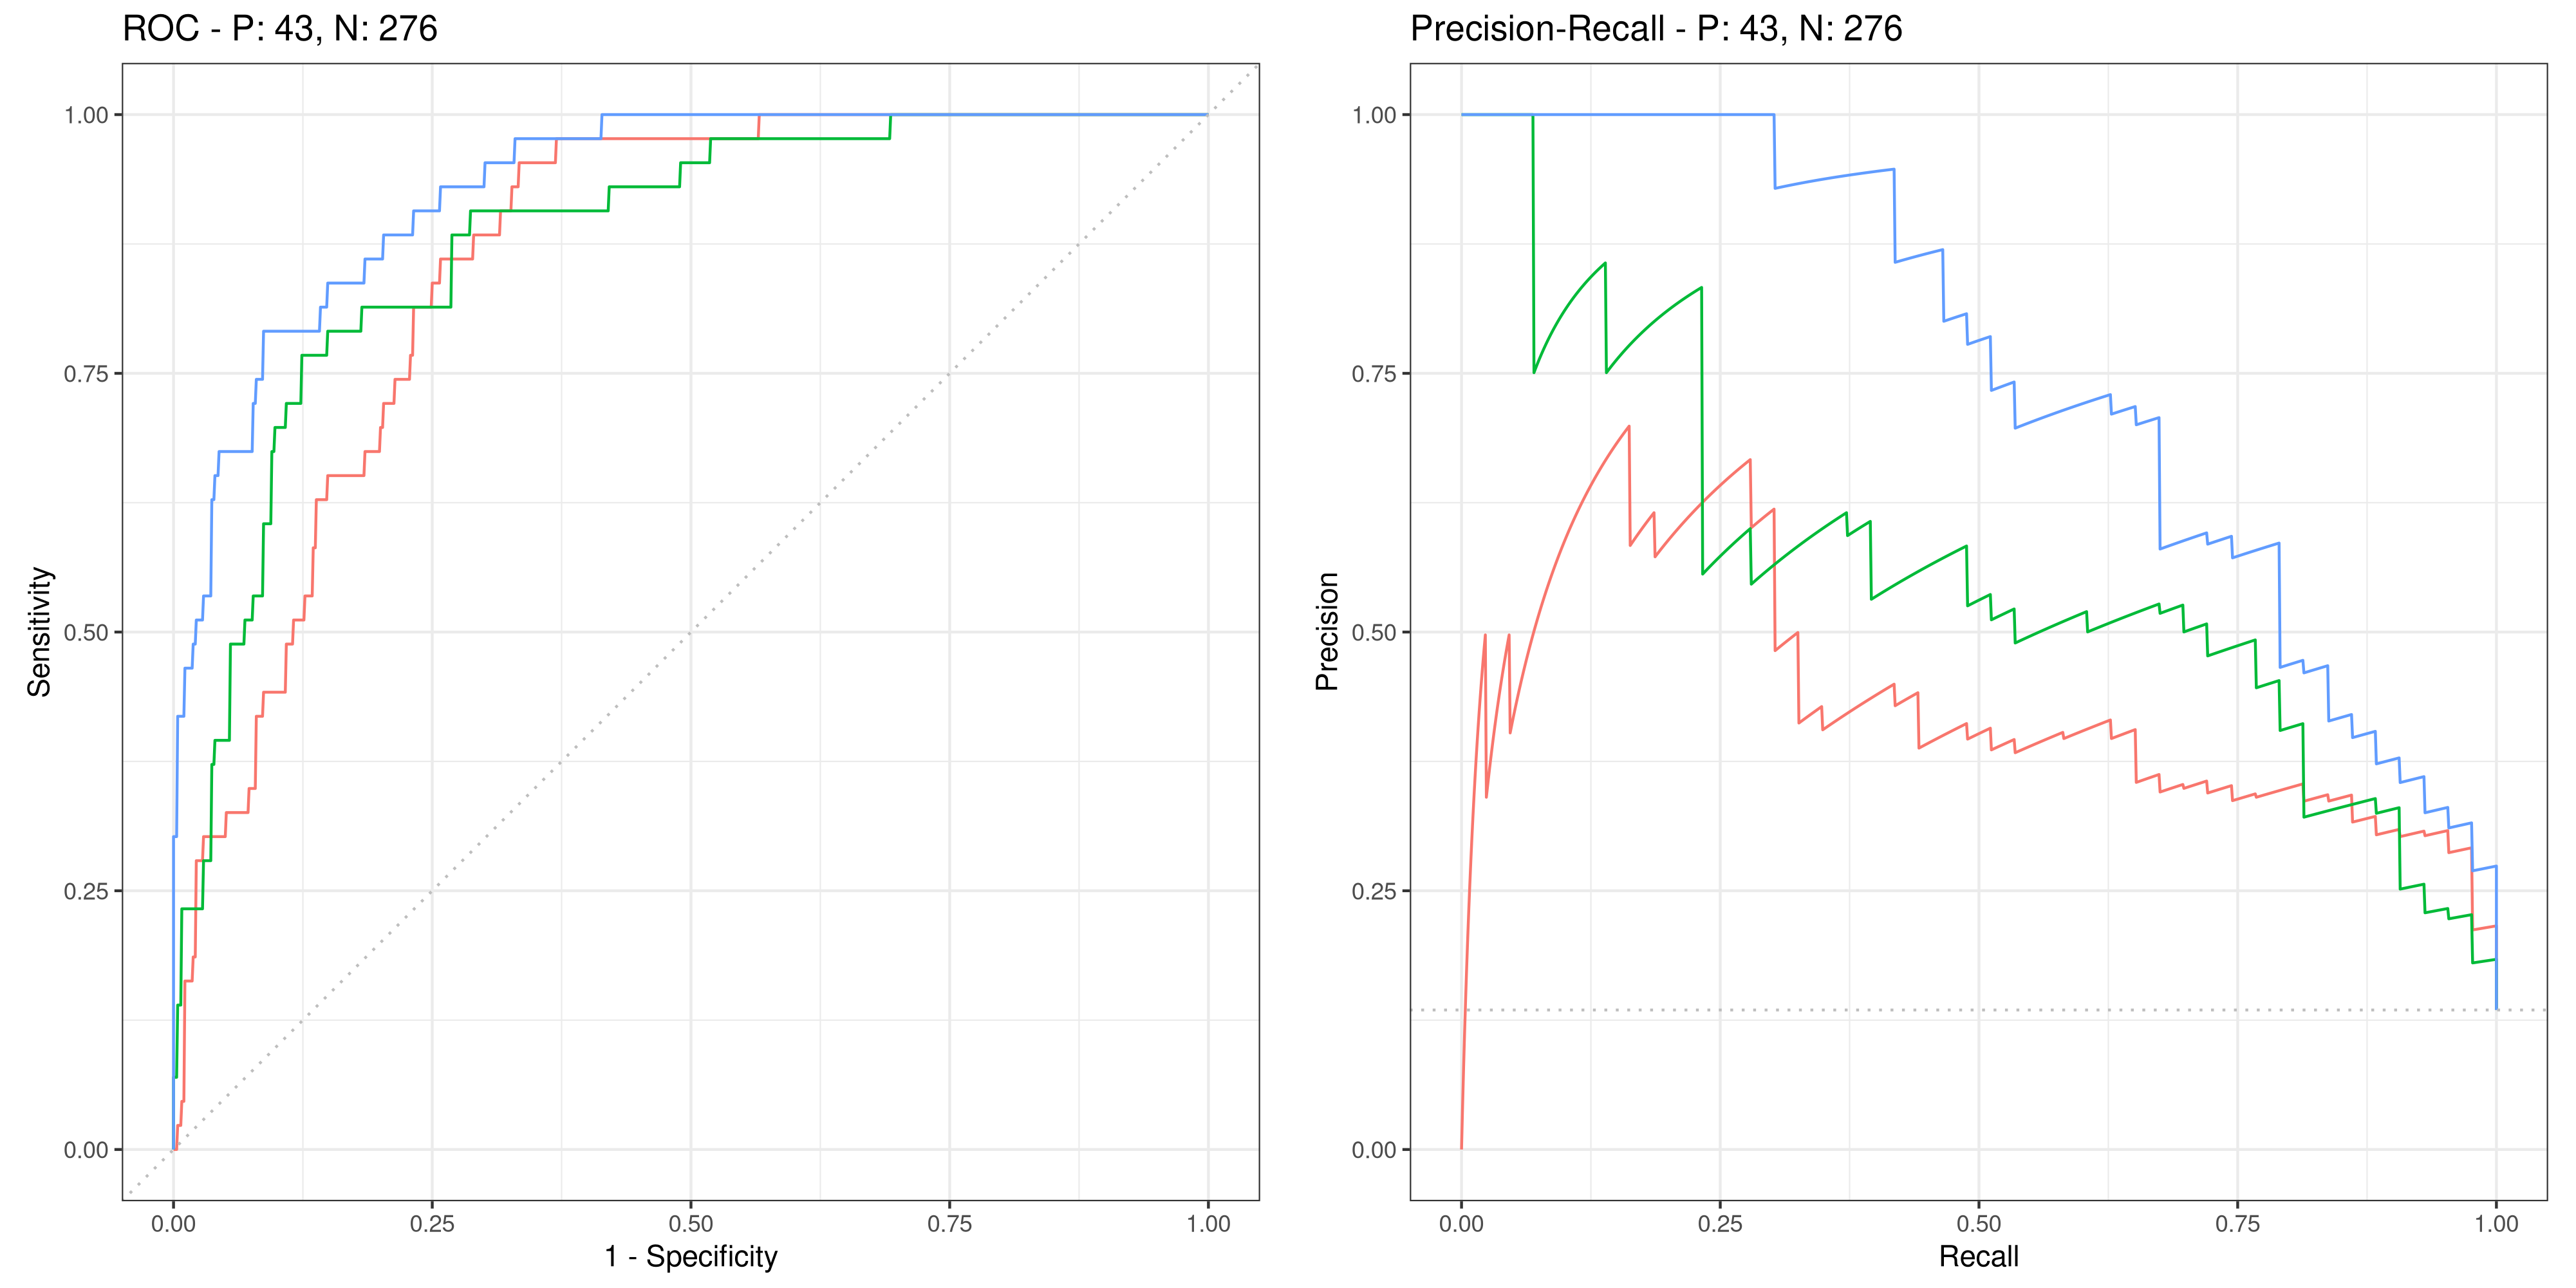
\includegraphics[width=\linewidth]{images/roc/outliers/kernel/z-score.png}
    }
    \quad
    \subfloat[Standardizzazione + PCA]{%
        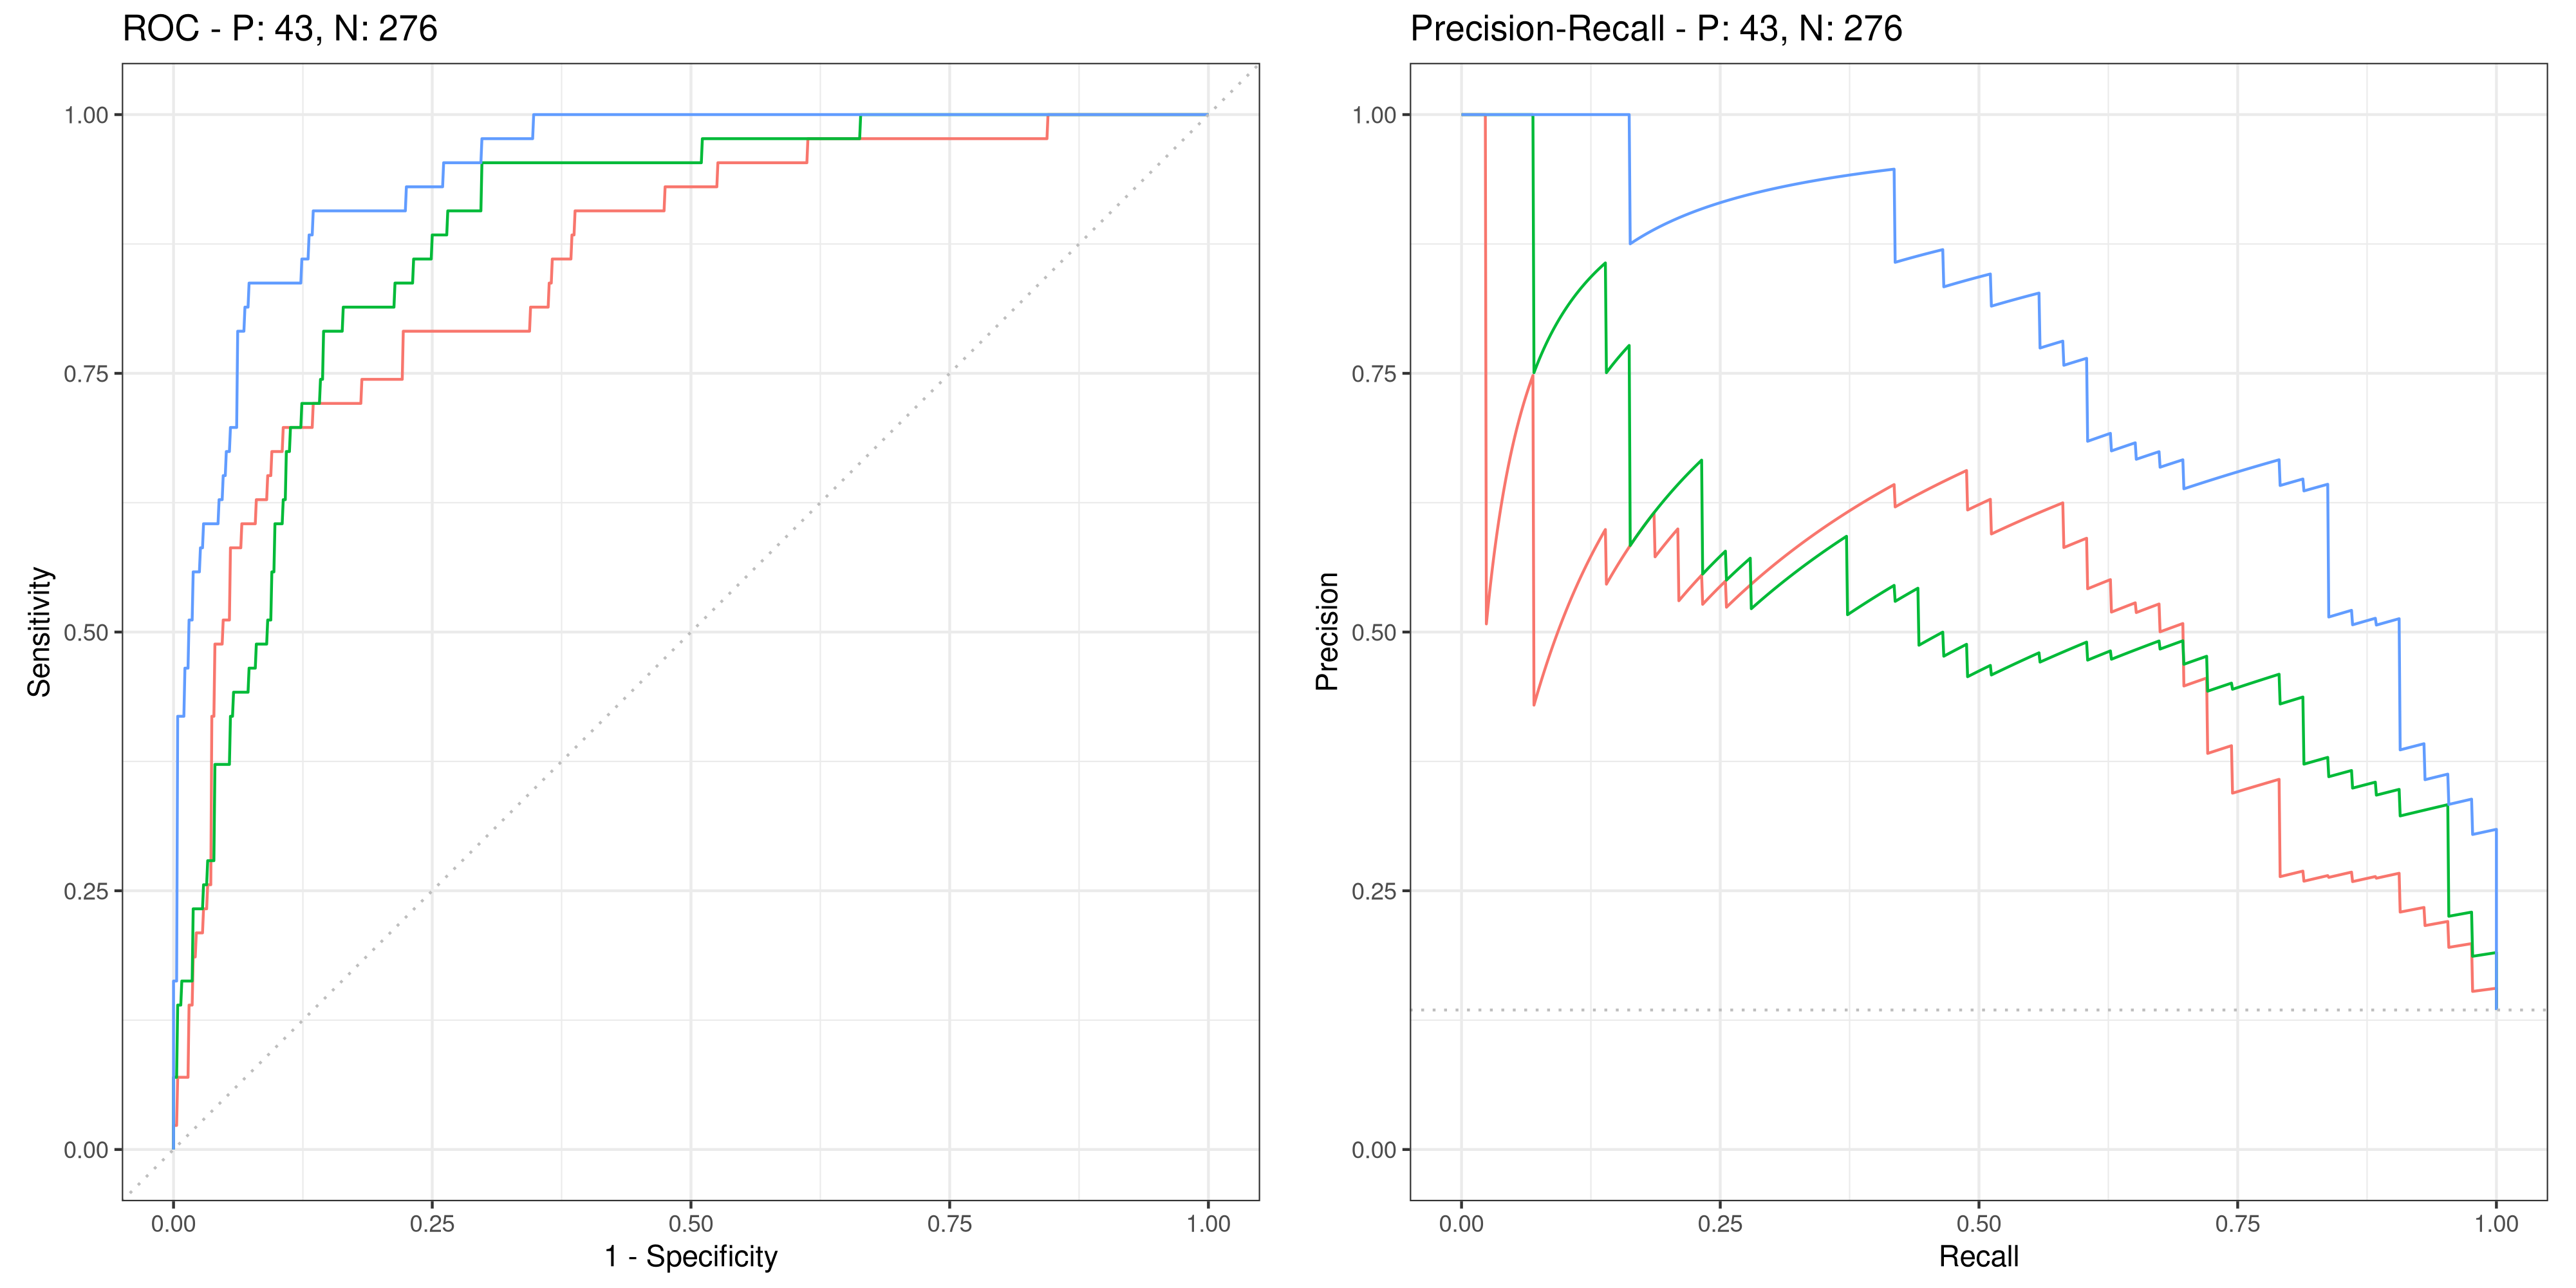
\includegraphics[width=\linewidth]{images/roc/outliers/kernel/pca.png}
    }
    \label{fig:roc_svm_outliers}
    \caption{Curve ROC e PRC per i diversi kernel (lineare: rosso, polinomiale: verde, radiale: blu) sul testset con outliers}
\end{figure}

\begin{figure}[H]
    \centering

    \subfloat[Standardizzazione]{%
        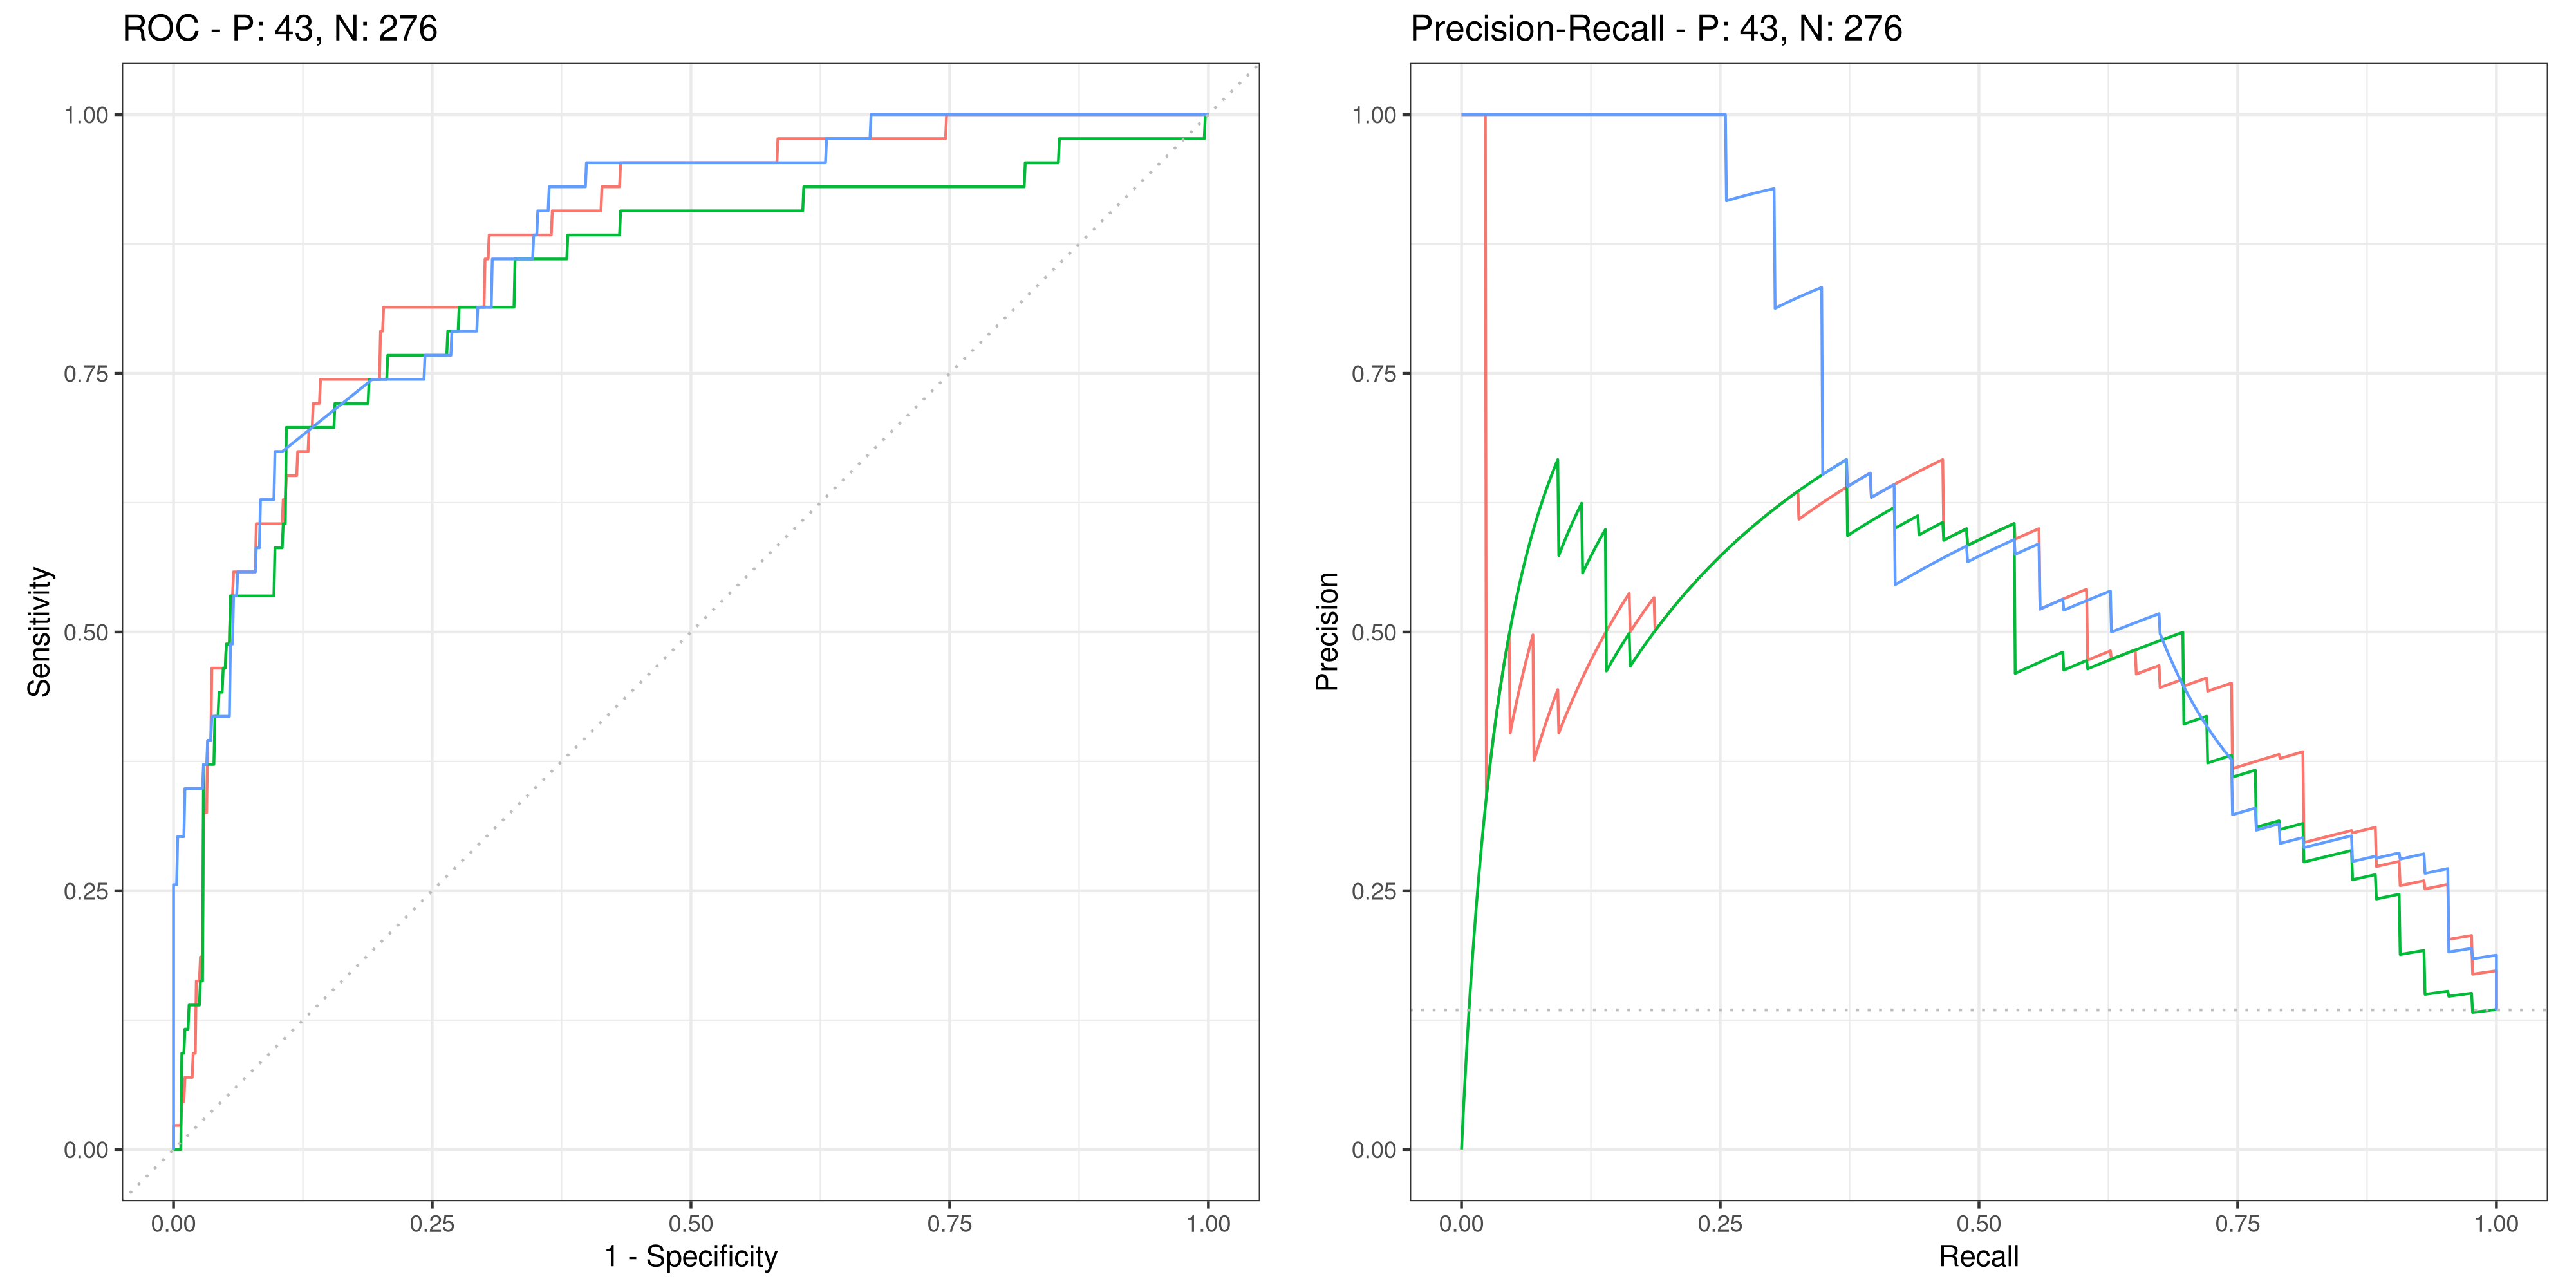
\includegraphics[width=\linewidth]{images/roc/no-outliers/kernel/z-score.png}
    }
    \quad
    \subfloat[Standardizzazione + PCA]{%
        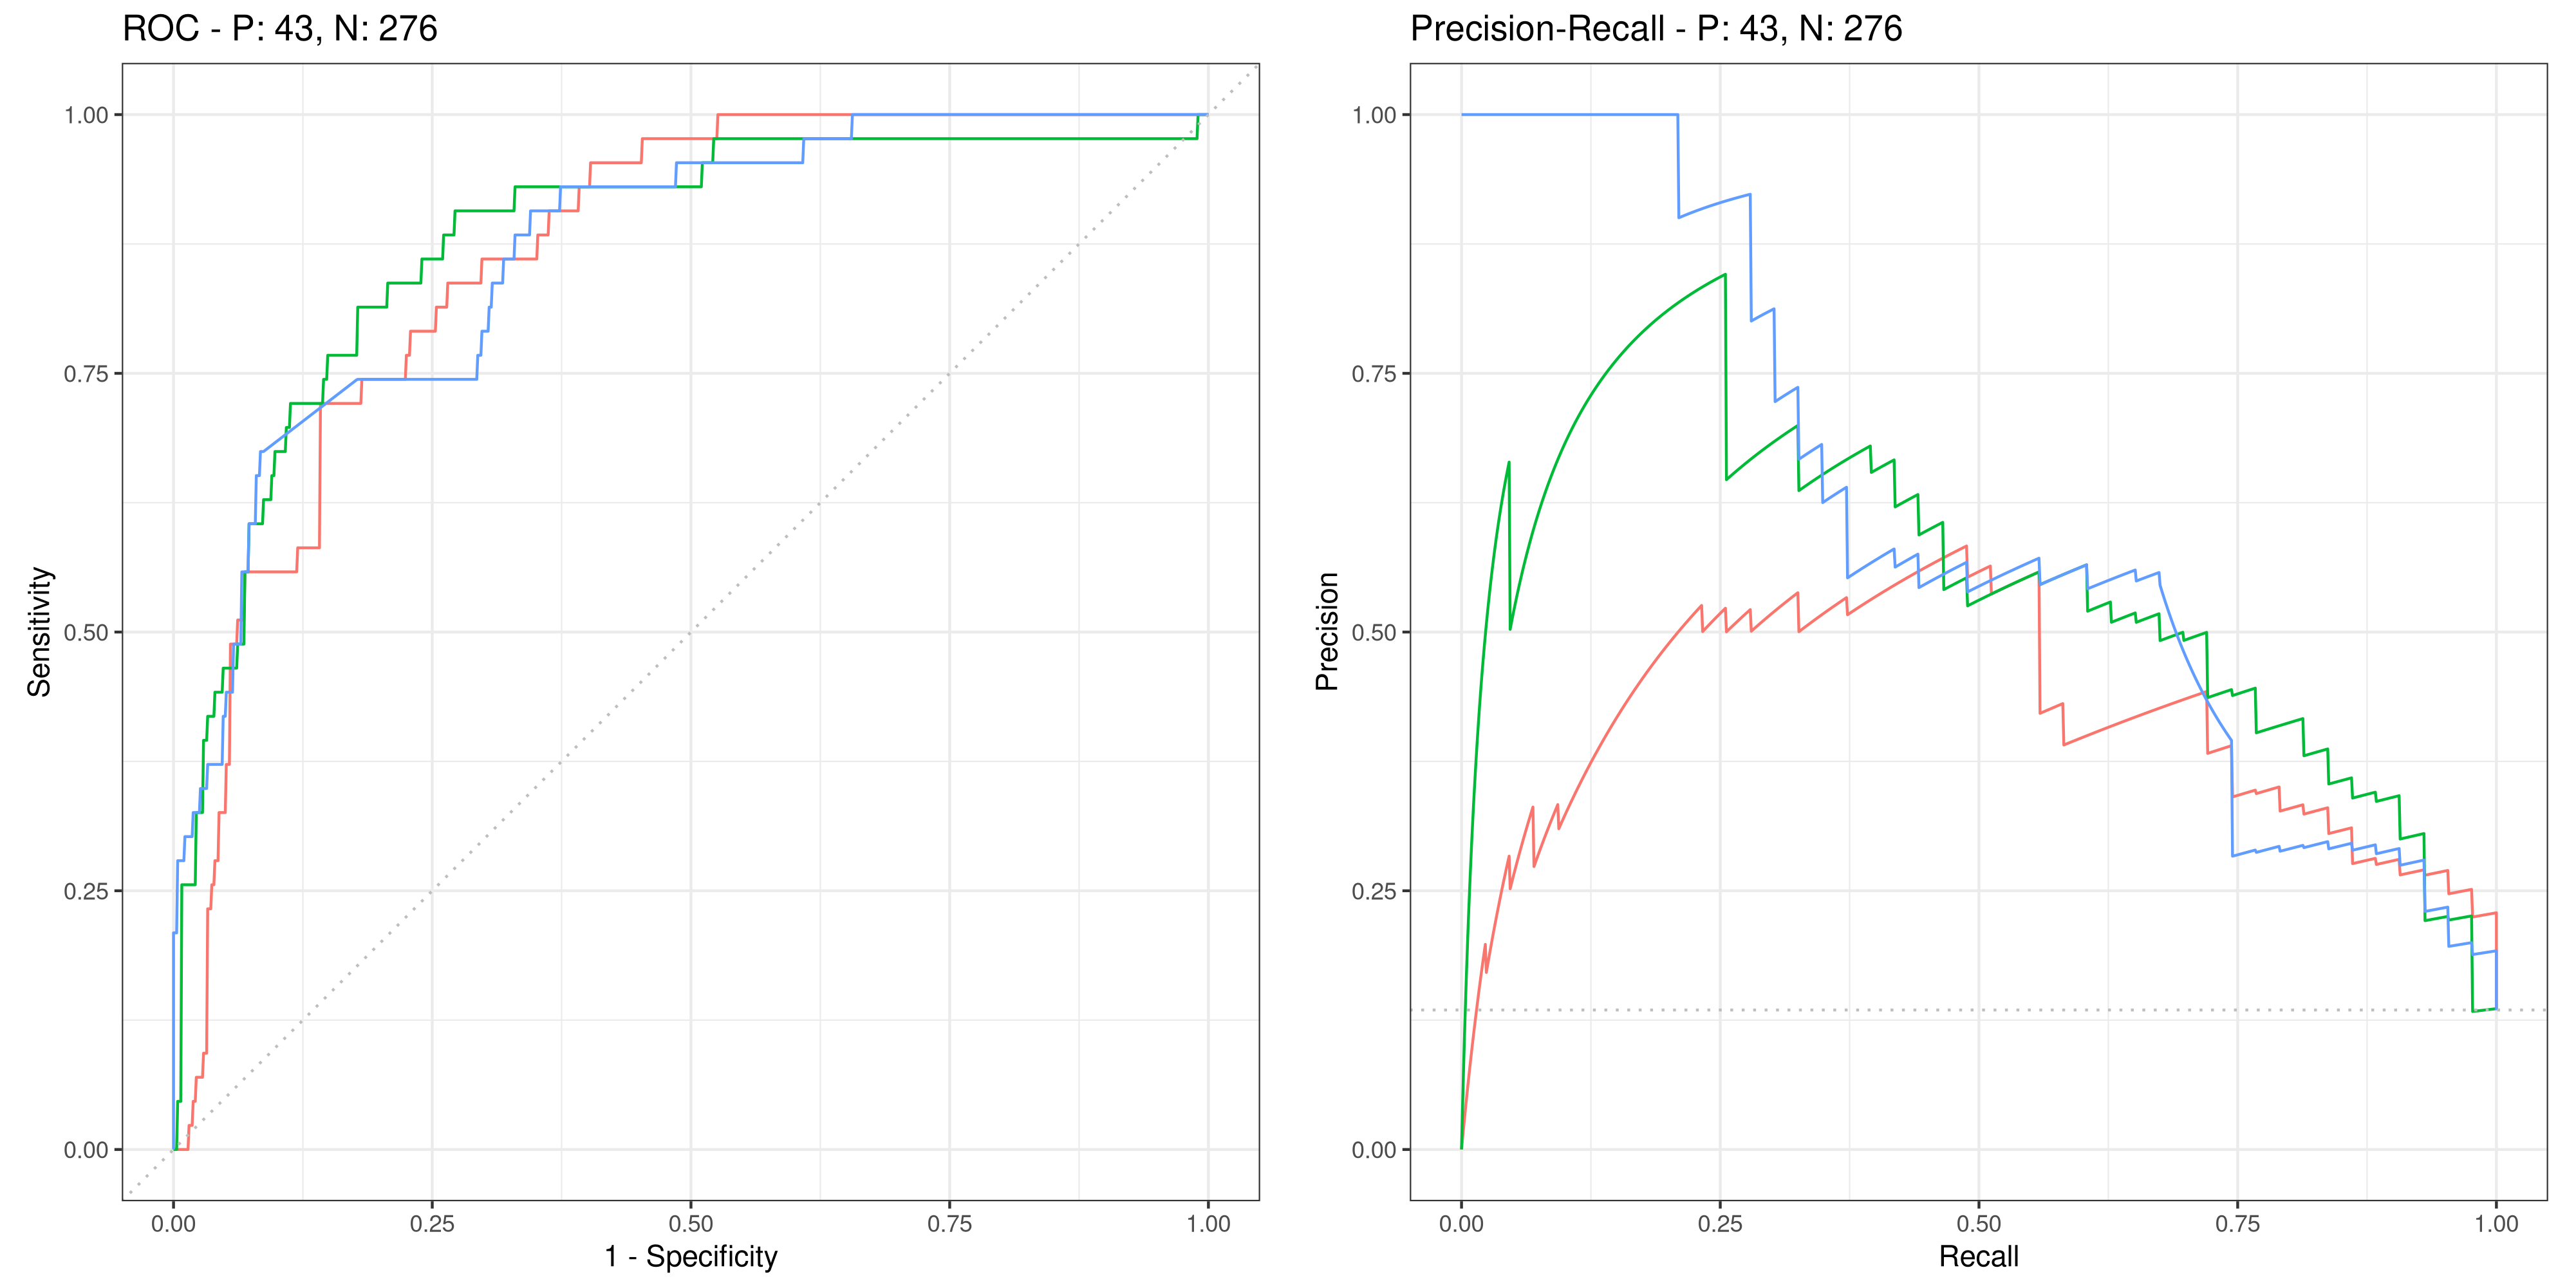
\includegraphics[width=\linewidth]{images/roc/no-outliers/kernel/pca.png}
    }

    \label{fig:roc_svm}
    \caption{Curve ROC e PRC per i diversi kernel (lineare: rosso, polinomiale: verde, radiale: blu) sul testset senza outliers}
\end{figure}

\newpage

\noindent
Riassumendo nella seguente tabella è possibile vedere come il kernel radiale superi gli altri kernel mantenendo gli outliers, mentre effettuando la rimozione con il kernel polinomiale si assumono valori più alti di F1 e Recall.
E' possibile notare che la ROC e la PRC si abbassano drasticamente rimuovendo gli outliers.
Possiamo quindi concludere che l'SVM con kernel radiale, a prescindere dal pre processing, risulti il modello migliore nella maggioranza dei casi analizzati.

\begin{table}[H]
\centering
\resizebox{\textwidth}{!}{%
\begin{tabular}{@{}ccccccccc@{}}
\toprule
\textbf{Kernel} & \textbf{Overall Accuracy} & \textbf{Precision} & \textbf{Recall} & \textbf{F1} & \textbf{ROC AUC} & \textbf{PRC AUC} & \textbf{95\% CI} & \textbf{P-Value} \\ \midrule
lineare & 0.8652 & NA & 0 & NA & 0.8604651 & 0.4288328 & (0.8228, 0.9007) & 0.5405 \\
polinomiale & 0.8746 & 0.57895 & 0.25581 & 0.35484 & 0.8795079 & 0.5608824 & (0.8332, 0.9089) & 0.3471558 \\
radiale & \textbf{0.9122} & \textbf{0.94118} & \textbf{0.37209} & \textbf{0.53333} & \textbf{0.9313279} & \textbf{0.7520759} & (0.8756, 0.9409) & 0.006404 \\ \bottomrule
\end{tabular}%
}
\caption{Risultati dei diversi kernel sul testset con Standardizzazione}
\label{tab:my-table}
\end{table}

\begin{table}[H]
\centering
\resizebox{\textwidth}{!}{%
\begin{tabular}{@{}ccccccccc@{}}
\toprule
\textbf{Kernel} & \textbf{Overall Accuracy} & \textbf{Precision} & \textbf{Recall} & \textbf{F1} & \textbf{ROC AUC} & \textbf{PRC AUC} & \textbf{95\% CI} & \textbf{P-Value} \\ \midrule
lineare & 0.8652 & NA & 0 & NA & 0.8547354 & 0.5011905 & (0.8228, 0.9007) & 0.5405 \\
polinomiale & 0.8715 & 0.54545 & 0.27907 & 0.36923 & 0.8844793 & 0.5368917 & (0.8297, 0.9062) & 0.410227 \\
radiale & \textbf{0.9122} & \textbf{0.94118} & \textbf{0.37209} & \textbf{0.53333} & \textbf{0.9469161} & \textbf{0.7732596} & (0.8756, 0.9409) & 0.006404 \\ \bottomrule
\end{tabular}%
}
\caption{Risultati dei diversi kernel sul testset con Standardizzazione + PCA}
\label{tab:my-table}
\end{table}

\begin{table}[H]
\centering
\resizebox{\textwidth}{!}{%
\begin{tabular}{@{}ccccccccc@{}}
\toprule
\textbf{Kernel} & \textbf{Overall Accuracy} & \textbf{Precision} & \textbf{Recall} & \textbf{F1} & \textbf{ROC AUC} & \textbf{PRC AUC} & \textbf{95\% CI} & \textbf{P-Value} \\ \midrule
lineare & 0.8652 & NA & 0 & NA & 0.8681328 & 0.4870888 & (0.8228, 0.9007) & 0.5405 \\
polinomiale & 0.884 & 0.59375 & \textbf{0.44186} & \textbf{0.50667} & 0.8313953 & 0.4587525 & (0.8437, 0.917) & 0.1845 \\
radiale & \textbf{0.8997} & \textbf{0.92308} & 0.27907 & 0.42857 & \textbf{0.8711662} & \textbf{0.6230968} & (0.8613, 0.9304) & 0.03864 \\ \bottomrule
\end{tabular}%
}
\caption{Risultati dei diversi kernel sul testset con Standardizzazione e rimozione outliers}
\label{tab:my-table}
\end{table}

\begin{table}[H]
\centering
\resizebox{\textwidth}{!}{%
\begin{tabular}{@{}ccccccccc@{}}
\toprule
\textbf{Kernel} & \textbf{Overall Accuracy} & \textbf{Precision} & \textbf{Recall} & \textbf{F1} & \textbf{ROC AUC} & \textbf{PRC AUC} & \textbf{95\% CI} & \textbf{P-Value} \\ \midrule
lineare & 0.8652 & NA & 0 & NA & 0.8624031 & 0.408548 & (0.8228, 0.9007) & 0.5405 \\
polinomiale & 0.8903 & 0.63333 & \textbf{0.44186} & \textbf{0.52055} & \textbf{0.878244} & 0.5411327 & (0.8507, 0.9224) & 0.10722 \\
radiale & \textbf{0.8934} & \textbf{0.90909} & 0.23256 & 0.37037 & 0.8684277 & \textbf{0.6079154} & (0.8543, 0.9251) & 0.07852 \\ \bottomrule
\end{tabular}%
}
\caption{Risultati dei diversi kernel sul testset con Standardizzazione + PCA e rimozione outliers}
\label{tab:my-table}
\end{table}


\newpage


\section{Confronto fra CART e SVM Radiale}
Così come già mostrato in precedenza per i kernel dell'SVM, vengono ora riportate le performance ottenute dall'SVM radiale e CART. Le metriche considerate sono Accuracy, AUC PRC, F1, Precision e Recall.
Da essi è possibile notare come, a parte il caso [\ref{fig:a}], l'SVM raggiunga i risultati migliori nella maggioranza dei casi.
Nel caso [\ref{fig:a}], invece è difficile dire quale dei due modelli sia il migliore dal momento che i risultati sono molto simili.


\begin{figure}[H]
    \centering

    \subfloat[Standardizzazione]{%
       \label{fig:a} 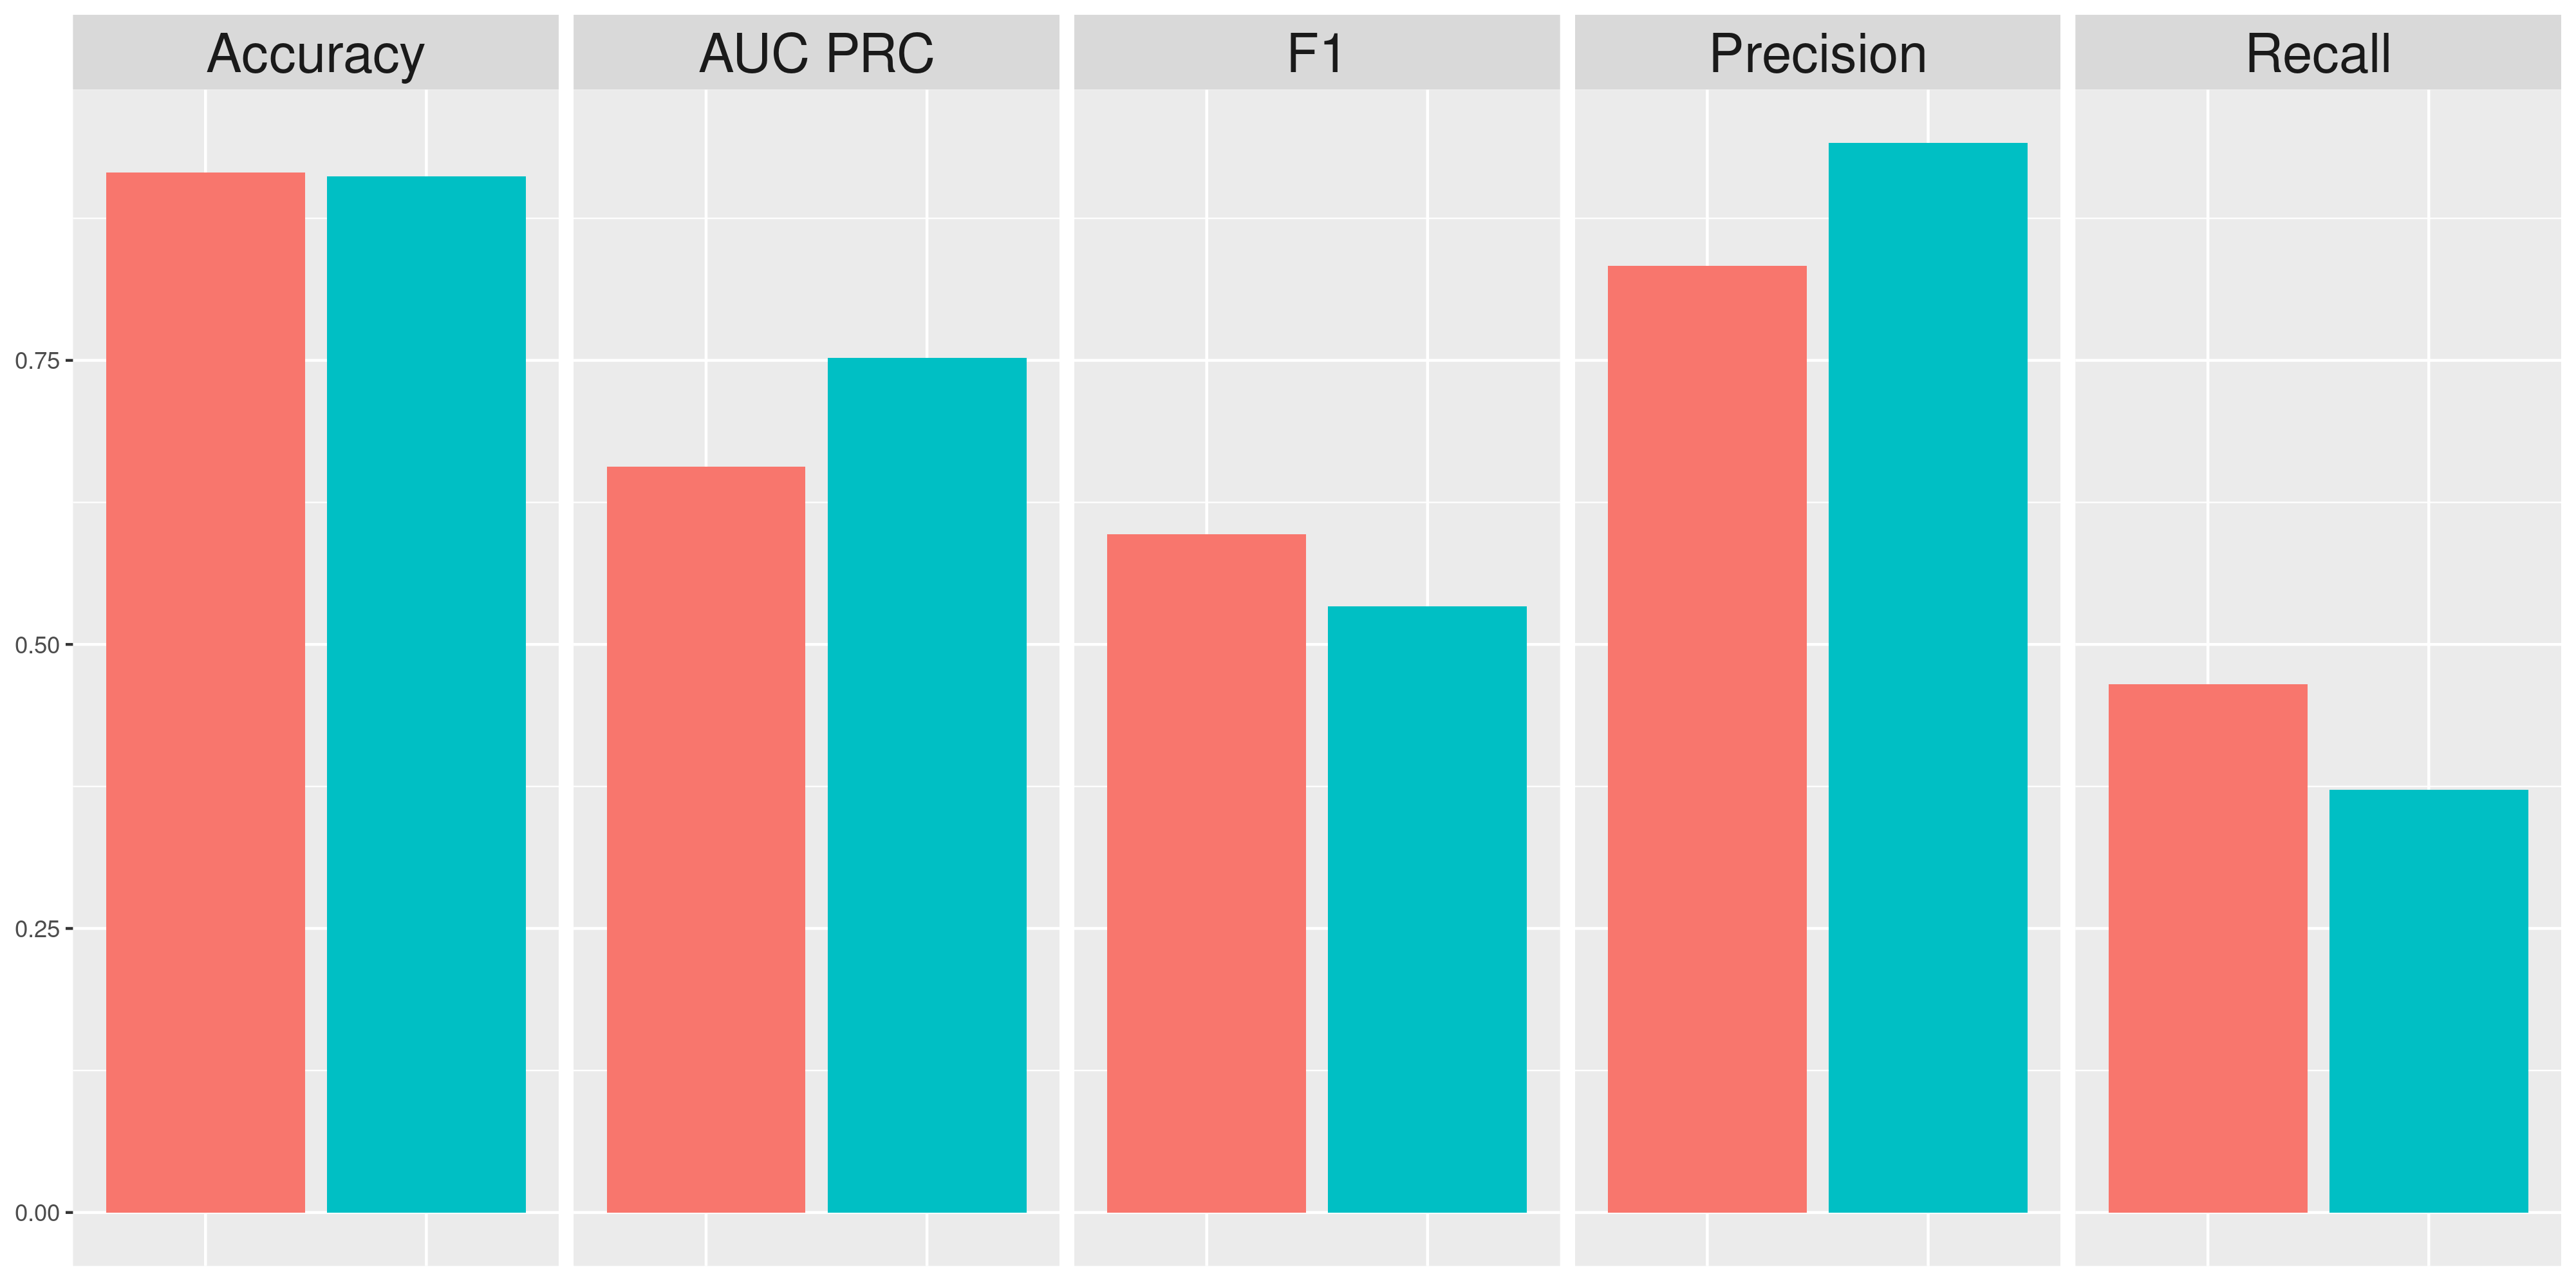
\includegraphics[width=12cm, height=8cm, keepaspectratio]{images/comparison/outliers/z-score_measures.png}
    }
    \quad
    \subfloat[Standardizzazione + PCA]{%
        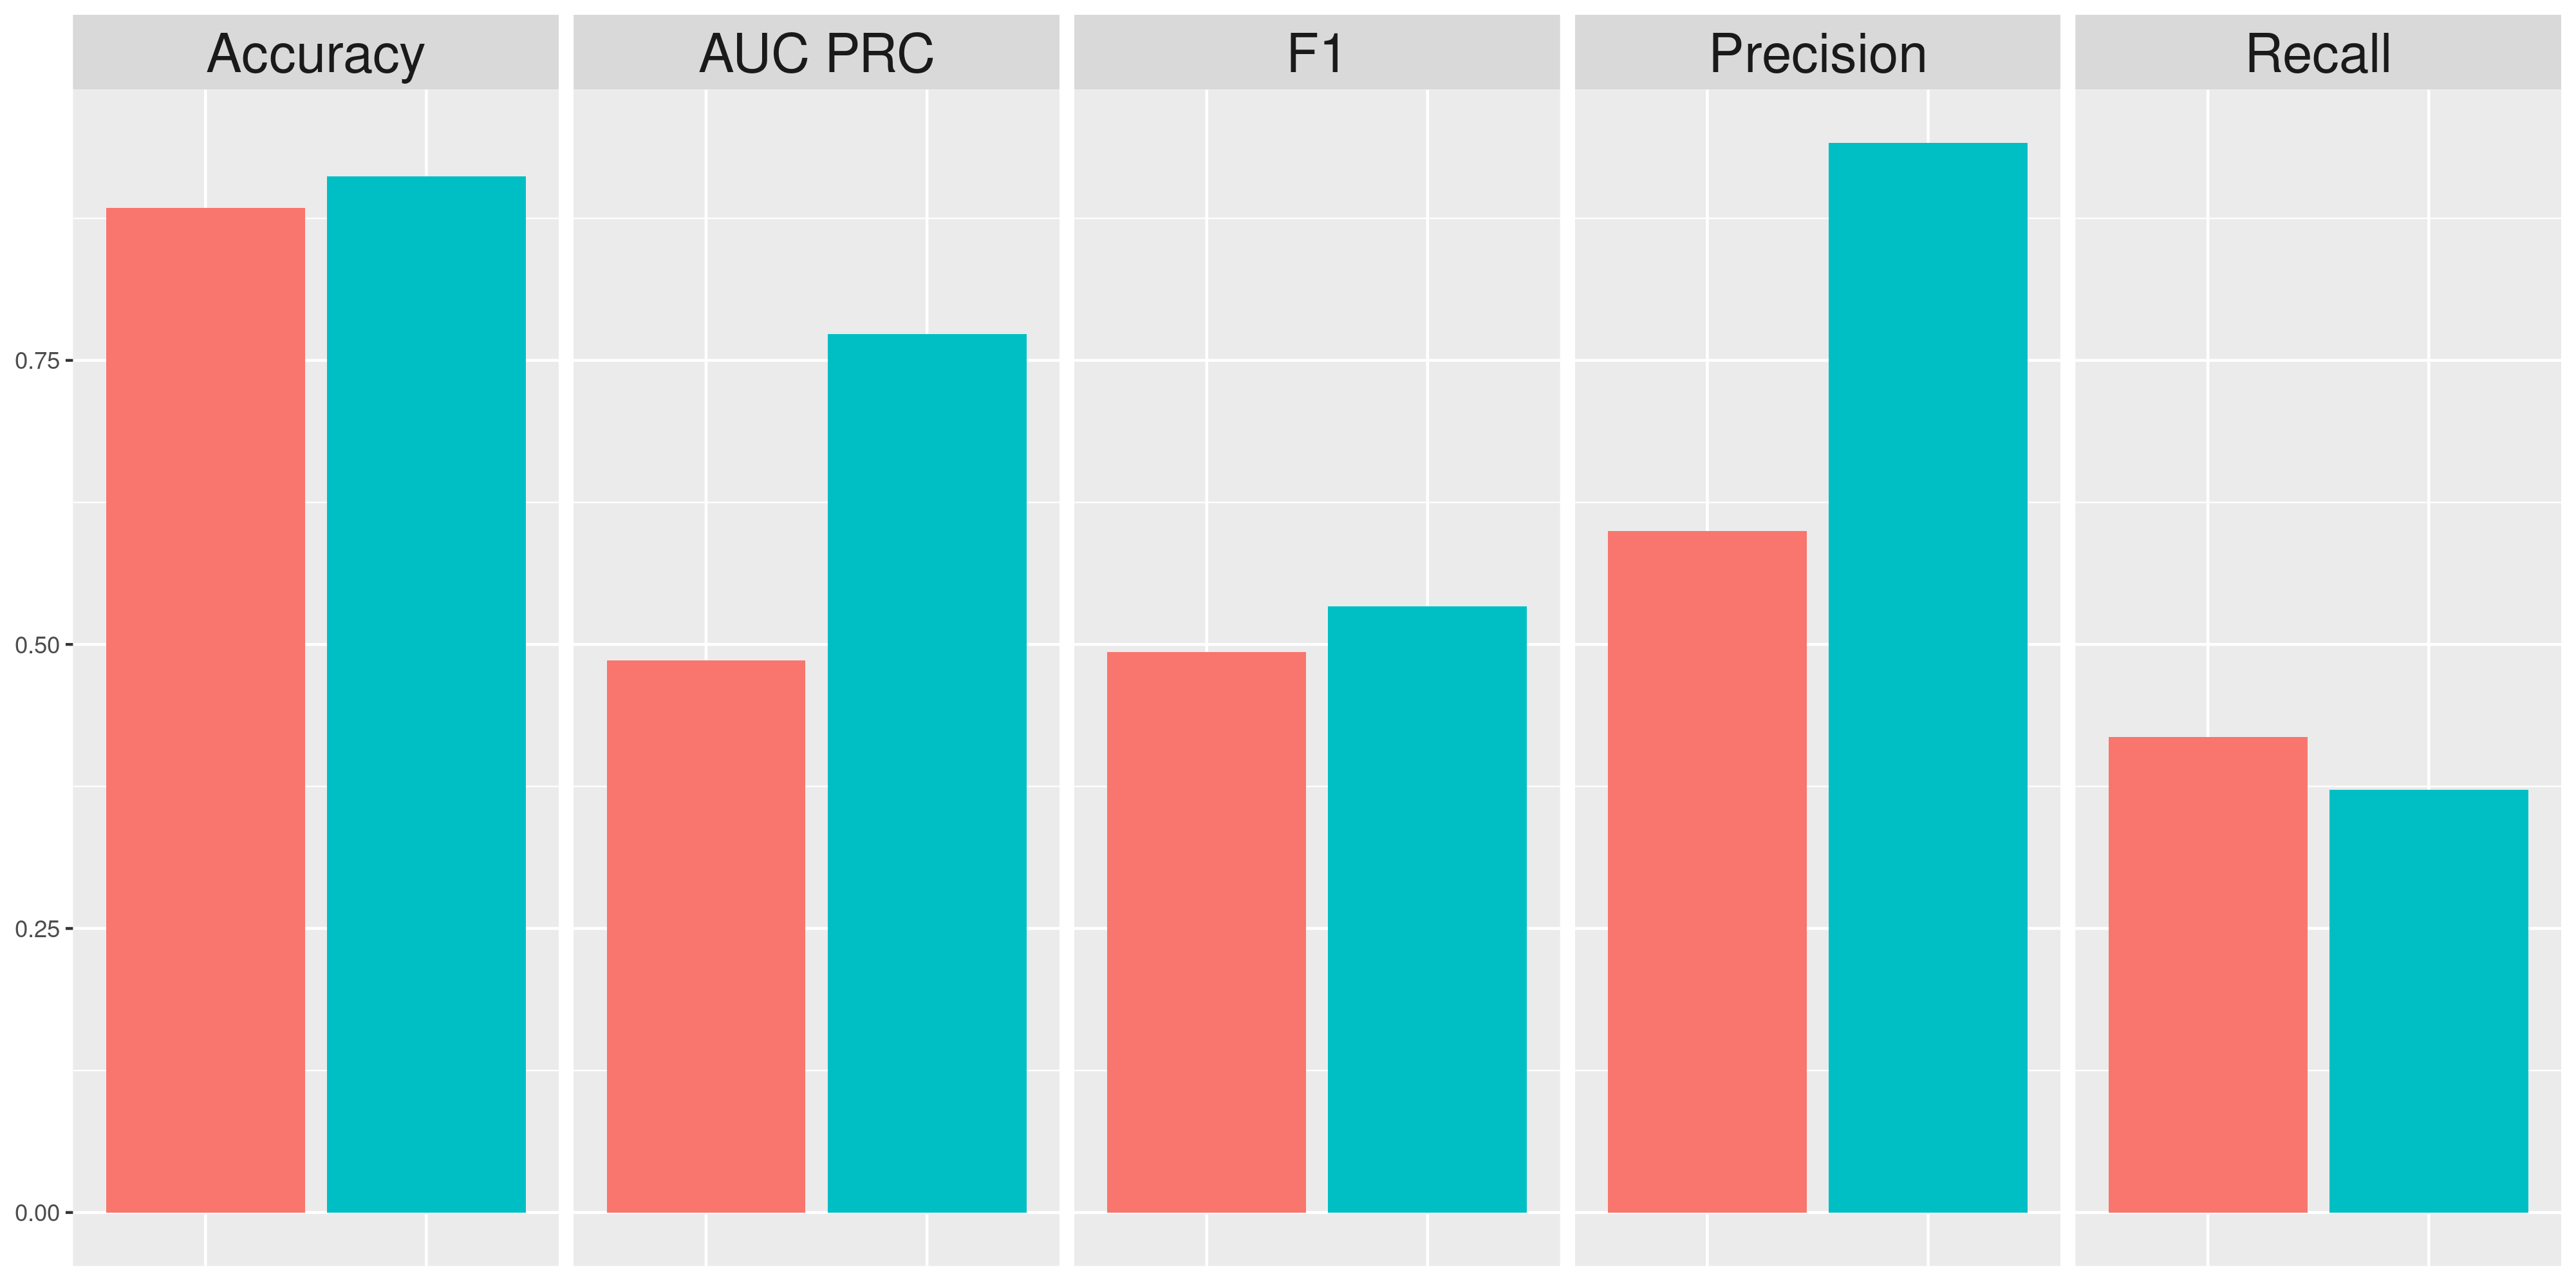
\includegraphics[width=12cm, height=8cm, keepaspectratio]{images/comparison/outliers/pca_measures.png}
    }

    \label{fig:measures_svm_outliers}
     \caption{Risultati dei due modelli (cart: rosso, radiale: blu) sul testset con outliers}
\end{figure}

\begin{figure}[H]
    \centering

    \subfloat[Standardizzazione]{%
        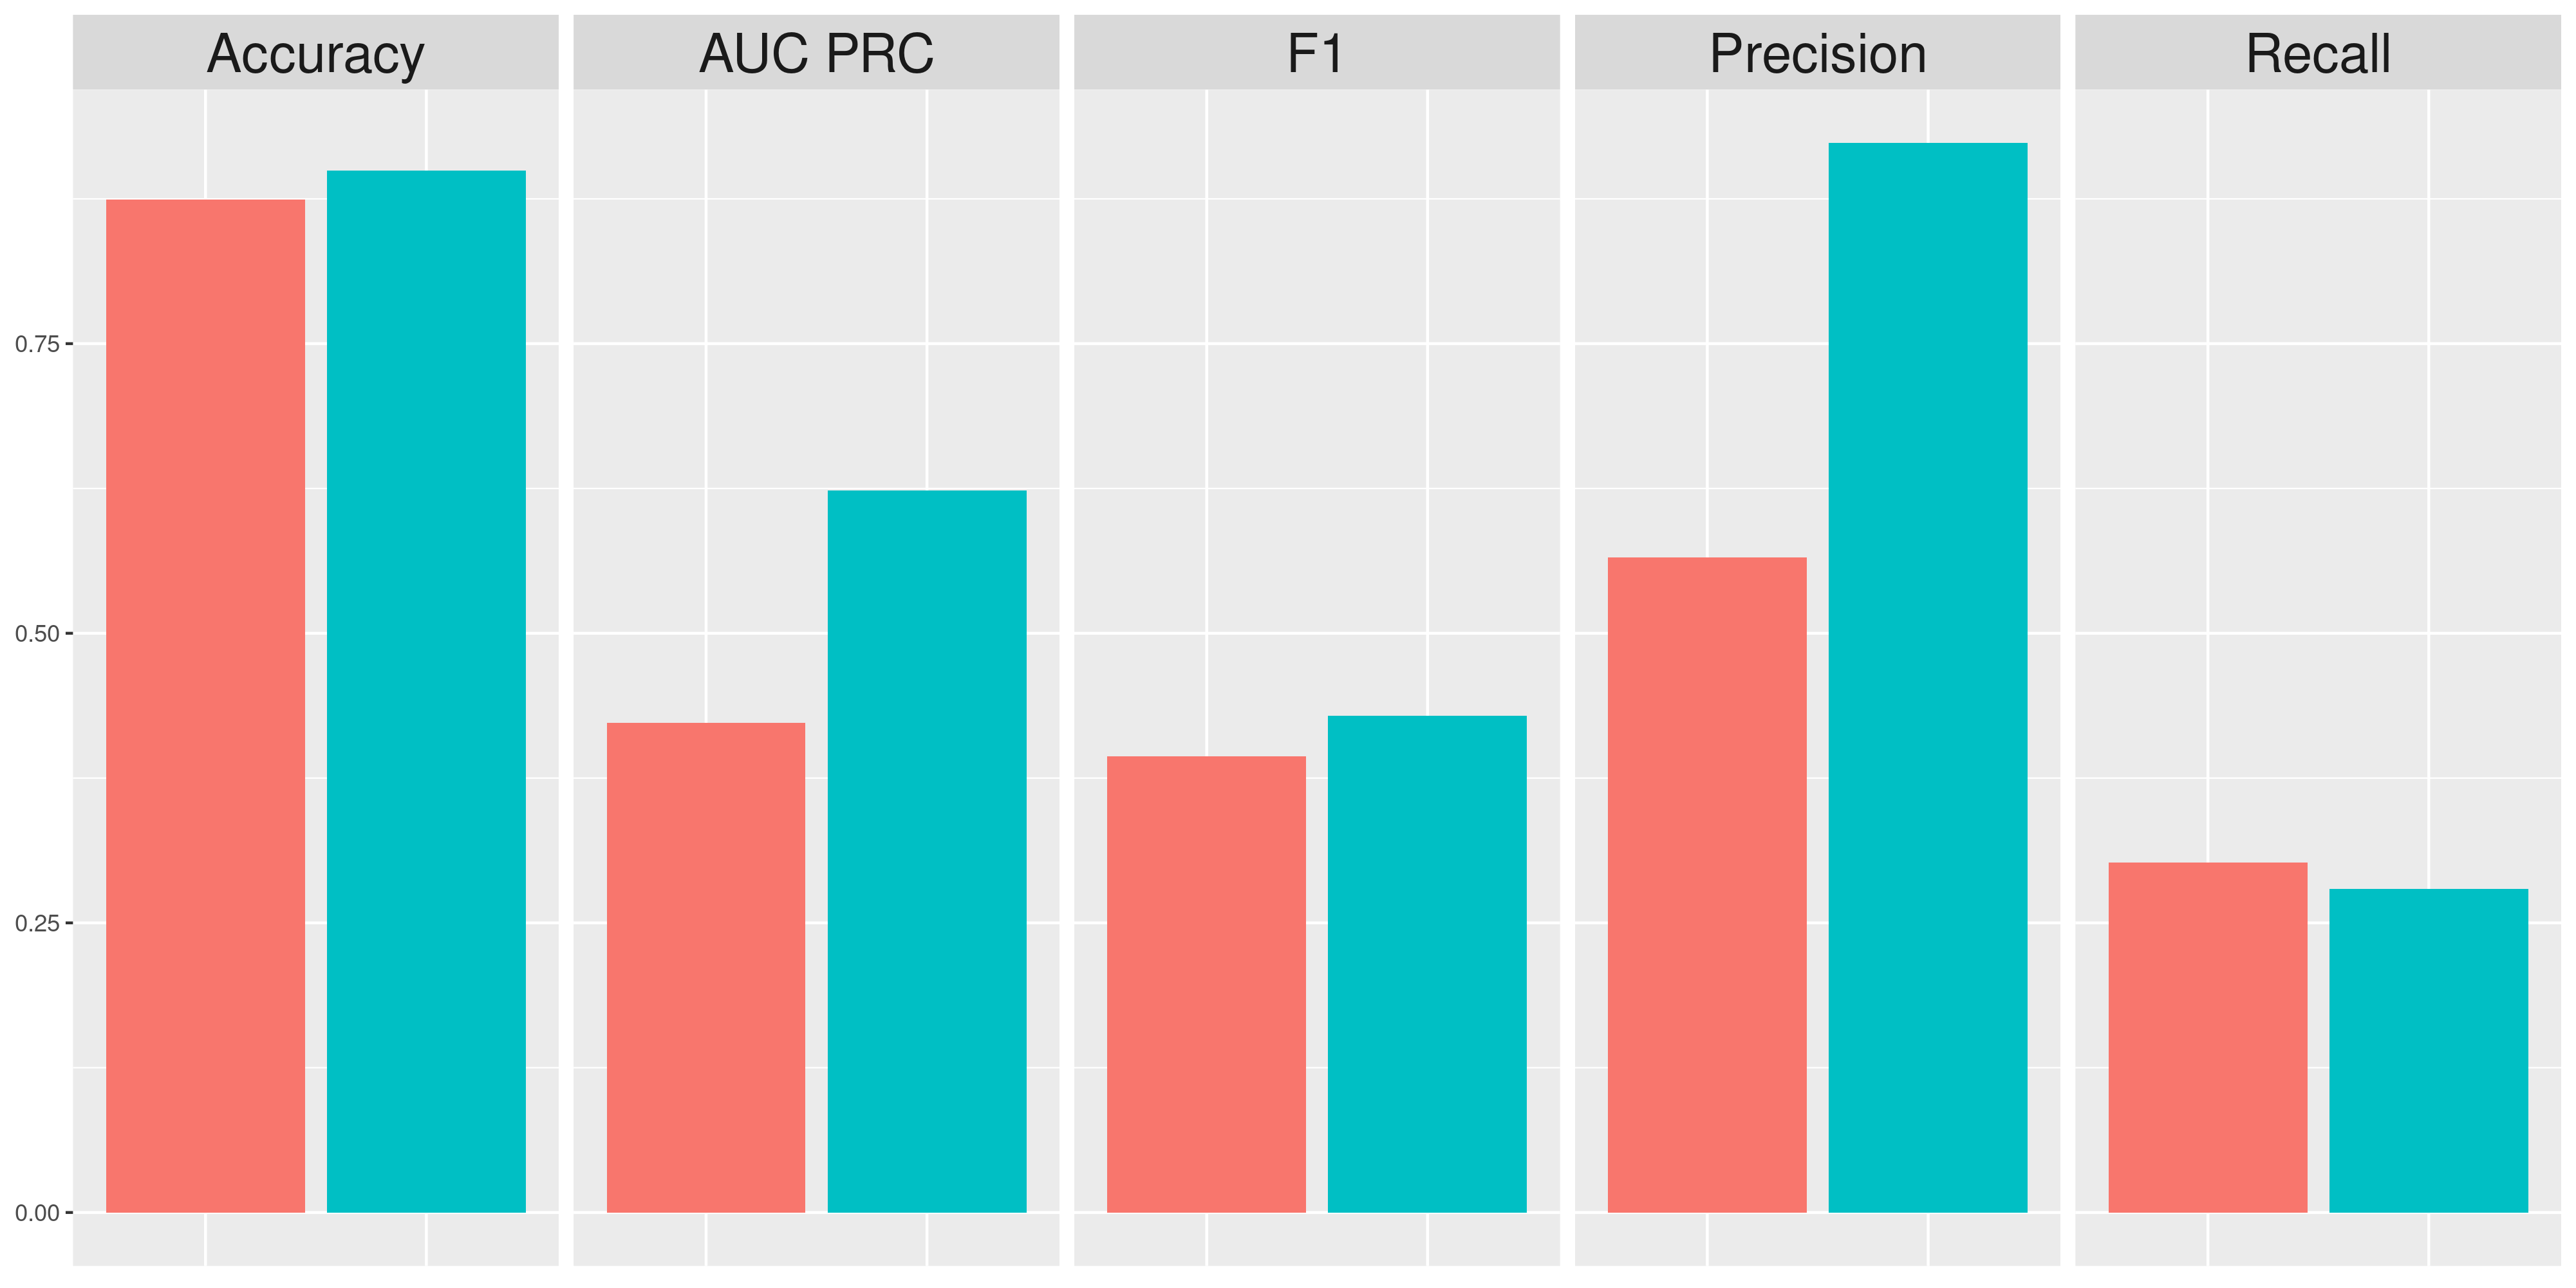
\includegraphics[width=12cm, height=8cm, keepaspectratio]{images/comparison/no-outliers/z-score_measures.png}
    }
    \quad
    \subfloat[Standardizzazione + PCA]{%
        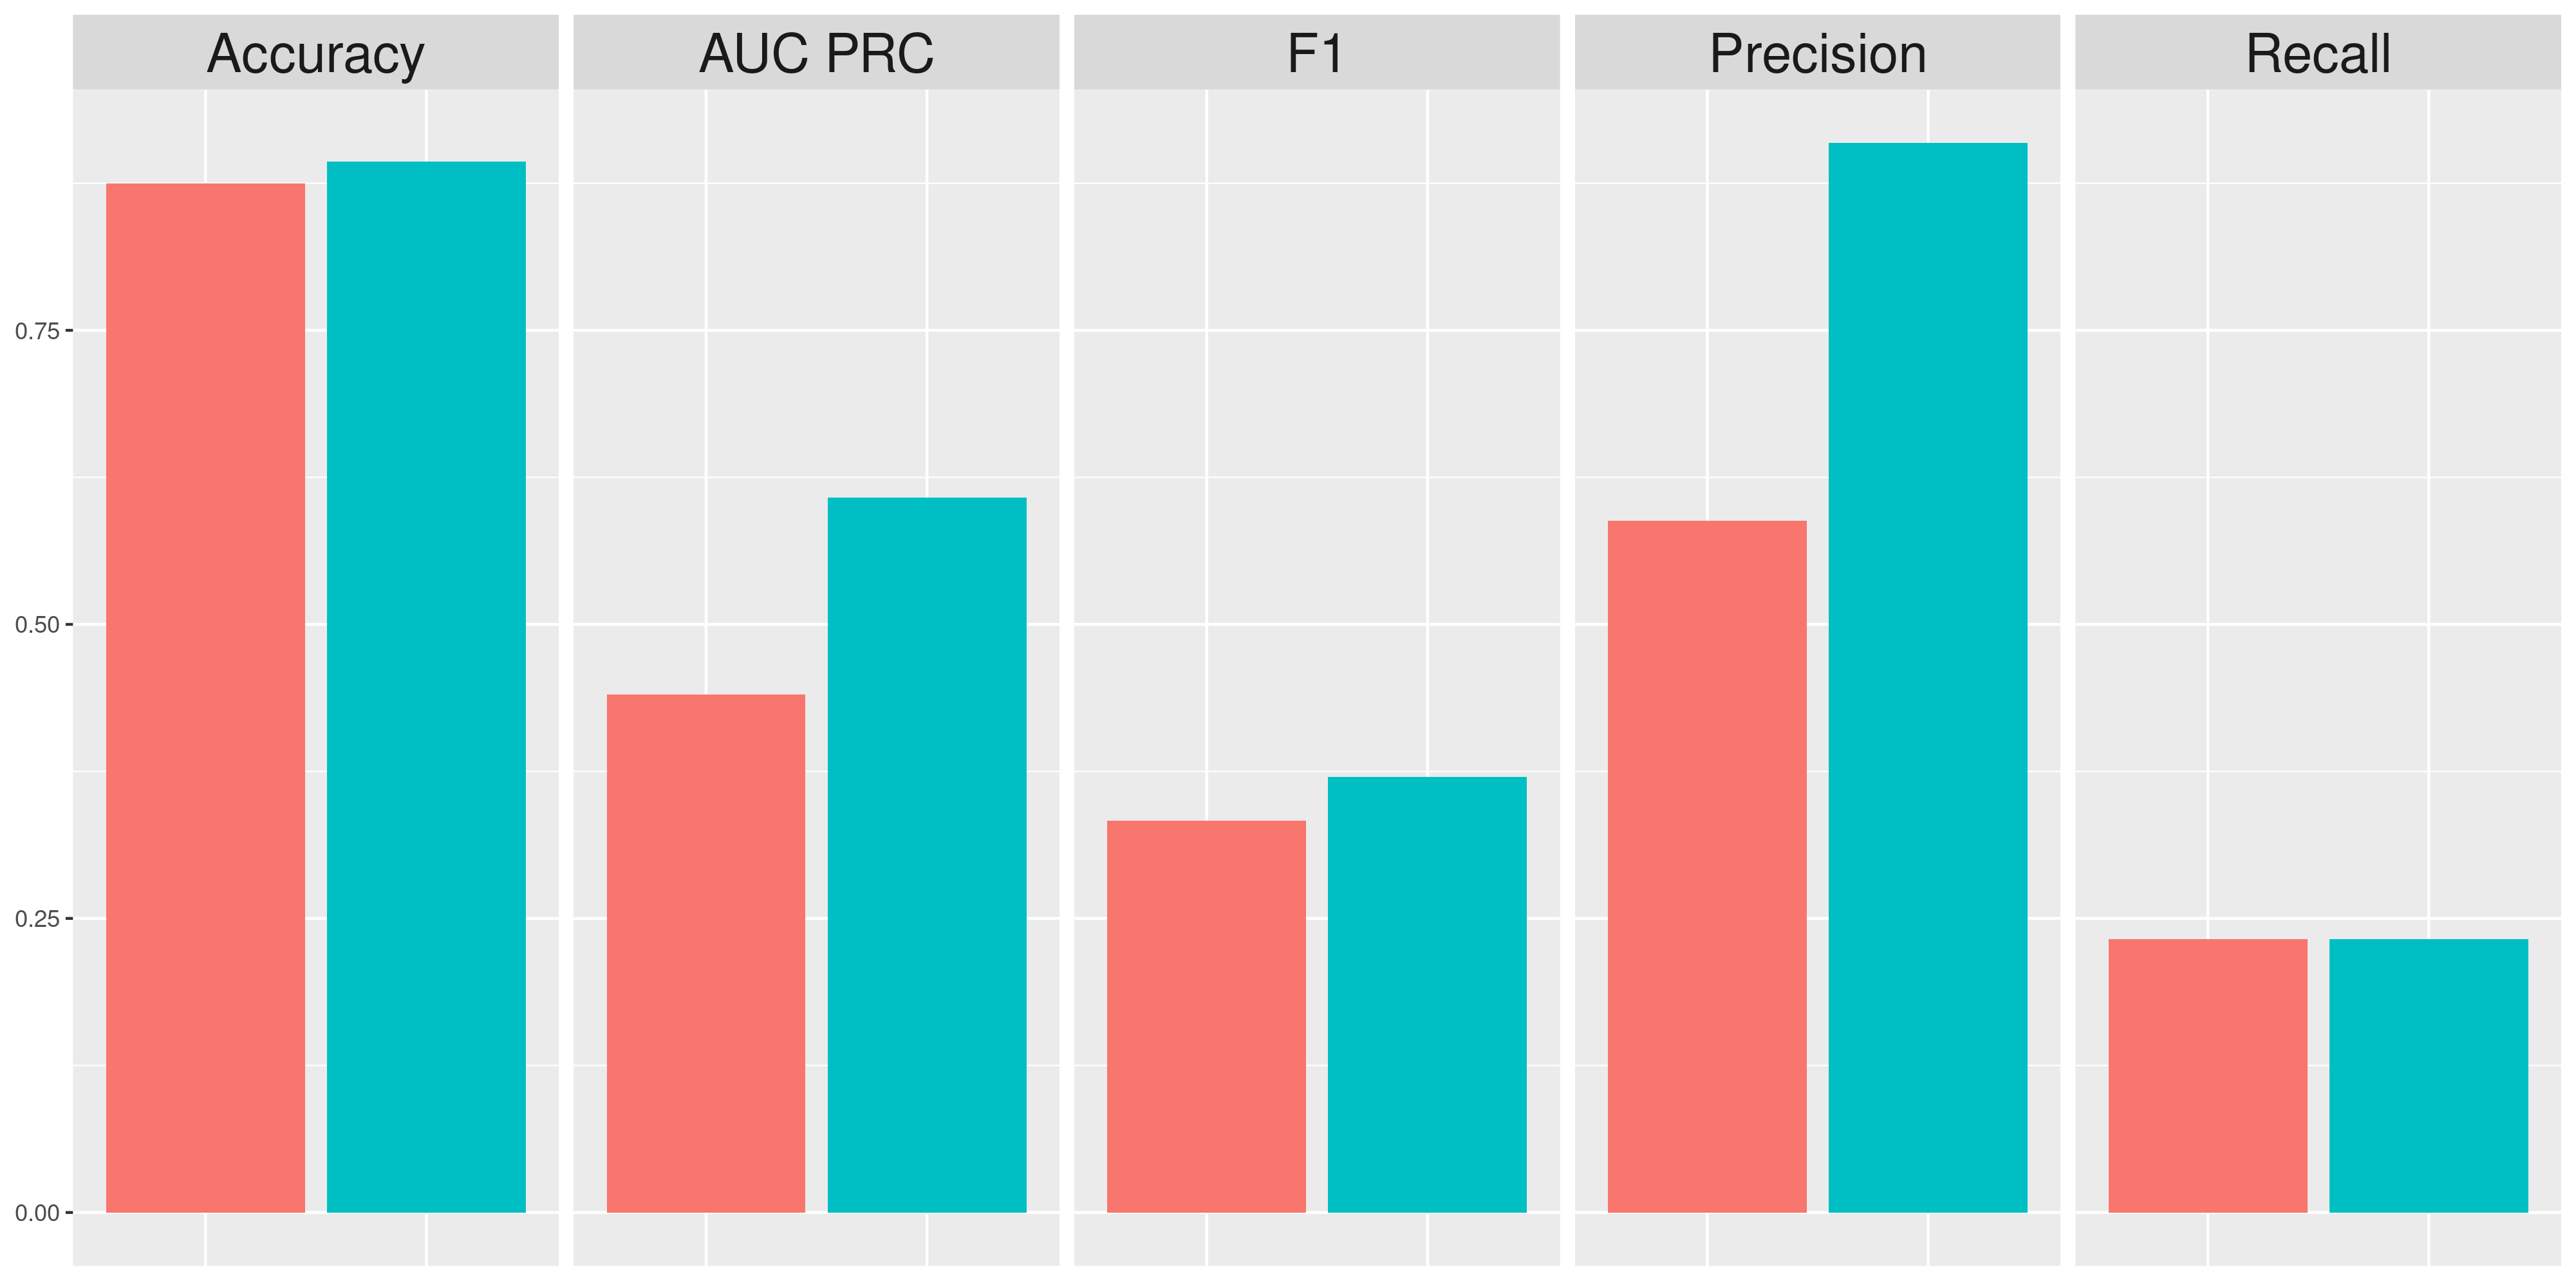
\includegraphics[width=12cm, height=8cm, keepaspectratio]{images/comparison/no-outliers/pca_measures.png}
    }
    
    \label{fig:measures_svm}
    \caption{Risultati dei due modelli (cart: rosso, radiale: blu) sul testset senza outliers}
\end{figure}


\noindent
Osservando le curve ROC e PRC possiamo notare come quelle dell'SVM radiale siano sempre superiori a quelle di CART.
Si riconferma che la rimozione degli outliers peggiora i risultati.
Dal caso [\ref{fig:a-roc}] non è possibile distinguere i risultati dalla curva PRC, per questo sono stati riportati in tabelle i valori di AUC (Area Under The Curve) che confermano che anche in questo caso l'SVM radiale raggiunge risultati migliori.

\newpage

\begin{figure}[H]
    \centering

    \subfloat[Standardizzazione]{%
        \label{fig:a-roc}
        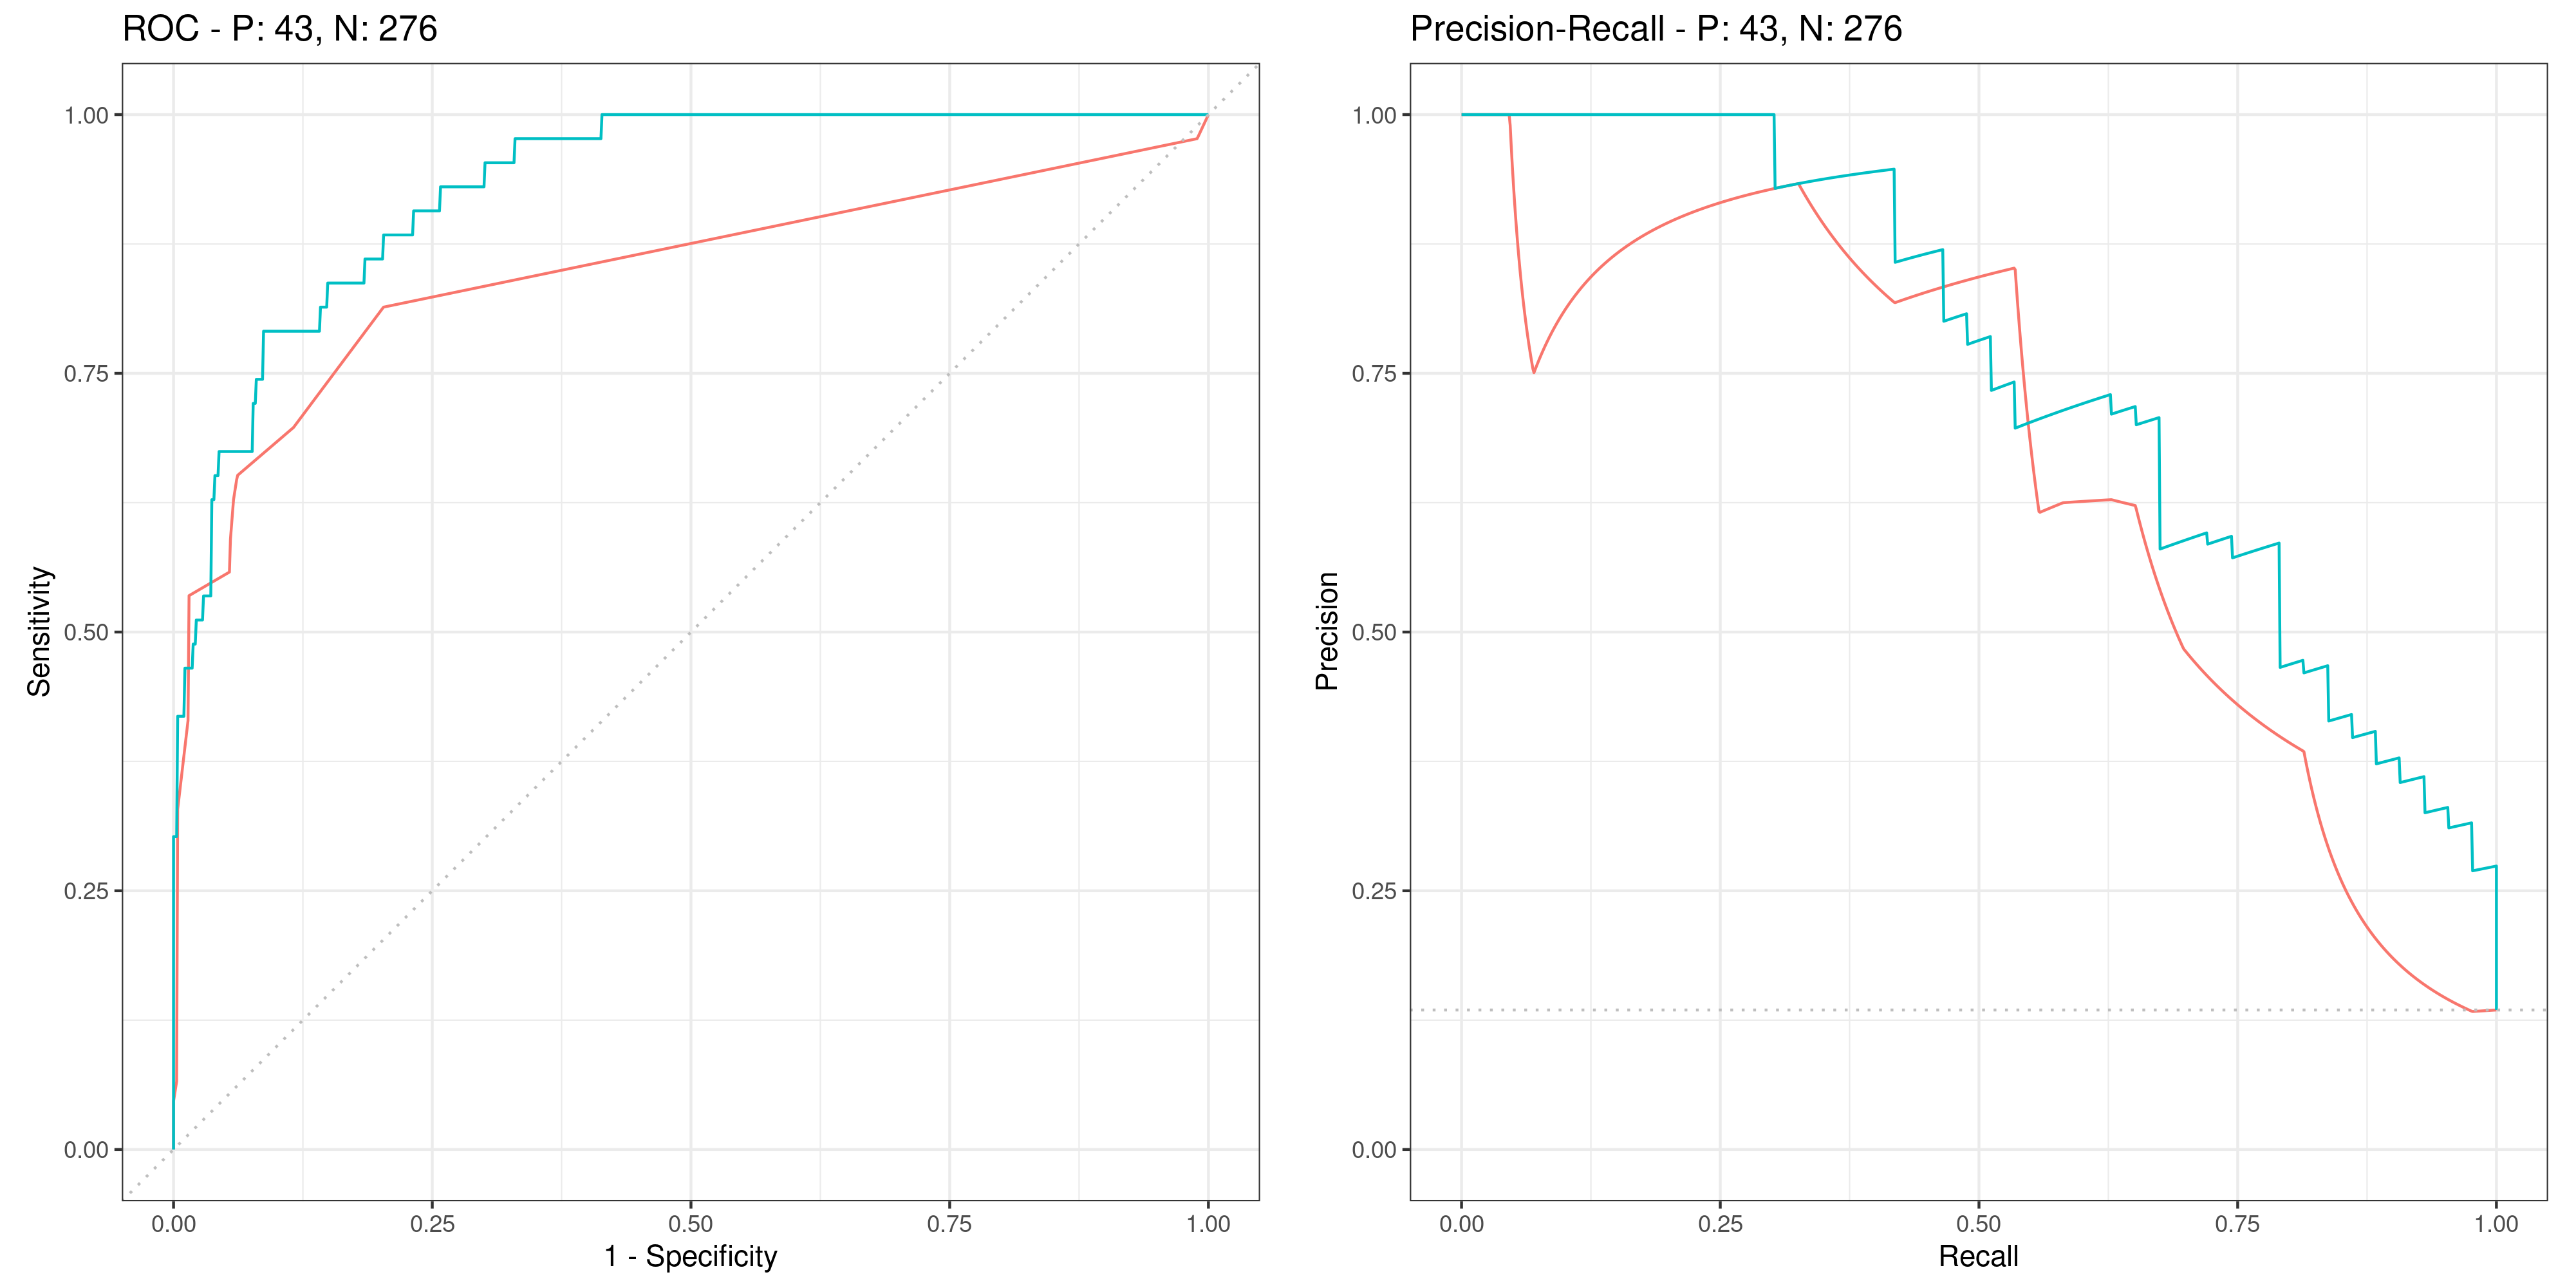
\includegraphics[width=\linewidth]{images/roc/outliers/z-score.png}
    }
    
    \quad
    
    \subfloat[Standardizzazione + PCA]{%
        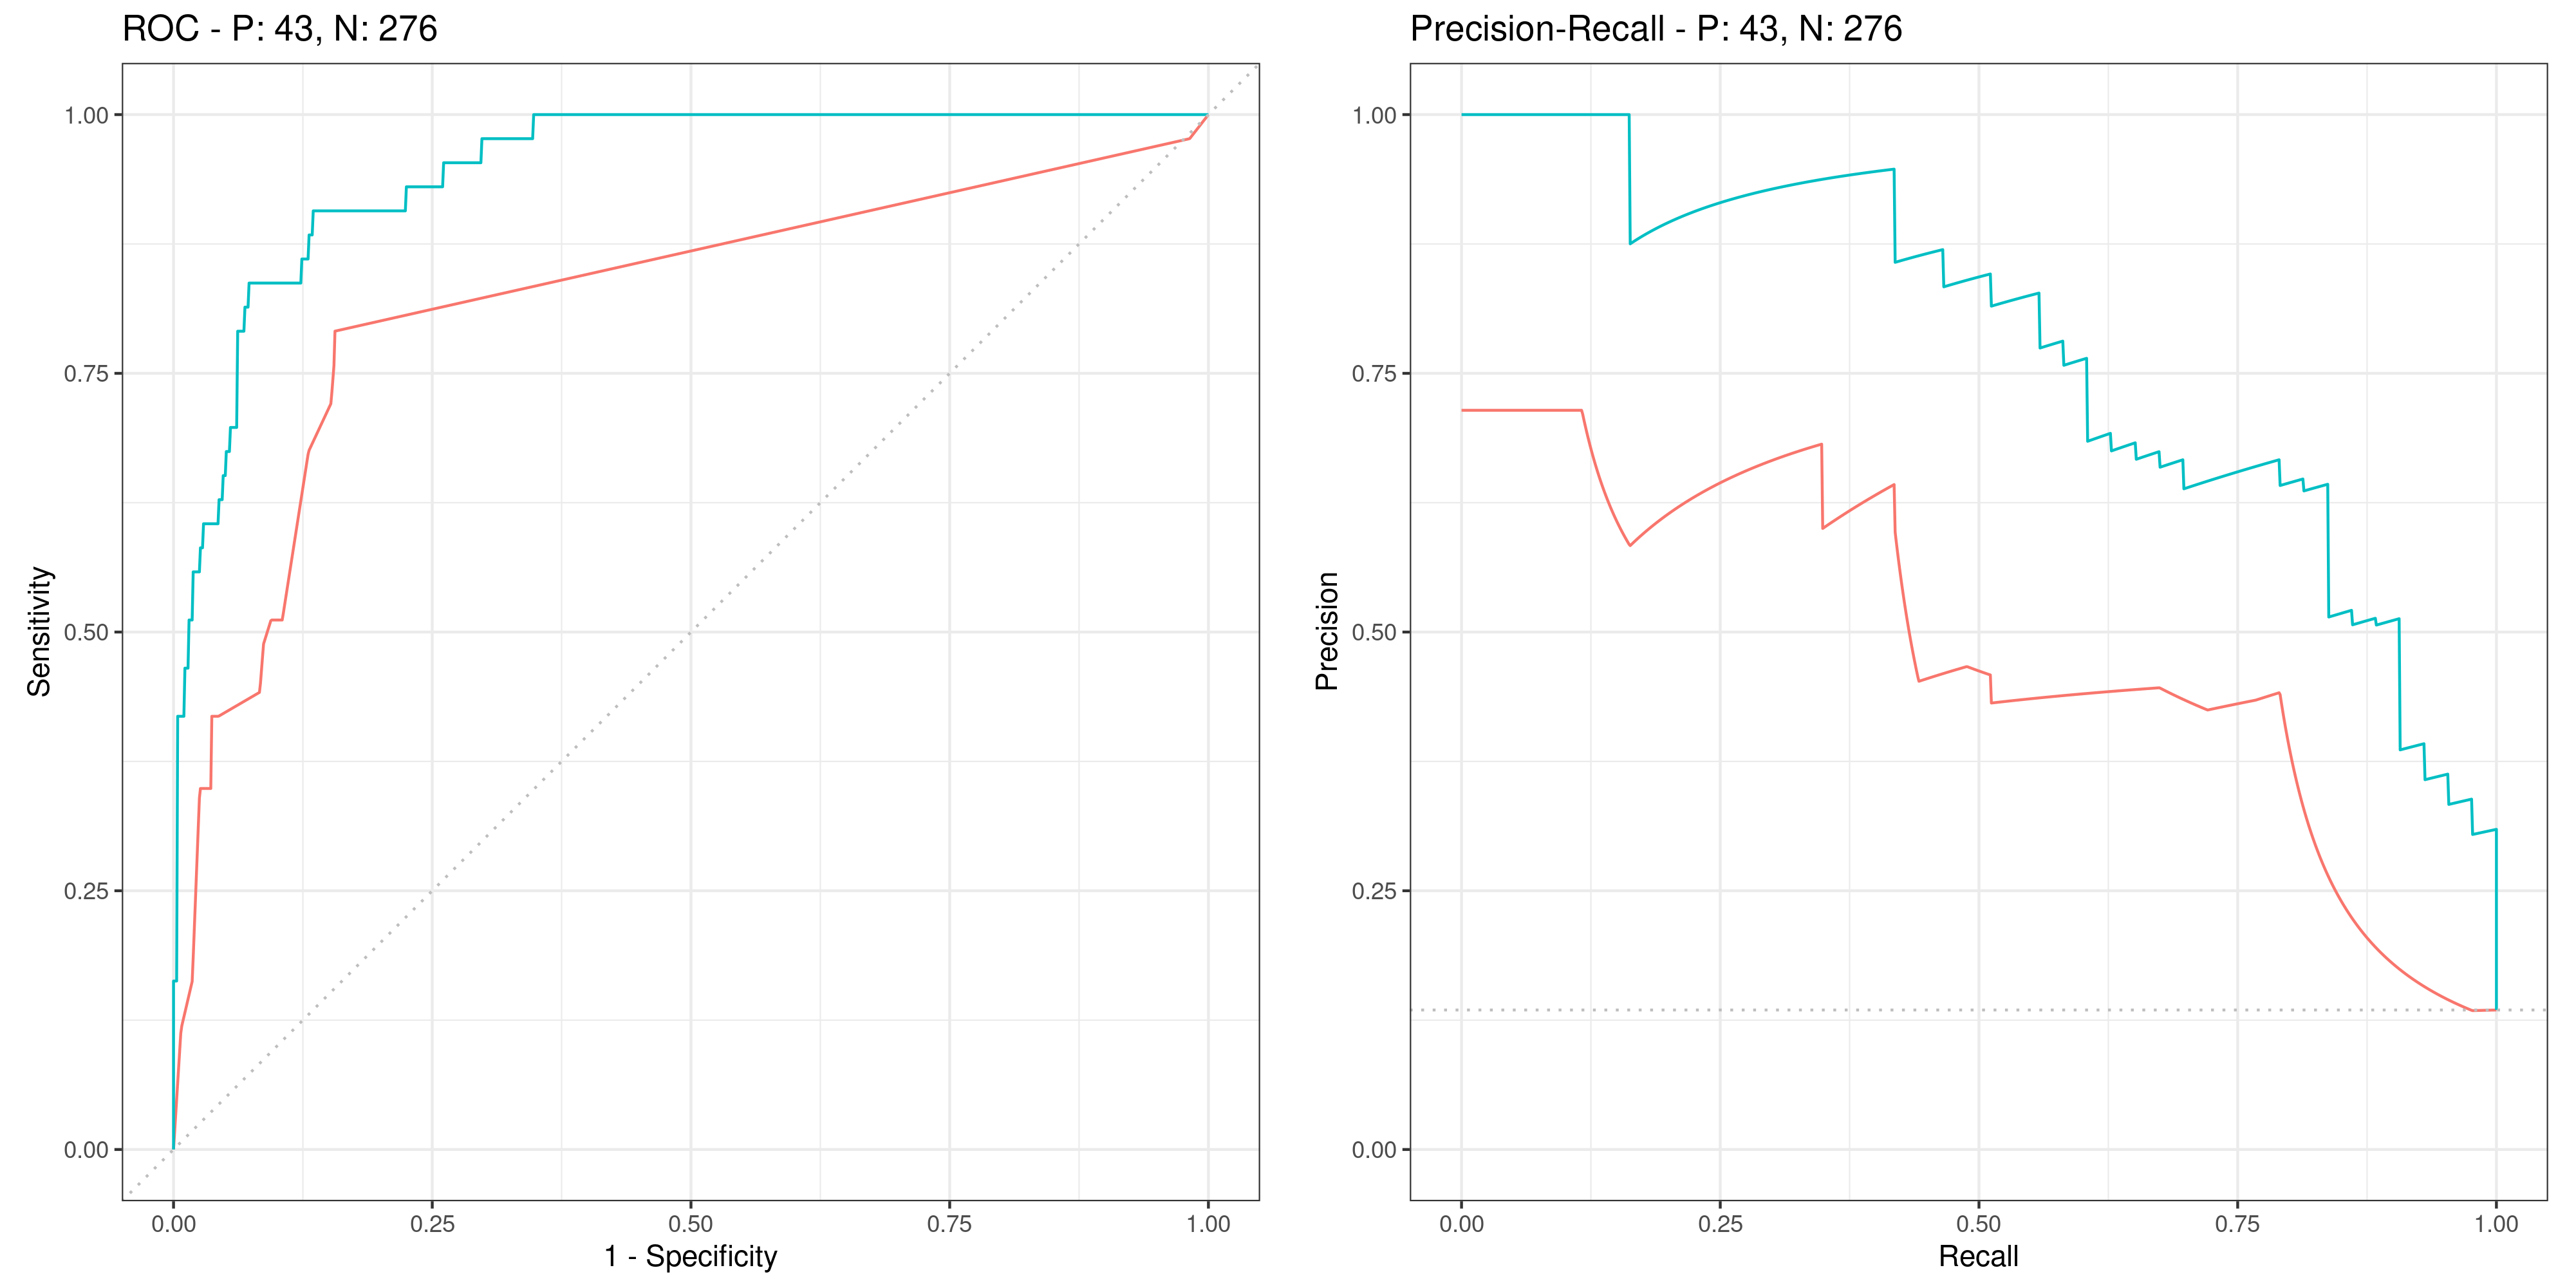
\includegraphics[width=\linewidth]{images/roc/outliers/pca.png}
    }

    \label{fig:roc_prc_svm_outliers}
    \caption{Curve ROC e PRC per i due modelli (cart: rosso, radiale: blu) sul testset con outliers}
\end{figure}

\begin{figure}[H]
    \centering

    \subfloat[Standardizzazione]{%
        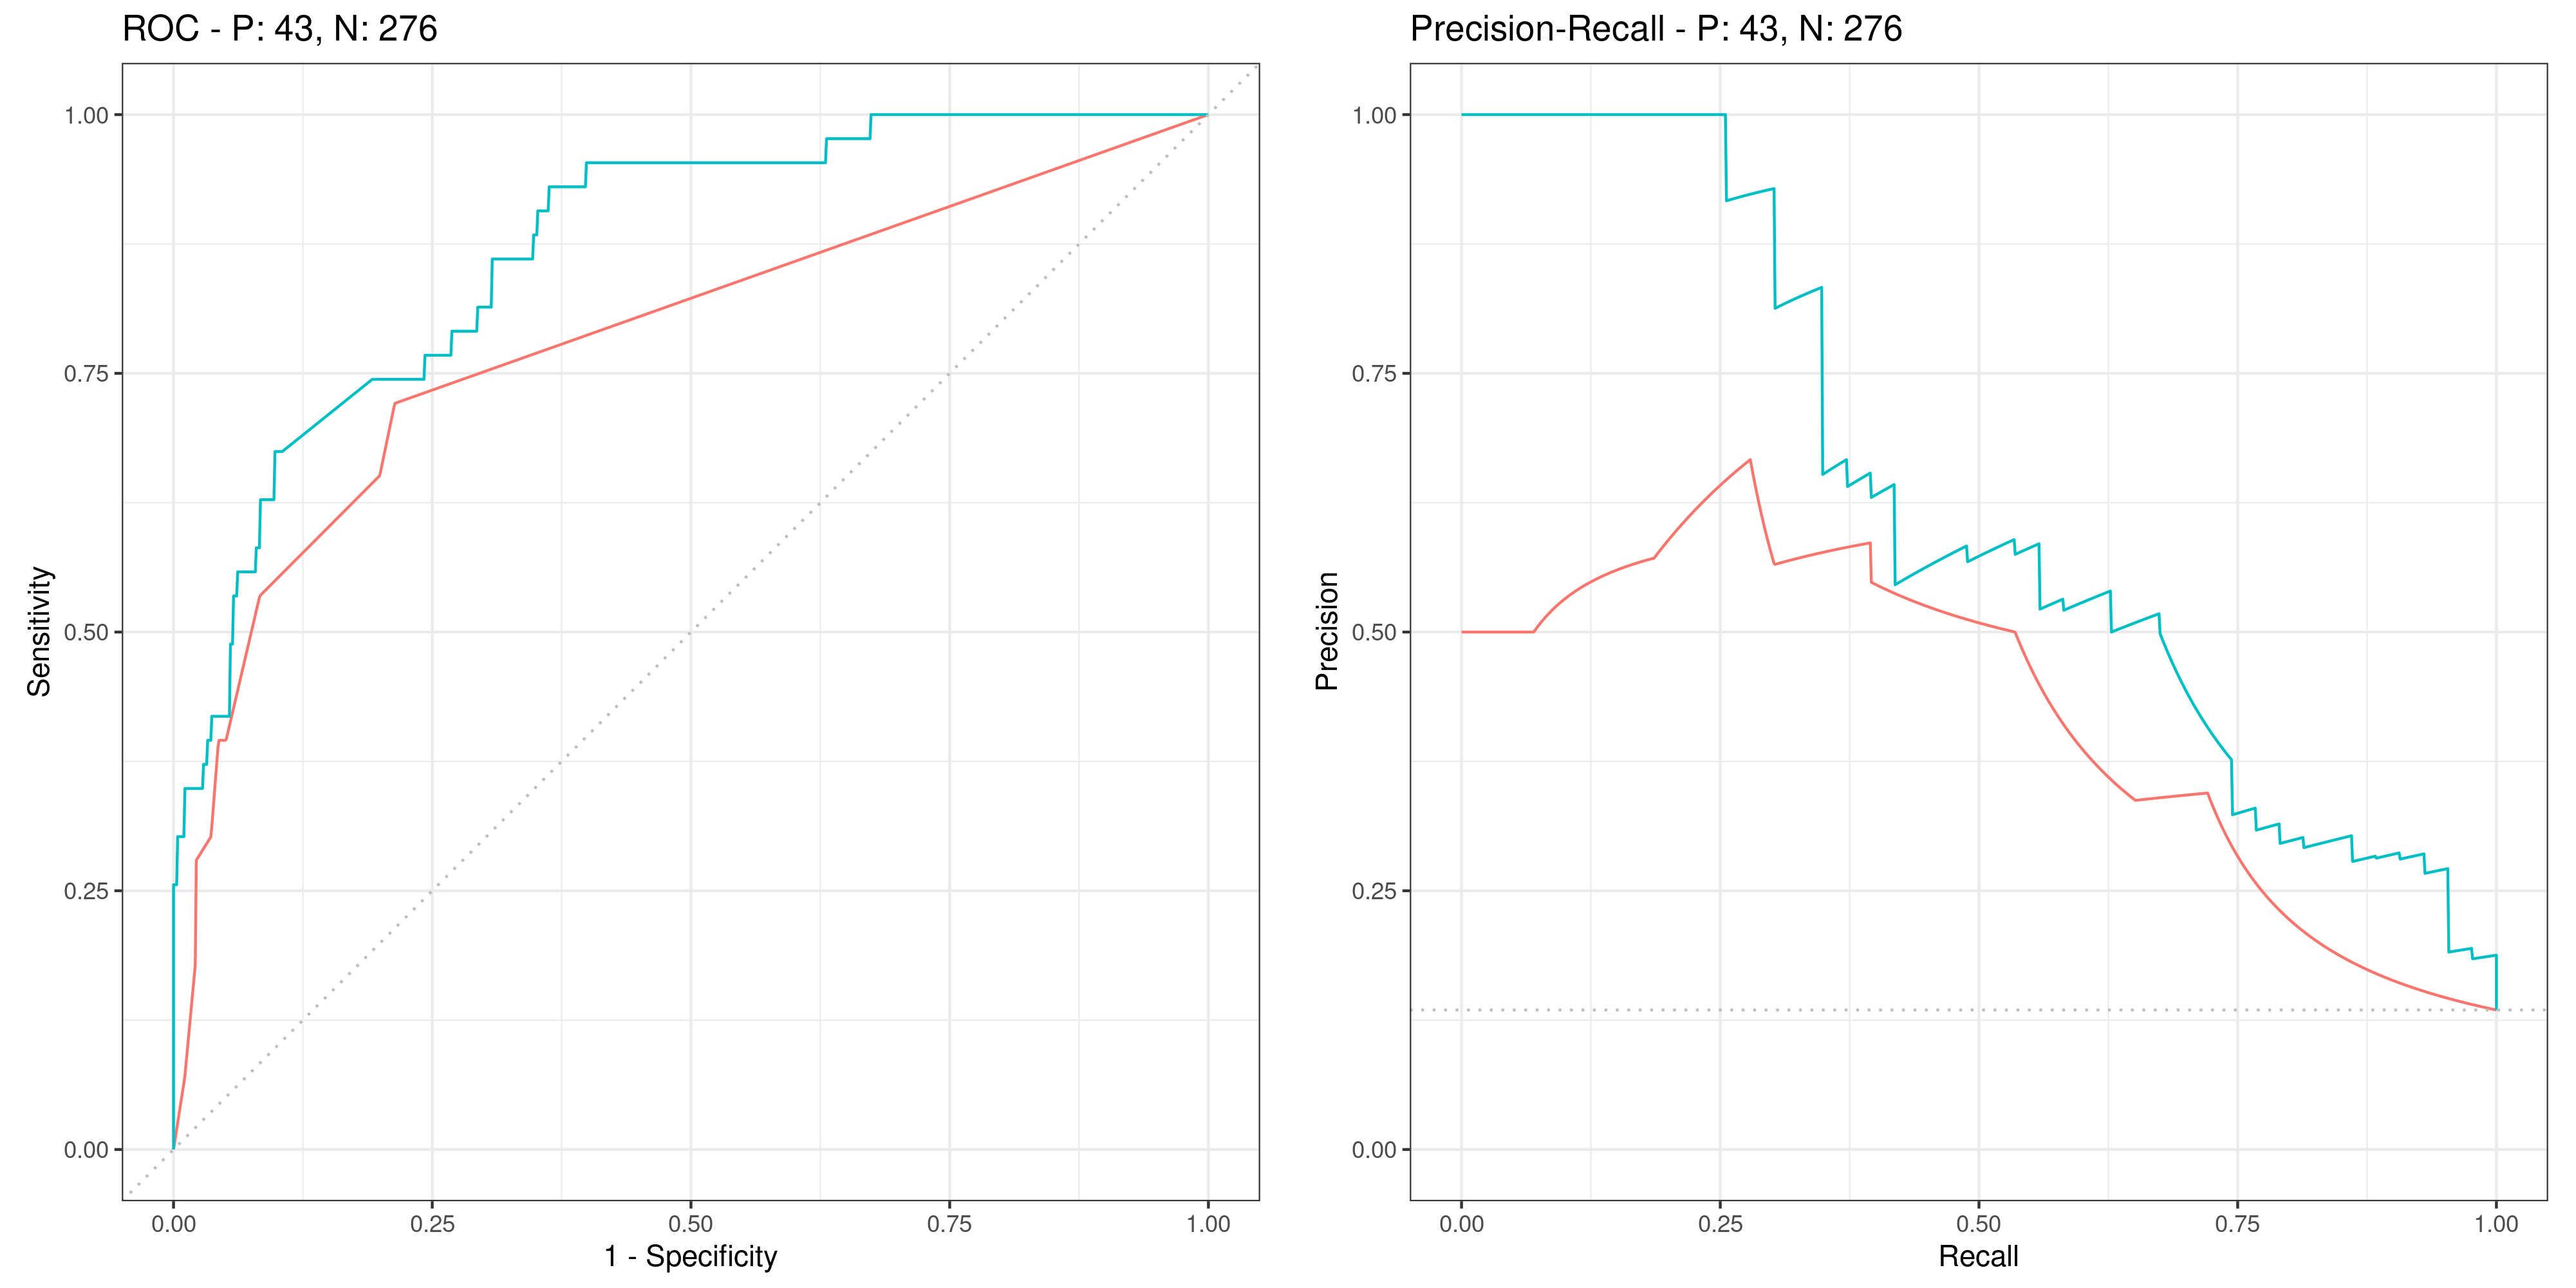
\includegraphics[width=\linewidth]{images/roc/no-outliers/z-score.png}
    }
    
    \quad
    
    \subfloat[Standardizzazione + PCA]{%
        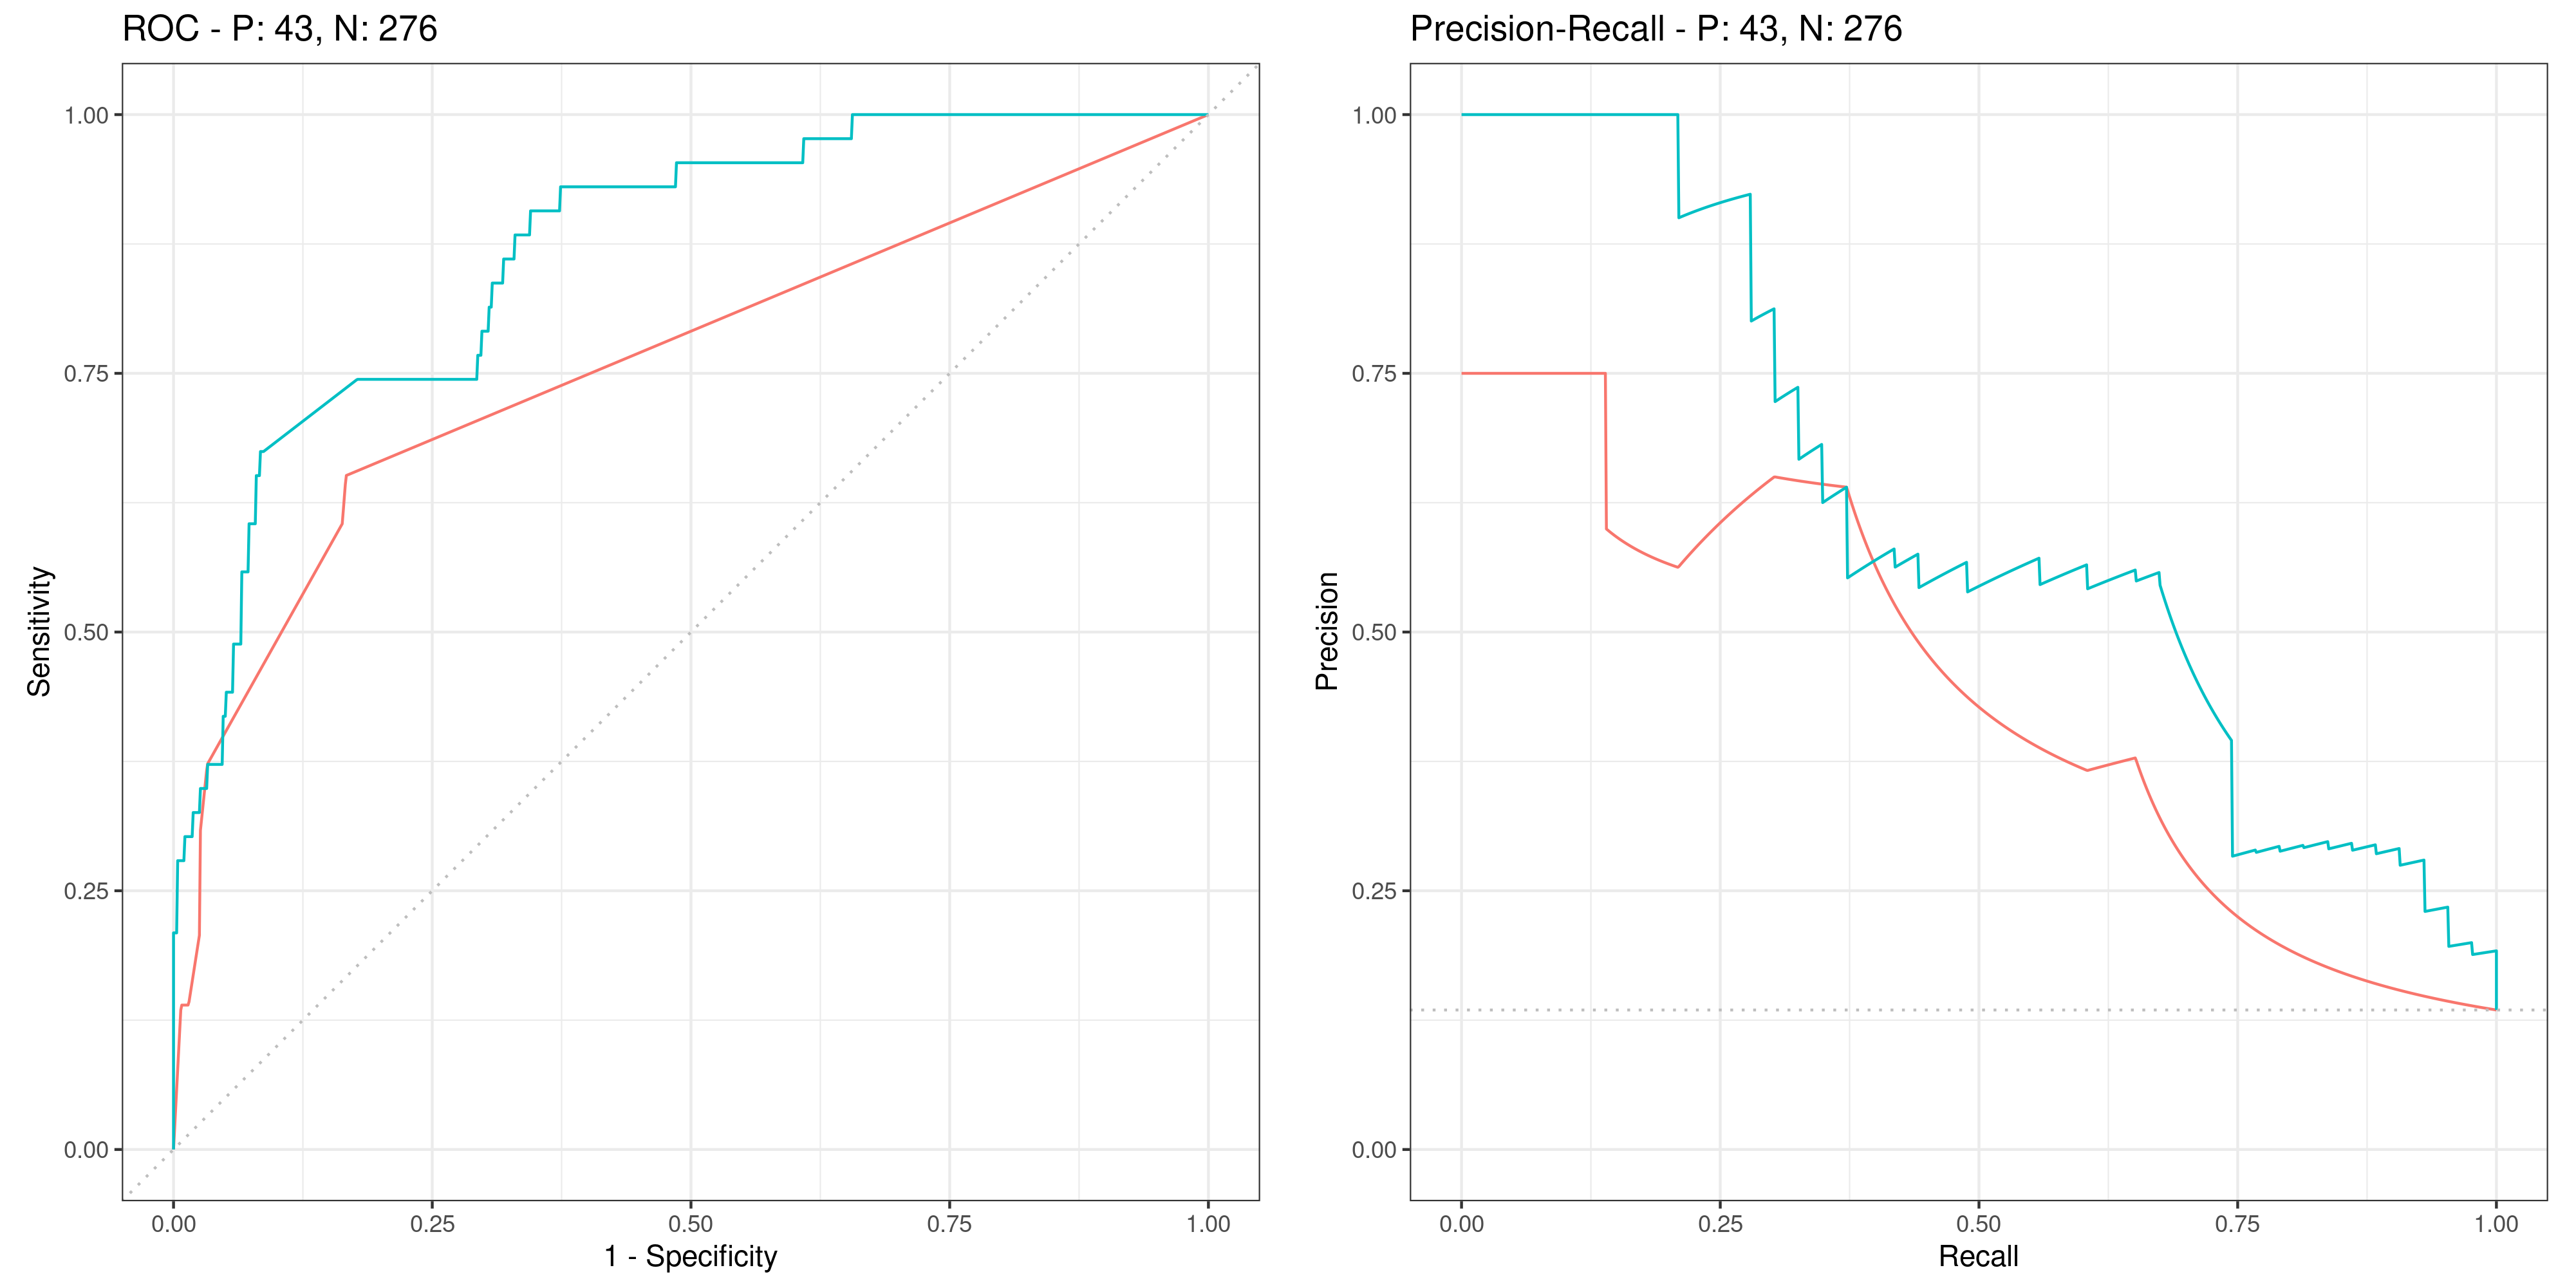
\includegraphics[width=\linewidth]{images/roc/no-outliers/pca.png}
    }

     \label{fig:roc_prc_svm}
    \caption{Curve ROC e PRC per i due modelli (cart: rosso, radiale: blu) sul testset senza outliers}
\end{figure}

\newpage

\noindent
Riassumiamo nuovamente i risultati presentati nelle tabelle sottostanti. Per scegliere i modelli migliori che verranno proposti in questo lavoro, è necessario analizzare le differenze tra Standardizzazione + PCA e Standardizzazione nel caso in cui gli outliers vengono mantenuti.
CART con Standardizzazione ha risultati migliori della controparte con Standardizzazione + PCA.
L'SVM radiale con Standardizzazione + PCA è leggermente migliore rispetto alla controparte con Standardizzazione.

\begin{table}[H]
\centering
\resizebox{\textwidth}{!}{%
\begin{tabular}{@{}ccccccccc@{}}
\toprule
\textbf{Models} & \textbf{Overall Accuracy} & \textbf{Precision} & \textbf{Recall} & \textbf{F1} & \textbf{ROC AUC} & \textbf{PRC AUC} & \textbf{95\% CI} & \textbf{P-Value} \\ \midrule
cart & 0.9154 & 0.83333 & \textbf{0.46512} & \textbf{0.59701} & 0.8476154 & 0.6564769 & (0.8792, 0.9435) & 0.003747 \\
svm & \textbf{0.9122} & \textbf{0.94118} & 0.37209 & 0.53333 & \textbf{0.9313279} & \textbf{0.7520759} & (0.8756, 0.9409) & 0.006404 \\ \bottomrule
\end{tabular}%
}
\caption{Risultati modelli scelti con Standardizzazione}
\label{tab:my-table}
\end{table}

\begin{table}[H]
\centering
\resizebox{\textwidth}{!}{%
\begin{tabular}{@{}ccccccccc@{}}
\toprule
\textbf{Models} & \textbf{Overall Accuracy} & \textbf{Precision} & \textbf{Recall} & \textbf{F1} & \textbf{ROC AUC} & \textbf{PRC AUC} & \textbf{95\% CI} & \textbf{P-Value} \\ \midrule
cart & 0.884 & 0.6 & \textbf{0.4186} & 0.49315 & 0.8194725 & 0.485855 & (0.8437, 0.917) & 0.18452 \\
svm & \textbf{0.9122} & \textbf{0.94118} & 0.37209 & \textbf{0.53333} & \textbf{0.9469161} & \textbf{0.7732596} & (0.8756, 0.9409) & 0.006404 \\ \bottomrule
\end{tabular}%
}
\caption{Risultati modelli scelti con Standardizzazione + PCA}
\label{tab:my-table}
\end{table}

\begin{table}[H]
\centering
\resizebox{\textwidth}{!}{%
\begin{tabular}{@{}ccccccccc@{}}
\toprule
\textbf{Models} & \textbf{Overall Accuracy} & \textbf{Precision} & \textbf{Recall} & \textbf{F1} & \textbf{ROC AUC} & \textbf{PRC AUC} & \textbf{95\% CI} & \textbf{P-Value} \\ \midrule
cart & 0.8746 & 0.56522 & \textbf{0.30233} & 0.39394 & 0.7817661 & 0.4226265 & (0.8332, 0.9089) & 0.347156 \\
svm & \textbf{0.8997} & \textbf{0.92308} & 0.27907 & \textbf{0.42857} & \textbf{0.8711662} & \textbf{0.6230968} & (0.8613, 0.9304) & 0.03864 \\ \bottomrule
\end{tabular}%
}
\caption{Risultati modelli scelti con Standardizzazione e rimozione outliers}
\label{tab:my-table}
\end{table}

\begin{table}[H]
\centering
\resizebox{\textwidth}{!}{%
\begin{tabular}{@{}ccccccccc@{}}
\toprule
\textbf{Models} & \textbf{Overall Accuracy} & \textbf{Precision} & \textbf{Recall} & \textbf{F1} & \textbf{ROC AUC} & \textbf{PRC AUC} & \textbf{95\% CI} & \textbf{P-Value} \\ \midrule
cart & 0.8746 & 0.58824 & \textbf{0.23256} & 0.33333 & 0.7598163 & 0.440484 & (0.8332, 0.9089) & 0.3472 \\
svm & \textbf{0.8934} & \textbf{0.90909} & \textbf{0.23256} & \textbf{0.37037} & \textbf{0.8684277} & \textbf{0.6079154} & (0.8543, 0.9251) & 0.07852 \\ \bottomrule
\end{tabular}%
}
\caption{Risultati modelli scelti con Standardizzazione + PCA e rimozione outliers}
\label{tab:my-table}
\end{table}

\noindent
Concludiamo che i modelli migliori sono CART con Standardizzazione e SVM radiale con Standardizzazione + PCA, entrambi mantenendo gli outliers.

\newpage

\section{Confronto fra i modelli scelti}
In questa sezione andiamo a confrontare i due modelli proposti per la trattazione del nostro problema.

\noindent
Mostriamo ora le matrici di confusione dei modelli testati sul testset composto da 319 istanze di cui 276 positive e 43 negative.
Dalle matrici di confusione possiamo vedere che i modelli non sembrano così diversi e come entrambi soffrono dello sbilanciamento del dataset. Infatti i nostri modelli classificano correttamente quasi tutte le istanze appartenenti alla classe maggioritaria, mentre sbagliano molto di più sulla classe minoritaria.

\begin{figure}[H]
    \centering
    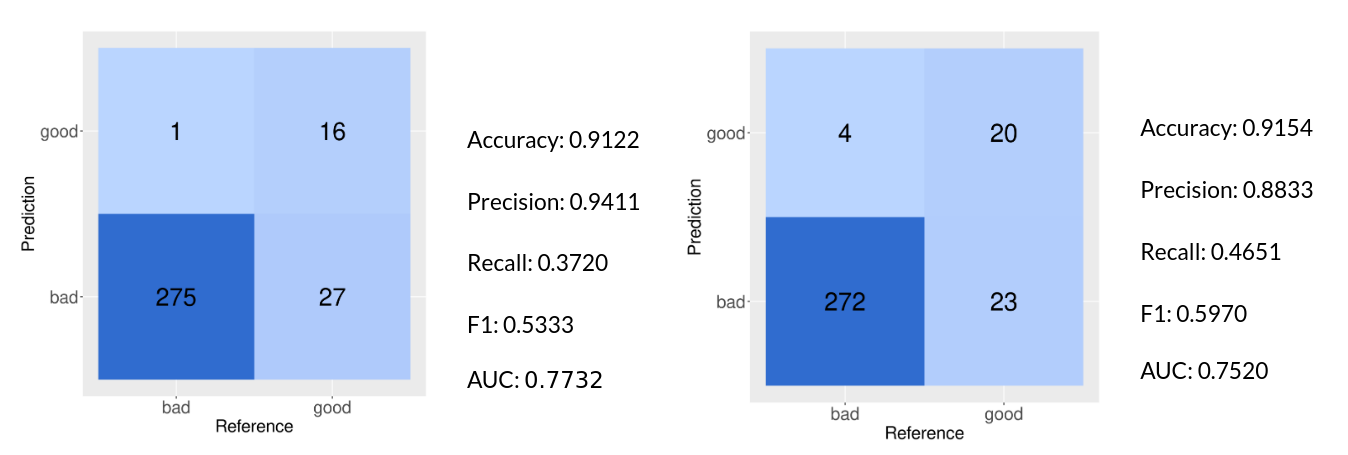
\includegraphics[width=\linewidth]{images/comparison/comparison2.png}
     \label{fig:confusion_matrix}
    \caption{Matrice di confusione sul testset per SVM Radiale con Standardizzazione + PCA (sinistra) e CART con Standardizzazione (destra)}
\end{figure}

\noindent
Comparando le metriche ottenute dai due modelli possiamo vedere come non ci sia una grossa differenza, tra alti valori di Precision e bassi valori di Recall, non considerando l'Accuracy come già detto precedente non è un buon indicatore. L'AUC è un indicatore migliore infatti notiamo che l'SVM radiale supera CART in AUC e Precision, mentre CART è migliore in Recall e F1.

\newpage

\noindent
Mostrando la ROC e la PRC è possibile vedere come l'SVM radiale superi CART in entrambe seppure di poco, rispettivamente 0.9469161/0.7732596 0.9313279/0.7520759.
\begin{figure}[H]
    \centering
    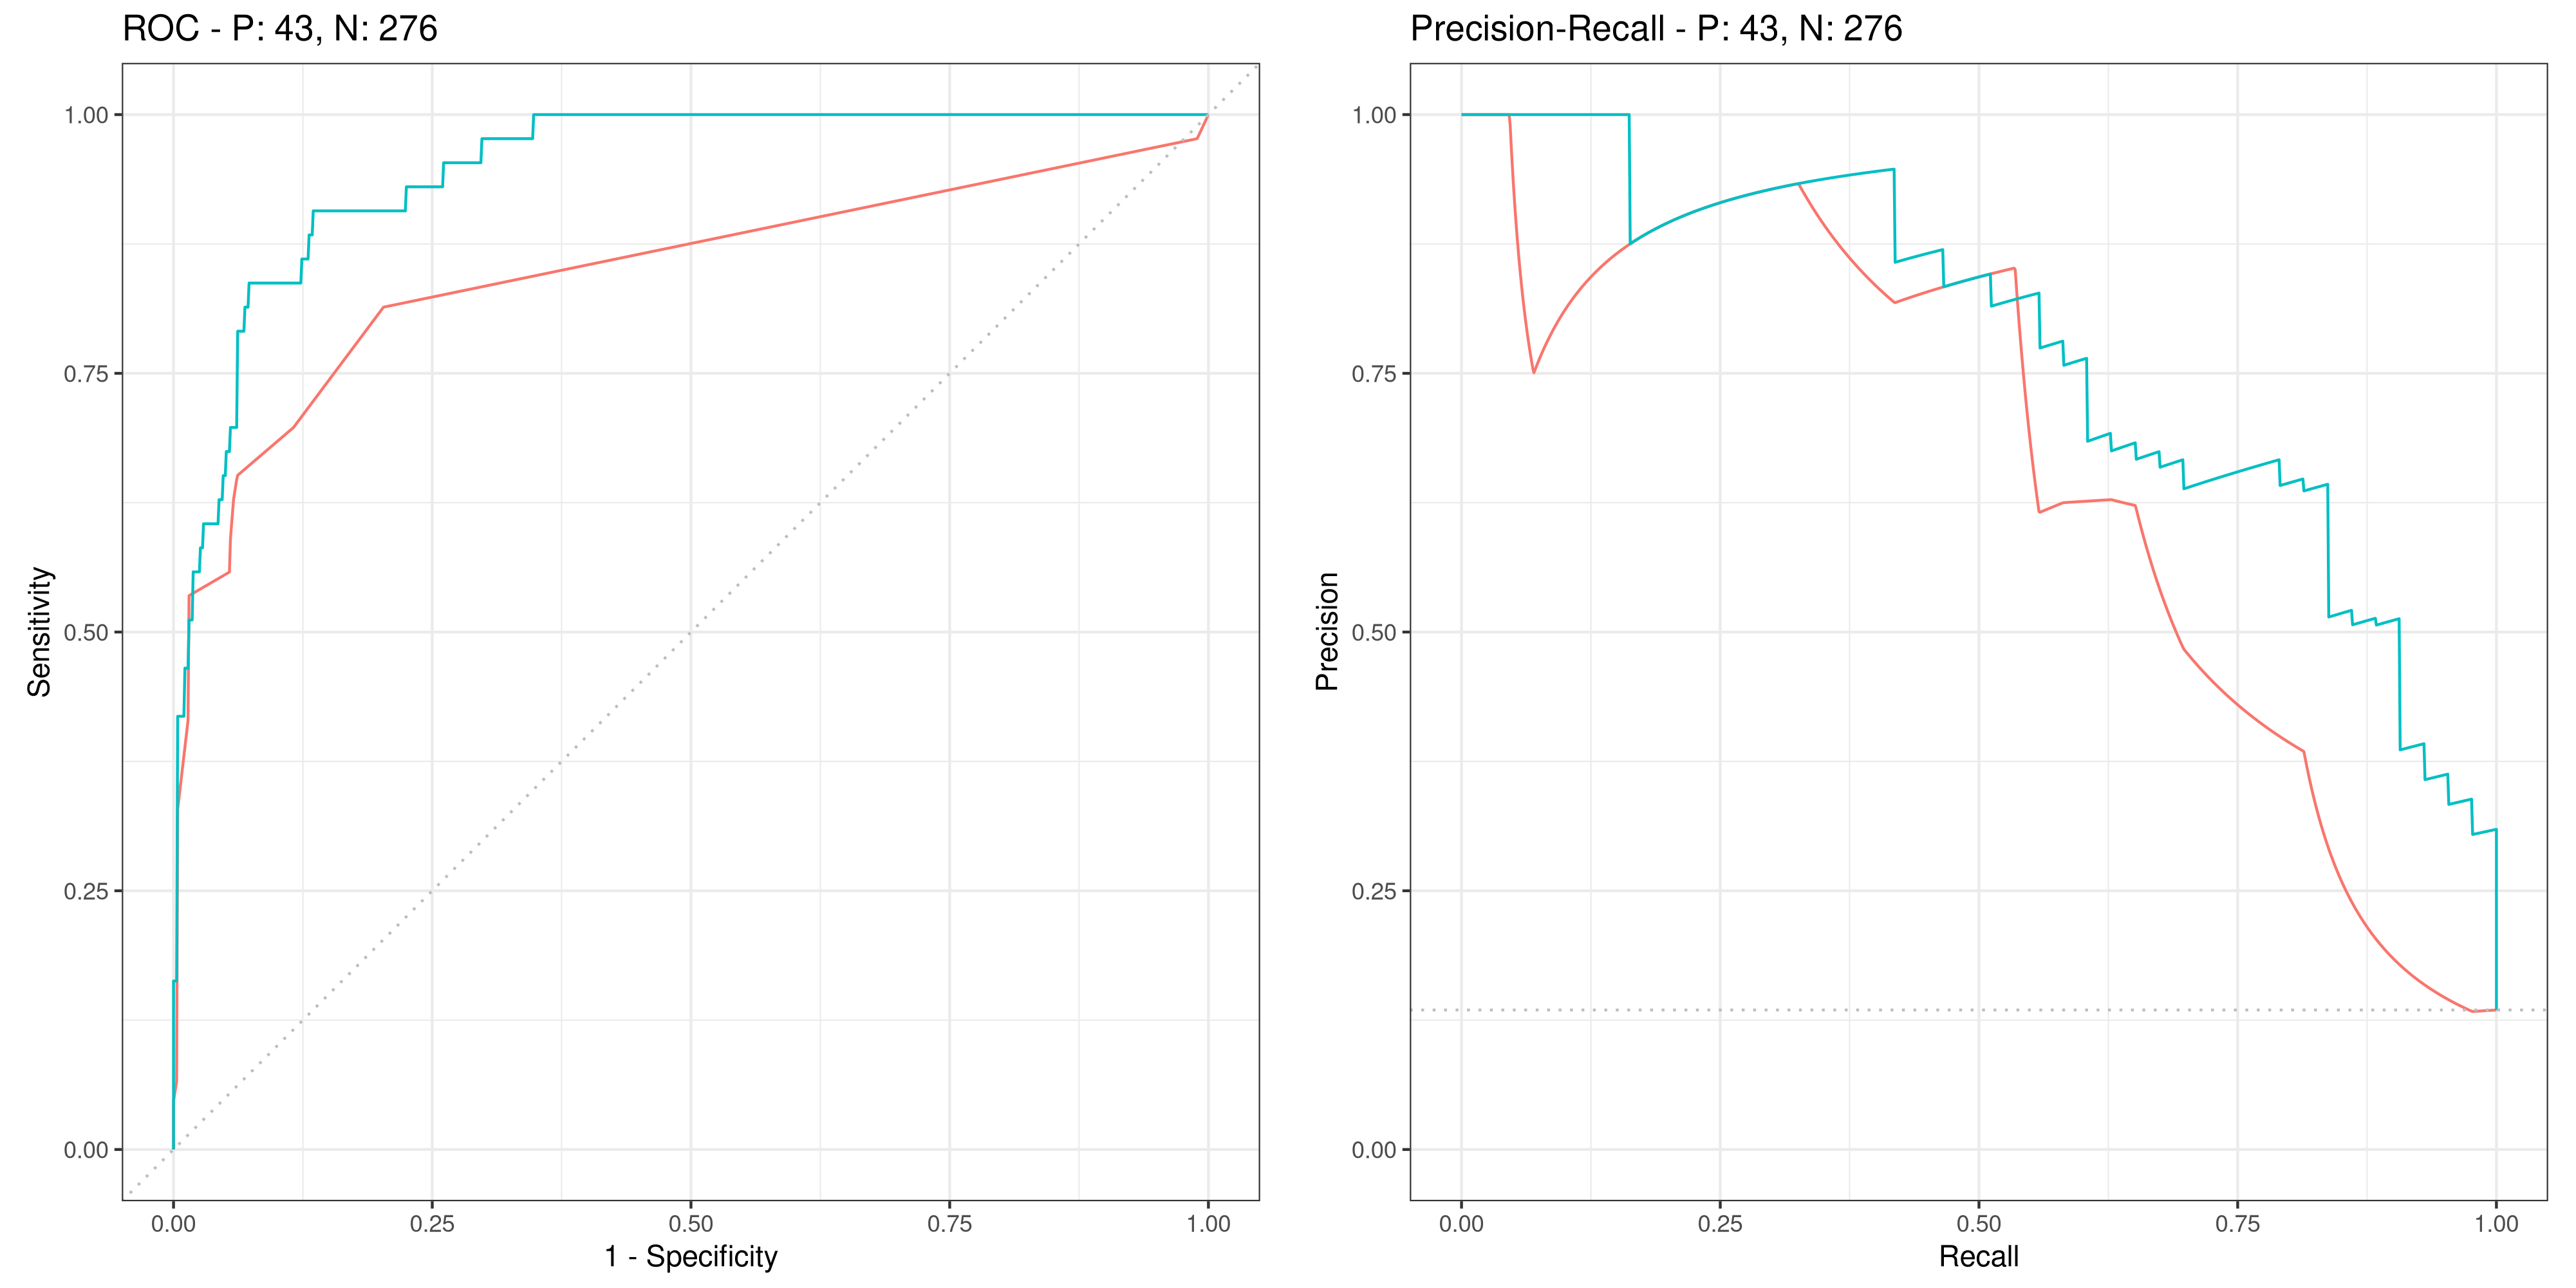
\includegraphics[width=\linewidth]{images/comparison/best/best_roc.png}
     \label{fig:roc_prc_modelli_proposti}
    \caption{Grafici ROC e PRC per i due modelli proposti, (cart: rosso, radiale: blu)}
\end{figure}

\begin{figure}[H]
    \centering
    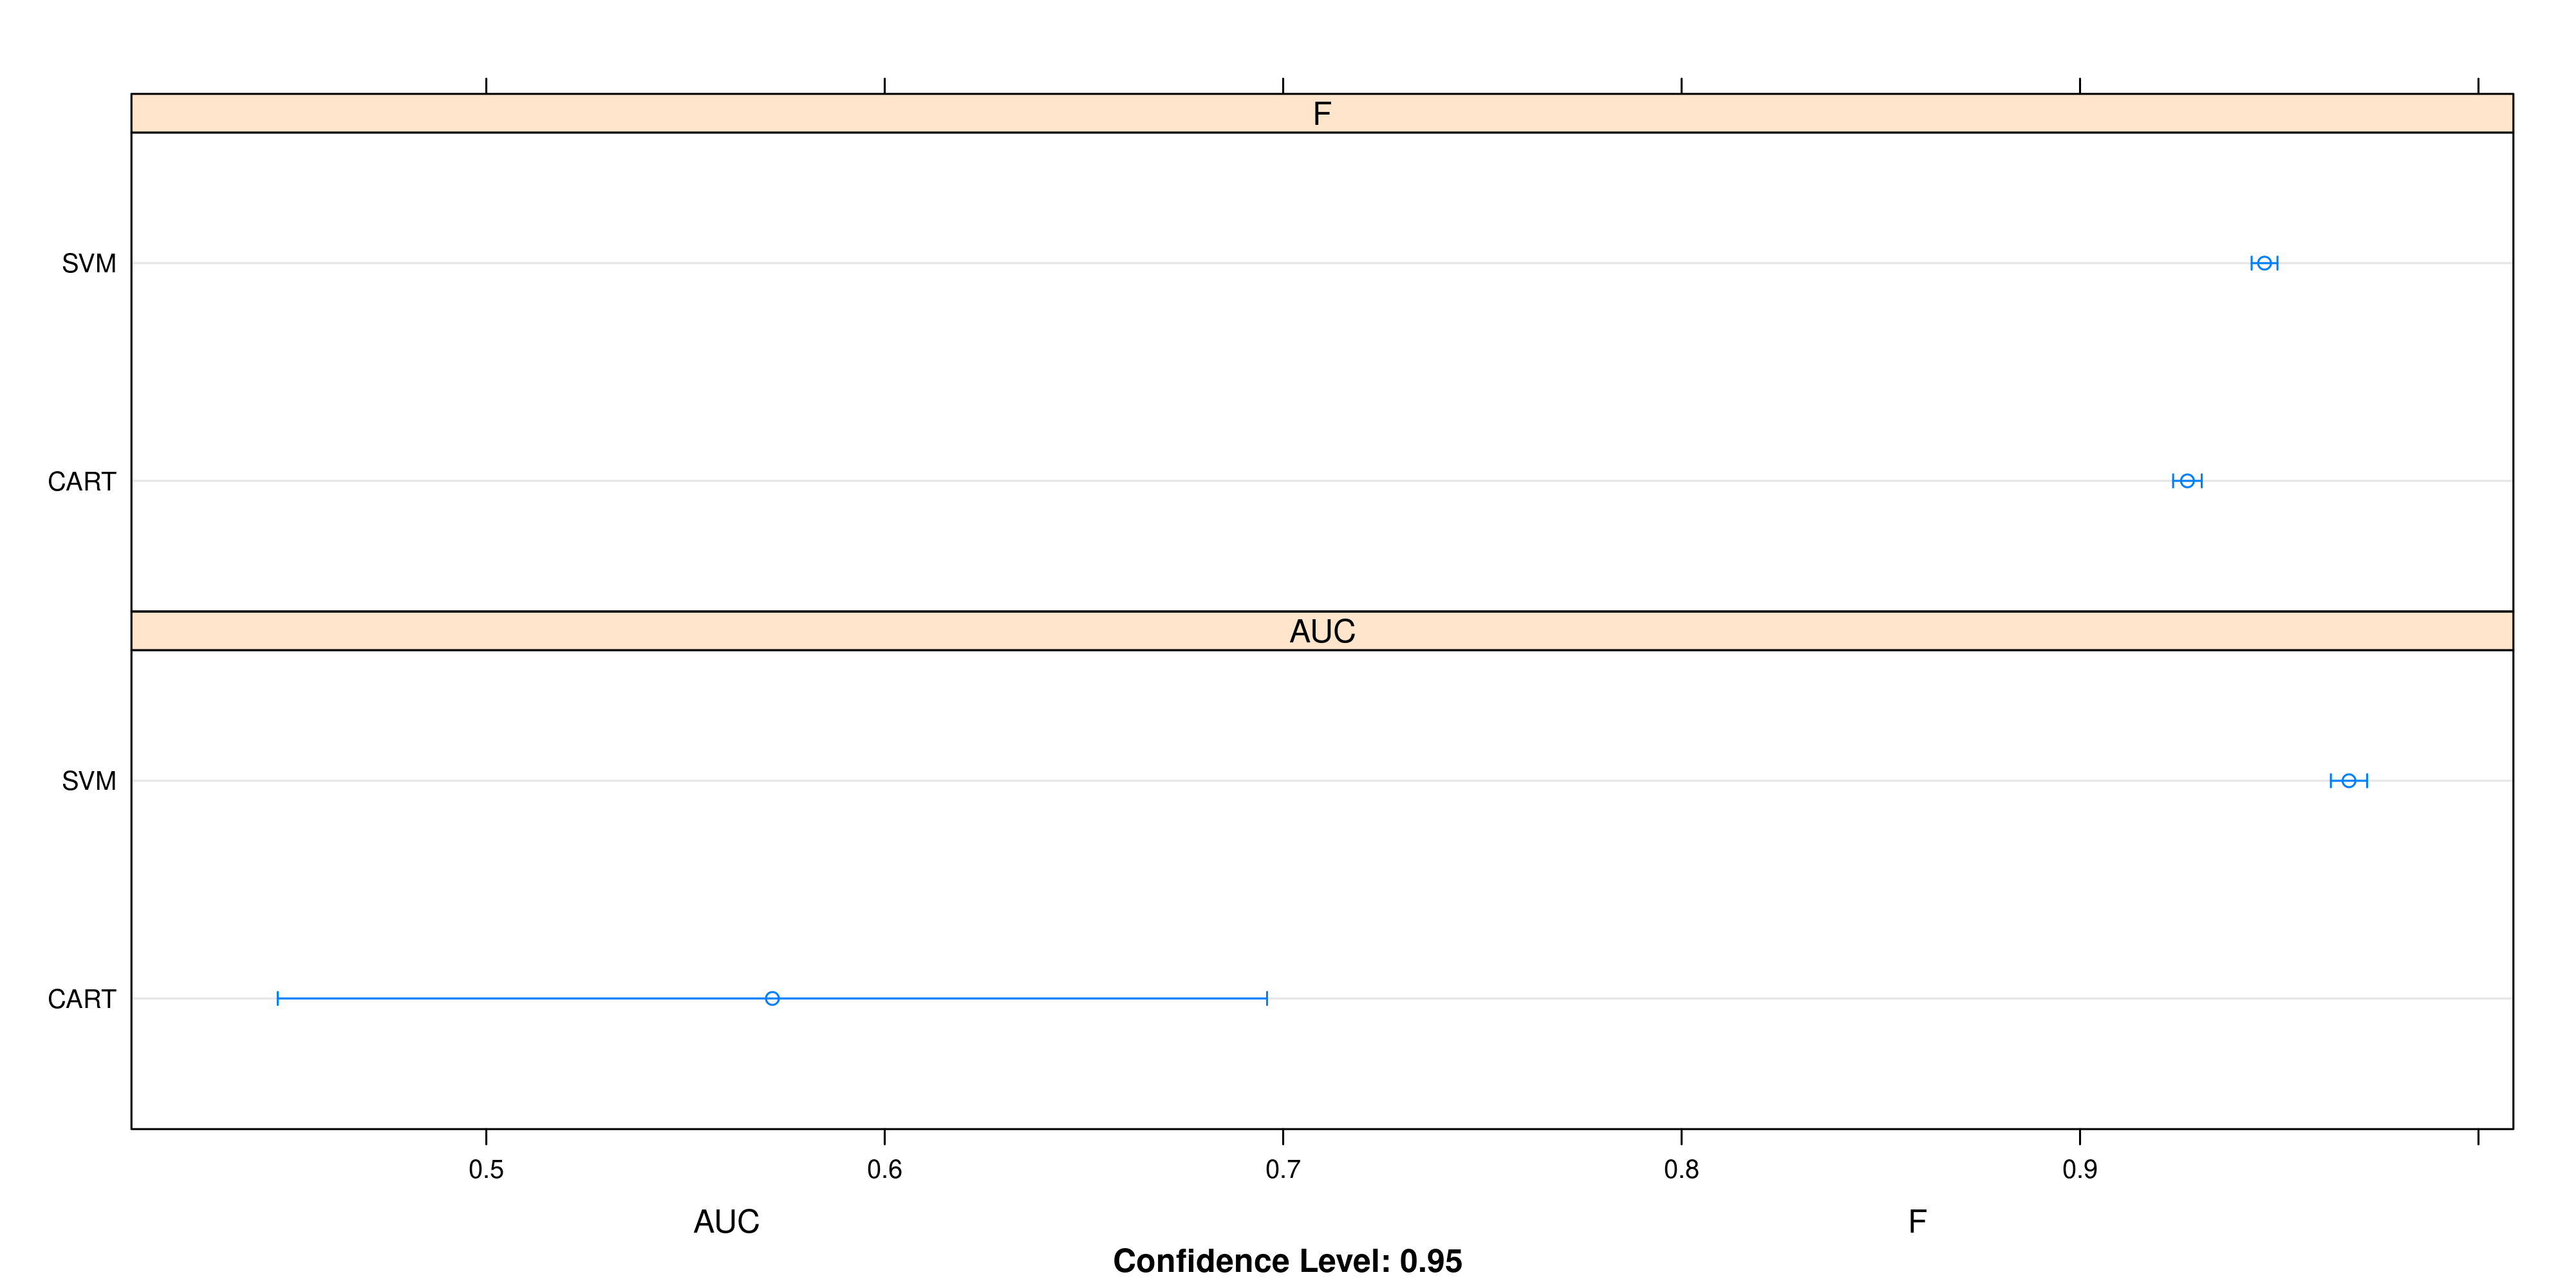
\includegraphics[width=\linewidth]{images/comparison/best/best_dotplot_af.png}
     \label{fig:ci1_modelli_proposti}
    \caption{Intervalli di confidenza dei modelli proposti per AUC e F1, (svmRadial: svm radiale, rpart2: cart)}
\end{figure}

\begin{figure}[H]
    \centering
    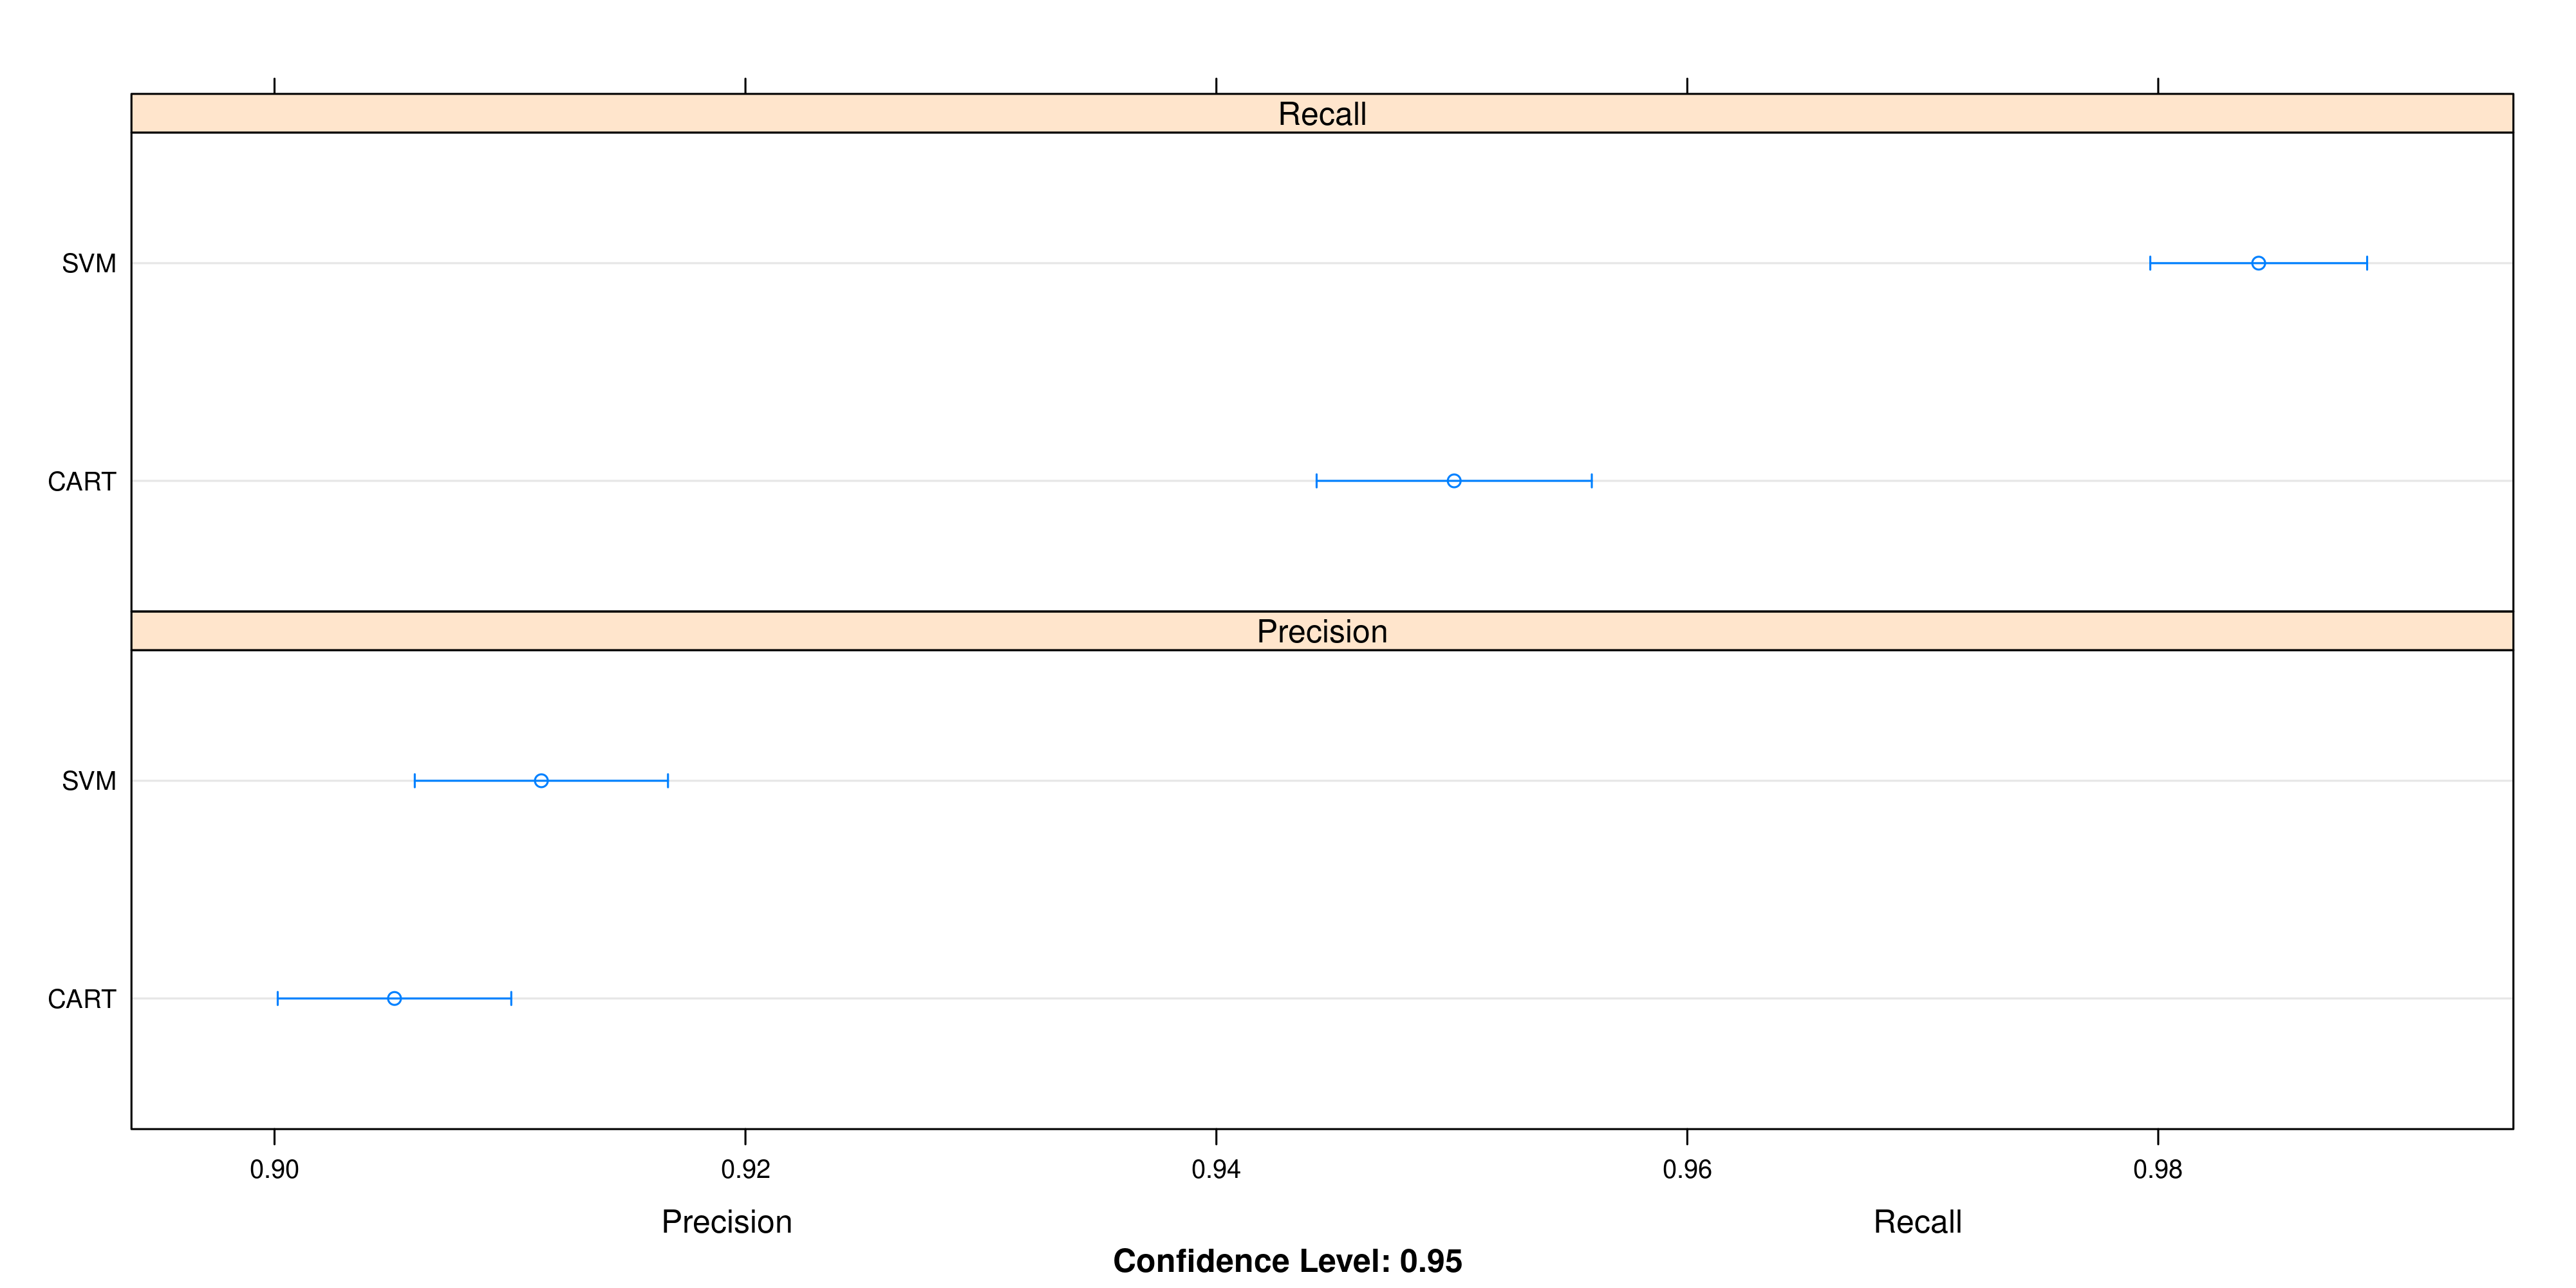
\includegraphics[width=\linewidth]{images/comparison/best/best_dotplot_pr.png}
     \label{fig:c21_modelli_proposti}
    \caption{Intervalli di confidenza dei modelli proposti per Precision e Recall, (svmRadial: svm radiale, rpart2: cart)}
\end{figure}

\noindent
Dagli intervalli di confidenza al 95\% sono visibili leggere differenze in Precision e F1, si può notare una differenza maggiore nella Recall. CART ha un CI molto grande rispetto all'AUC.

\vspace{5mm}
\noindent
Infine osservando i tempi di addestramento vediamo come CART prevede un tempo molto basso di 8.649s, al contrario l'SVM radiale prevede un costo più oneroso di 1827.793s. Dovendo scegliere un modello tra i due proposti l'SVM risulta migliore, nonostante abbia performance simili a CART ed un costo più elevato, poiché CART ha un intervallo di confidenza al 95\% troppo grande rispetto all'AUC.


\chapter{Risultati}
\label{ch:risultati}

\chapter{Conclusioni}
\label{ch:conclusioni}
In questa trattazione si è visto un problema di classificazione per la qualità del vino. Si è visto che con 10 classi il problema era difficile per la mancanza di dati per alcune classi. Si è passato quindi ad un problema binario con vini di buona qualità e vini di cattiva qualità, inoltre si è preferito analizzare solo una tipologia di vino, limitandosi al vino rosso.

\noindent
Durante la fase di analisi dei dati si è visto come i dati siano sbilanciati ed alcuni attributi presentassero distribuzioni fortemente asimmetriche.

\noindent
Sono stati identificati gli outliers e si è notato che la loro numerosità costituisce solamente il 2.88\% del training set. E' stato deciso inizialmente di non rimuoverli ed aspettare la fase di esperimenti per prendere una decisione in seguito ai risultati ottenuti.

\noindent
Analizzando le correlazioni abbiamo notato bassi valori tra i vari attributi e la qualità, il che comporta una difficoltà nel distinguere le due classi.
Inoltre con la rimozione degli outliers aumentano leggermente i valori di correlazione, anche se rimangono abbastanza medio bassi.


\noindent
E' stata effettuata una PCA e come previsto dai valori bassi di correlazione non ci sono stati grandi miglioramenti. Con il 95\% di varianza spiegata vengono tenuti 9 degli 11 attributi.

\newpage

\noindent
I modelli che sono stati scelti per questa trattazione sono CART e SVM, per quest'ultimo sono stati analizzati diversi kernel. Questi modelli di solito sono abbastanza robusti agli outliers e sono addestrabili anche con relativamente pochi dati.
Dato che l'SVM richiede che venga effettuato un pre processing sui dati, è stato eseguito una standardizzazione con z-score.

\noindent
Addestrare questi modelli ha previsto alcune accortezze a causa dello sbilanciamento dei dati. E' stata usata una 5-fold cross validation stratificata con 5 ripetizioni per ottenere risultati più attendibili. La metrica usata per la scelta del modello migliore è l'AUC della PRC.

\noindent
Dagli esperimenti è risultato che il kernel migliore per SVM è quello radiale. Questo modello è stato confrontato con CART al variare del pre processing.
I due modelli migliori identificati sono SVM radiale con Standardizzazione + PCA e CART con Standardizzazione, entrambi mantenendo gli outliers.

\noindent
I modelli proposti presentano performance molto simili con alti valori di Precision e bassi di Recall. Le uniche differenze sono nei costi di addestramento e gli intervalli di confidenza sull'AUC della PRC, motivo per il quale, tra i due, il migliore risulta essere l'SVM.

\noindent
I risultati ottenuti non sono ottimi, comunque comprensibili, poichè i dati sono sbilanciati e le feature poco discriminanti.
Possibili sviluppi futuri, oltre la raccolta di nuovi dati, possono essere gestire lo sbilanciamento con tecniche di undersampling o oversampling esempio SMOTE \cite{chawla2002smote}, altri modelli più sofisticati possono essere utilizzati come le Random Forest \cite{biau2016random}.
Inoltre si potrebbe estendere il problema a più classi o considerare anche il vino bianco.


% INCLUSIONE APPENDICE
% \appendix
% \include{chapters/app_a}

% BIBLIOGRAFIA
\phantomsection
\addcontentsline{toc}{chapter}{\refname}\nocite{*}
\printbibliography

\end{document}
